\documentclass[]{article}

\usepackage{pgfplots} 
\usepackage{graphicx}
\usepackage{subfigure}
\usepackage{floatflt}
\usepackage{float}
\usepackage{hyperref}
\usepackage{mathtools}
\usepackage{tikz}
\usepackage{pgf}
\usepackage{cleveref}
\usepackage{xcolor}
\usetikzlibrary{calc,patterns,angles,quotes}
\usepackage{makecell}
\usepackage{tabularx}
\usepackage{listings}
\usepackage{svg}
\usepackage{tablefootnote}
\usepackage[most]{tcolorbox}

\newcommand{\inctrimpic}[2][1]
{\includegraphics[trim=0 200 0 200, clip, width=#1\linewidth]{#2}}

\include{LaTeX.Listings}
\lstset{style=colorEX}

%opening
\title{Semi-Automatic Portable Star Tracker}
\author{Simone Fabbri \\ simone.fabbri8@studio.unibo.it}

\begin{document}

\maketitle

\begin{figure}[h]
	\centering
	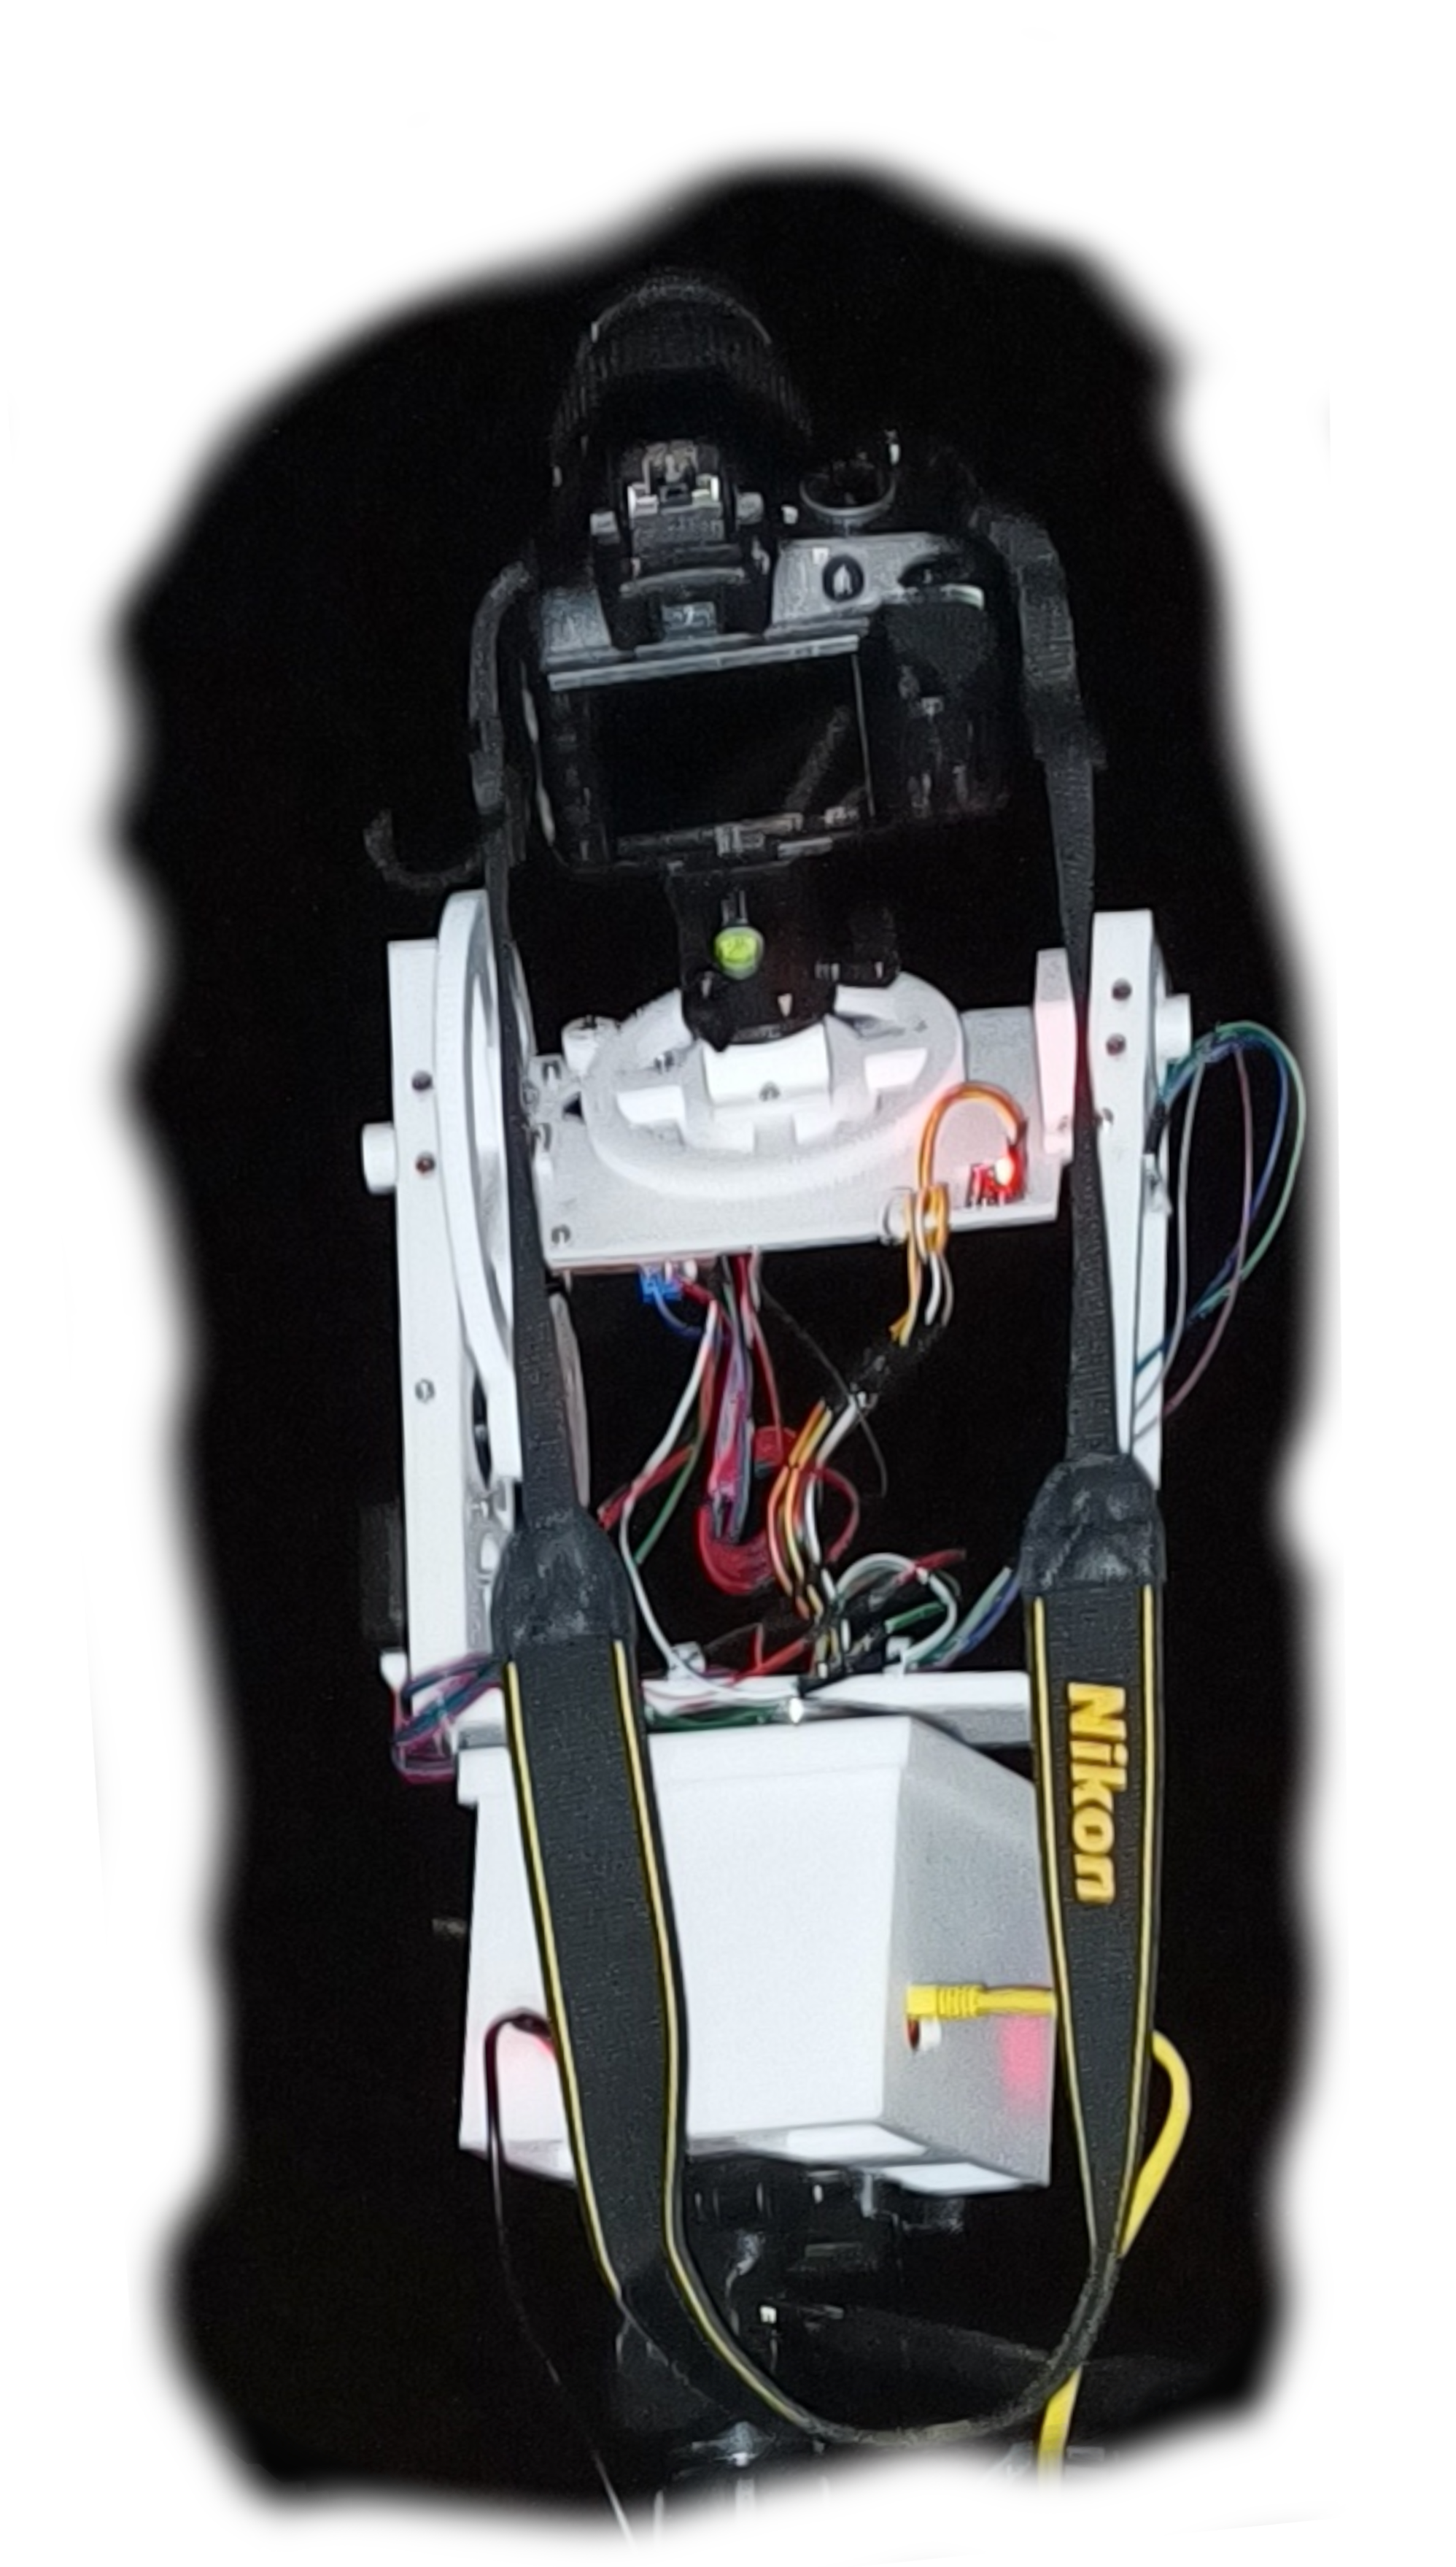
\includegraphics[width=0.5\linewidth, height=10cm]{images/cover/cover}
\end{figure}

\begin{abstract}
This is the report of the project developed for the making class at the Computer Science course, university of Bologna.
\\
The scope of this project is to make a portable star tracker, with auto-alignement capability. Star trackers are very useful to photograph stars at night, since longer exposures are required. 
\\
In the following sections will be discussed the main motivations behind this project, the technical details and the conclusion of the report.

\end{abstract}

\begin{tcolorbox}[colback=red!5!white,colframe=red!75!black]
	\textbf{Warning} this is \textit{experimental} work. While the procedure is accurately documented and replicable, the end result is not working, i.e. it does not produce the expected results according to the design goals. The "Results" section shows what can be accomplished in terms of obtainable images. A list of errors and problems can be found in the "Conclusion" section. 
\end{tcolorbox}

\section{Introduction}

\begin{floatingfigure}[r]{0.30\linewidth}
	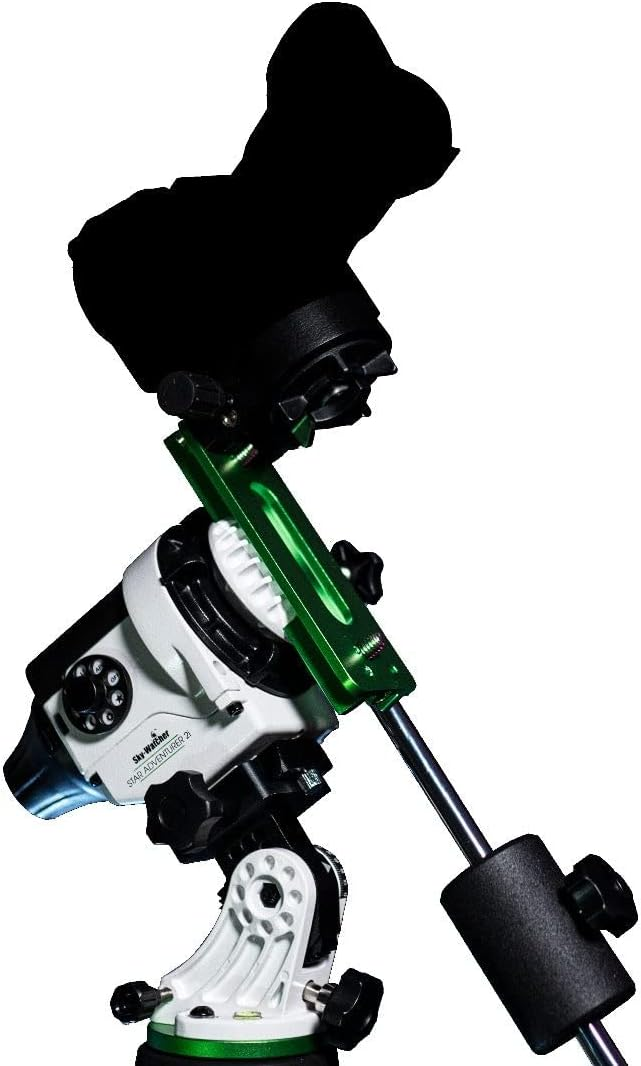
\includegraphics[width=0.27\linewidth]{images/introduction/startracker}
	\caption{A commercial 500\$ star tracker, the \textit{Skywatcher Star Adventurer 2i.\\}}
\end{floatingfigure}


Capture images of stars is not a trivial task: since they don't emit a lot of light, cameras have a harder time capturing it. 

The only way to capture in a somewhat recognizable way a scarce source of light, is to use a longer time exposure: keeping the camera sensor open for longer time, allows more light to pass. 

But this can only work well for still objects: while stars technically do not move, the earth does, thus the stars seem to move during the night. If a sensor is left open for too much time, a so called "star trail" will start to appear, because the stars will have moved since the start of the capture and their traces will be left on the camera sensor.

To contrast this effect, two solution were developed in the field of photography: 

\begin{itemize}
	\item photo stacking
	\item star tracking
\end{itemize}

The first solution, \textbf{photo stacking}, consists of taking multiple shorter pictures where the stars appear still, i.e. without trails and, using specialized software, "merge" them together. This allows to reduce the noise\footnote{There are different source of noise for a digital image, but the main one in this context is shot noise\cite{shotnoise}: objects emit photons in a random way, and although this is difficult to perceive for humans, it is more evidently in long exposure, dark scene photos, so much that becomes apparent in the photos. } 
in the image, and obtain better quality images.

The second solution is to simply move the camera according to the movement of the stars, using a tool called \textbf{star tracker}: in this way, we can keep the sensor for as long as we want, and the effect of the movement will not be in the image, except for objects in the foreground (e.g. trees, mountains, houses...).



The next sections present the desired features for an optimal solution, the existing solutions for star tracking, and the process of develop a new star tracking system.

\subsection{Requirements for the optimal system}

There are 3 main design goals:
\begin{enumerate}
	\item The star tracker can be used with any commercial DSLR camera and lens.
	\item The star tracker is portable.
	\item The star tracker can be used with any commercial tripod.
\end{enumerate}

These requirements offer the same capabilities of any major commercial solution, thus they define the best solution a \textit{maker} can hope to achieve (given that the total cost is less of a commercial solution) to replicate the same capabilities. In reality, due to limitation of experience, resources, available technologies... the first requirement is relaxed and substituted with the following one:
\begin{enumerate}
	\item The star tracker can be used with any \textbf{small} commercial DSLR camera, \textbf{where "small" means that camera body plus lens should be at maximum about 1 kg.}
\end{enumerate}

Furthermore we want to add another capability:


\begin{enumerate}
	\setcounter{enumi}{3}
	\item The star tracker can auto-align itself, with little to no need for the user to interact with it.
\end{enumerate}

The problem of alignment will be discussed later.


\subsection{Related work}
In this section the focus is on "DIY" or open source solutions, not on commercial ones.

To the best of my knowledge, there are two main projects for DIY star trackers, none of witch fully satisfies the requirement.

\subsubsection{The Micro Scope}

This is a fully functional star tracker \cite{microscope} (technically is a GOTO telescope, but has also tracking capabilities). It can be mounted on a tripod, so it is very portable. The problem is that it not a DSLR star tracker, but there is an embedded camera, so the user cannot attach it's own camera. 

\begin{figure}[H]
	\centering
	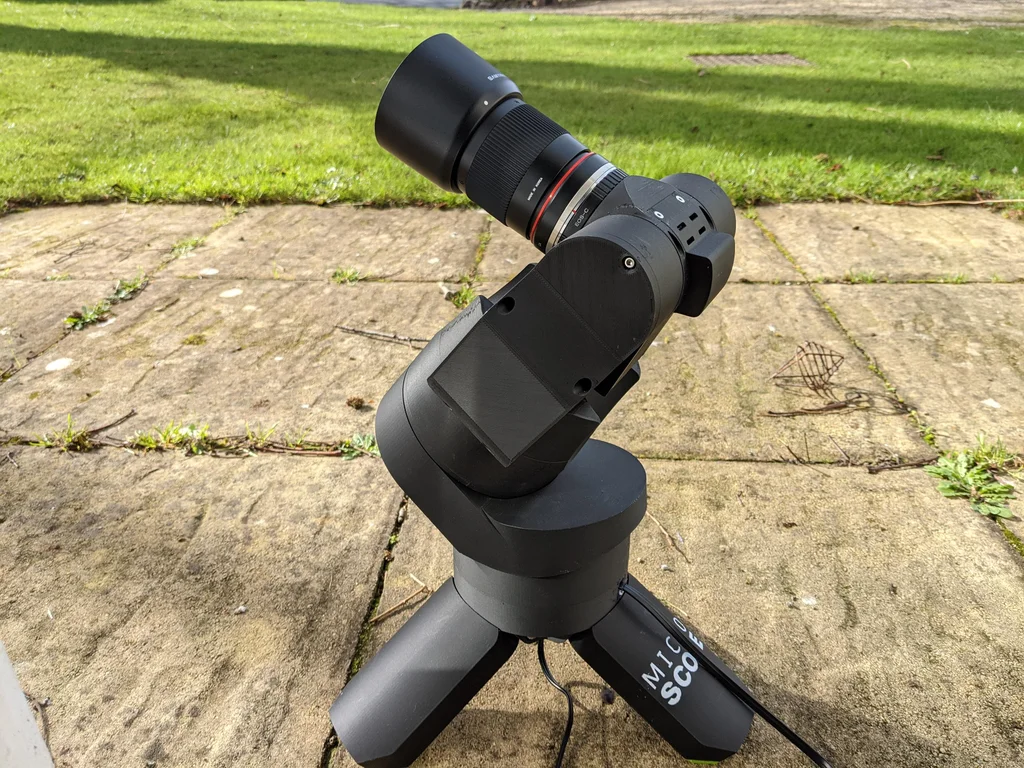
\includegraphics[width=0.7\linewidth]{images/background/themicroscope}
	\caption{The Micro Scope DIY goto telescope and tracker.}
\end{figure}

\subsubsection{OpenAstroTracker}

This design was proposed by the reddit user Intercipere \cite{openastrotracker}. This is a very compelling project and probably the best DIY star tracker (and it also has GOTO capabilities), but it has its own standing platform and is considerably bigger than commercial solutions. 

\begin{figure}[H]
	\centering
	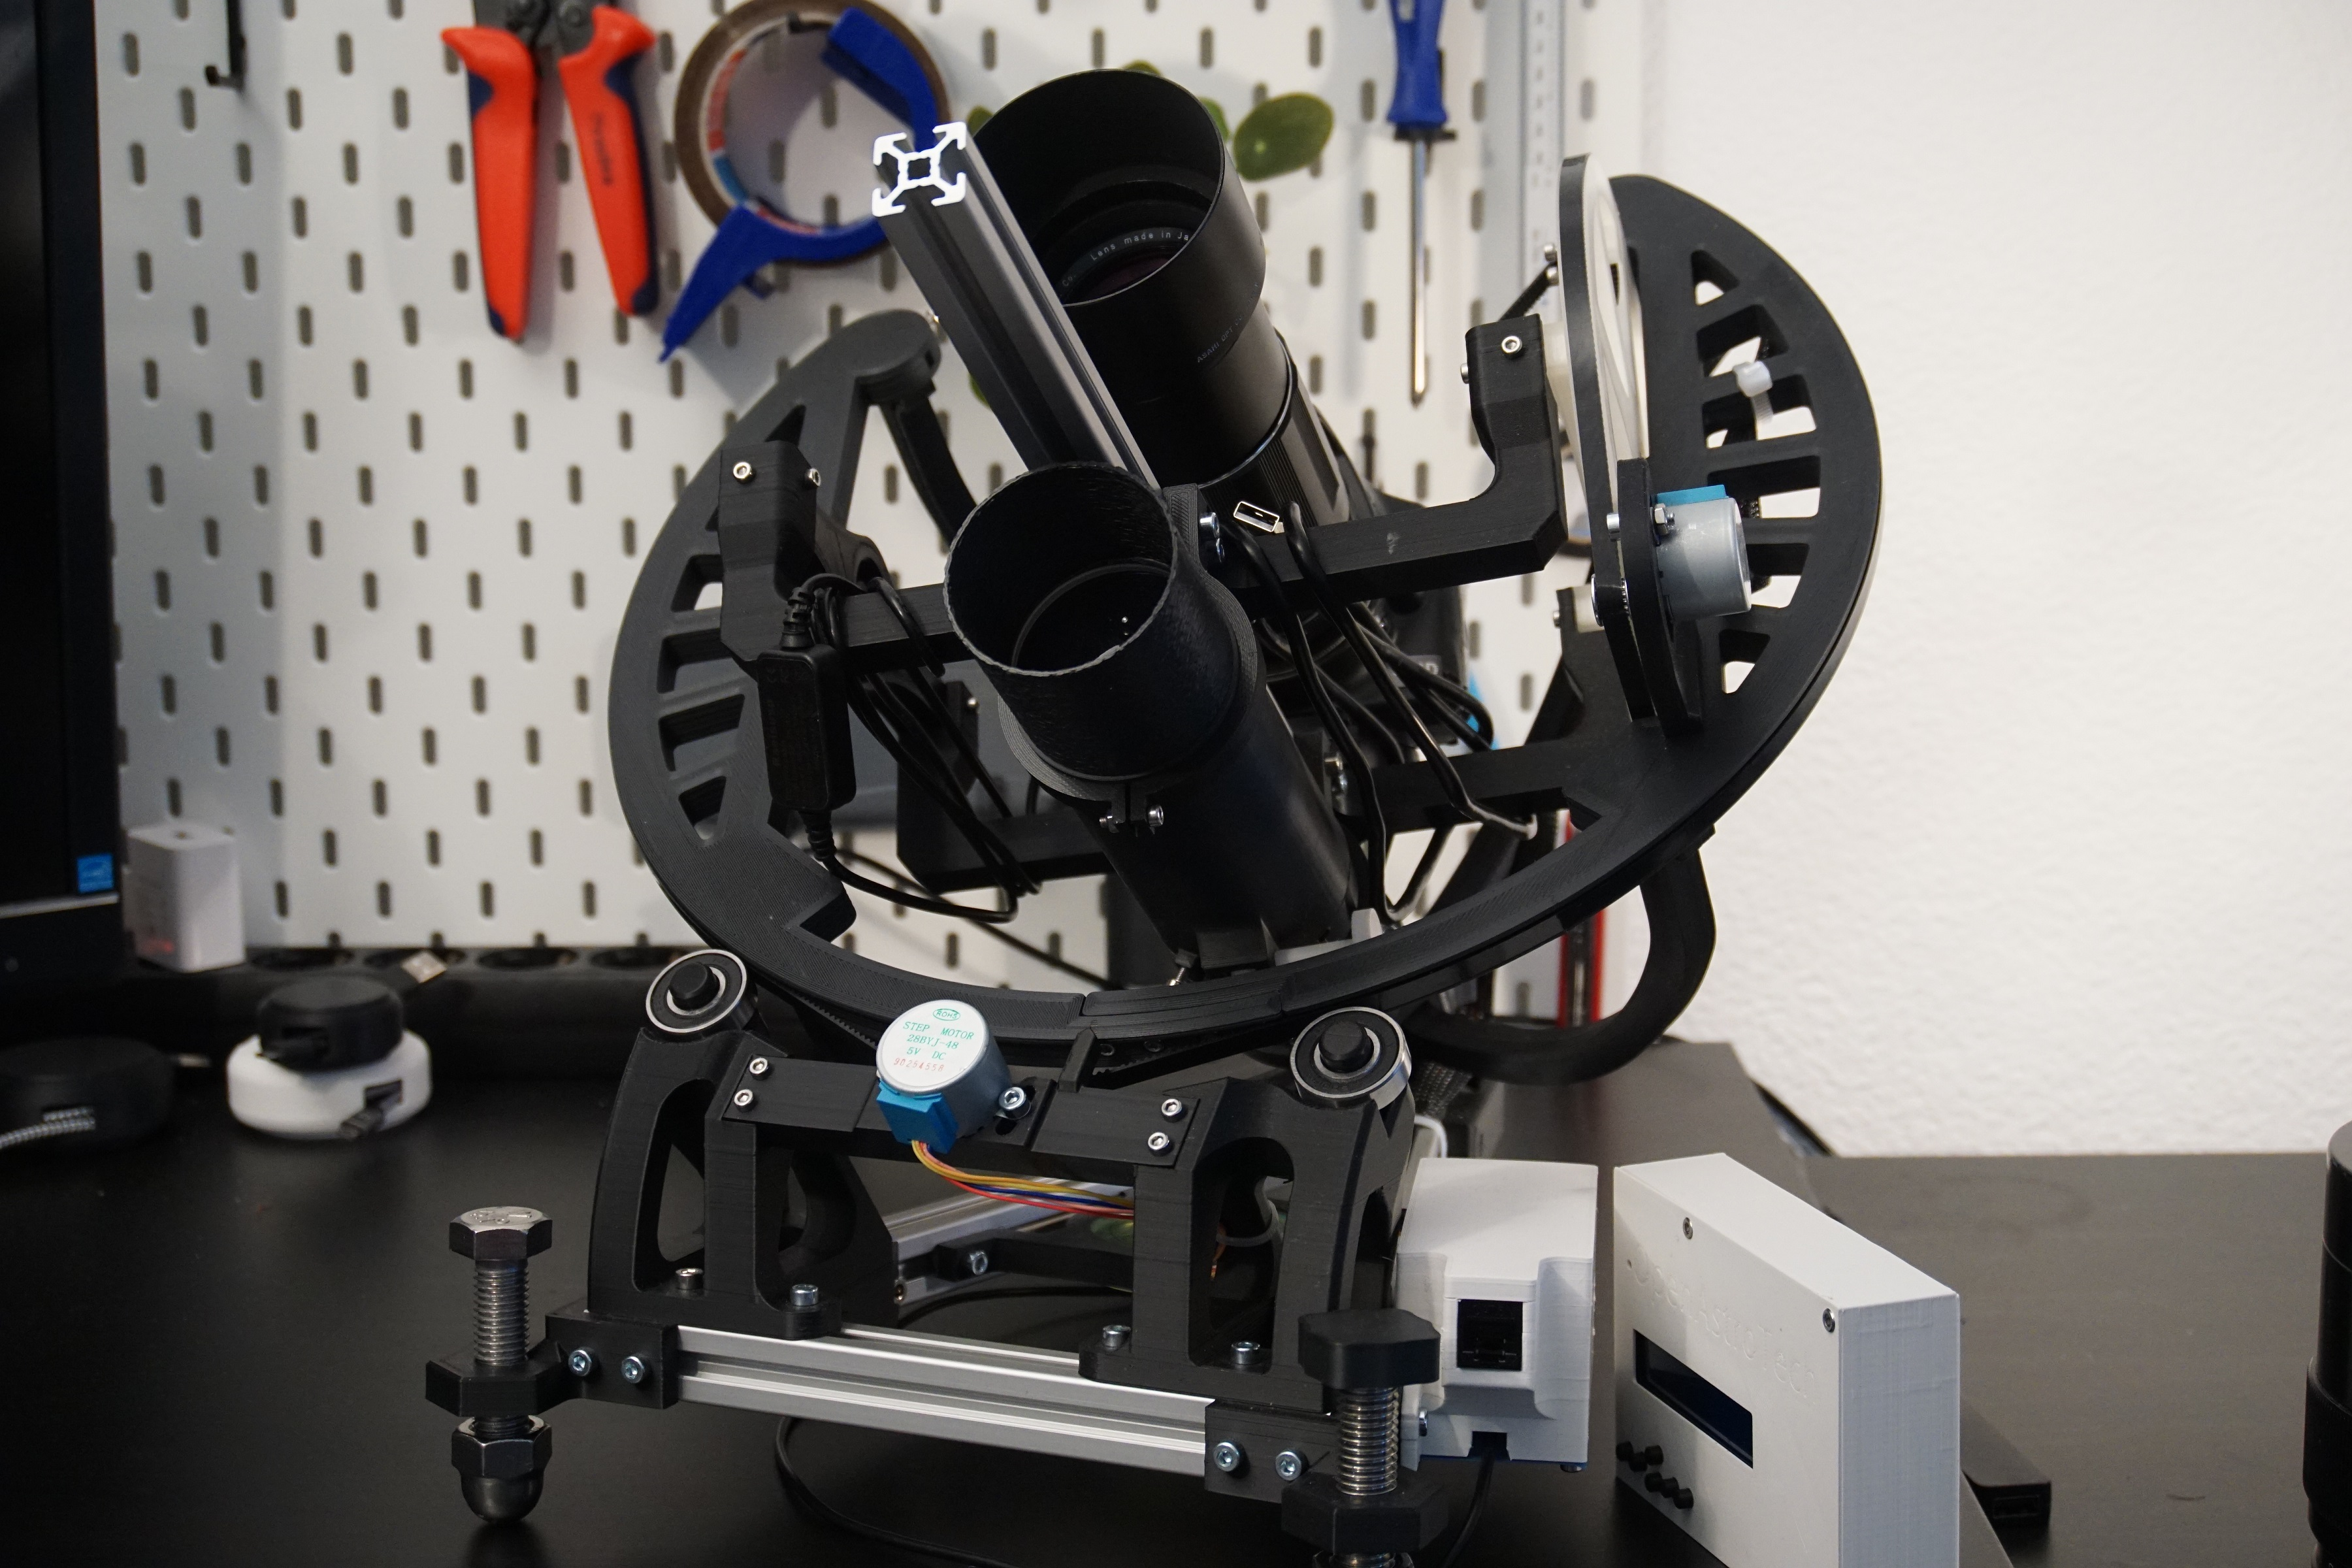
\includegraphics[width=0.7\linewidth]{images/background/openastrotracker.jpeg}
	\caption{OpenAstroTracker, another DIY star tracker.}
\end{figure}

\subsubsection{The OG star tracker}
The \textbf{OG star tracker} \cite{ogstartracker} started and acquired popularity after this project started, so it could not have been considered. This star tracker is a very low-cost solution, can be used with heavy DLSR cameras (up to $3kg$ of payload, and focal length of $300mm$) and is extremely portable. In fact, it fully satisfies the 3 main design goals. What it lacks at the moment is the capability of auto-alignment. 

\begin{figure}[H]
	\centering
	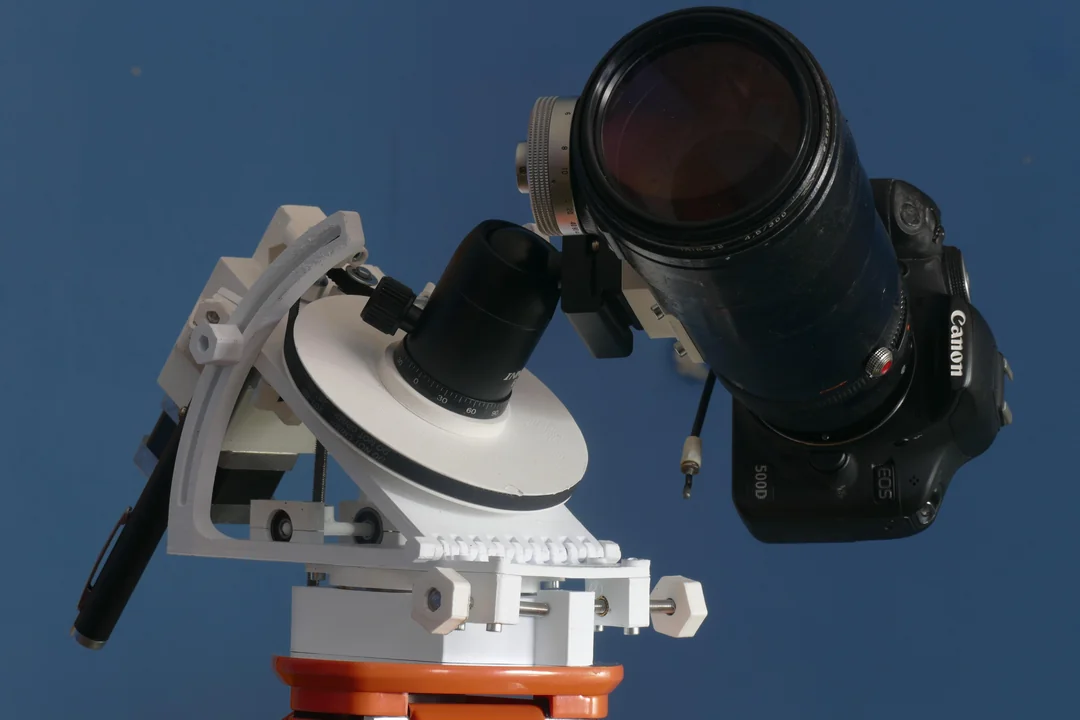
\includegraphics[width=0.7\linewidth]{images/background/ogstartracker.png}
	\caption{The OG Star Tracker, as originally announced on Reddit in the second half of January, 2023 \cite{ogstartrackerreddit}.}
\end{figure}

Since this solution is the most close to the original scope of the project, but it works as intended - unlike my solution, this section will explore more in depth the differences between the two works. 

There are two main differences, which influence the result the most: my experimental solution is based solely on 3D printed gears, which present accuracy problems, while on the OG star tracker only one printed gear was used, and the others are made of metal; furthermore, that projects employs a \textit{gear box}, which can increase very efficiently the output torque utilizing less space, and \textit{drive belts}. 

The second main difference is in the \textit{alignment process}: being completely manual in the OG star tracker, the precision depends only on the human operator; while in this project, it depends on the accuracy and the calibration of the sensors used. This will affect the final results. 

\newpage

\section{Background}\label{sec:intro}

\begin{floatingfigure}[p]{0.35\linewidth}
	\centering
	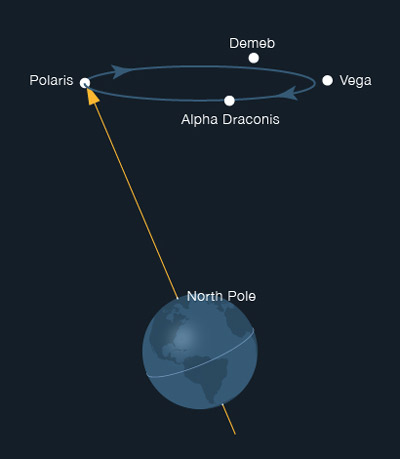
\includegraphics[width=0.35\linewidth]{images/background/2-1-precession-400x4591_nasa.jpg}
	\caption{Polaris is near the Earth's rotation \\}
	\label{fig:polarisnasa}
\end{floatingfigure}	


Before illustrating the details of the developed solution, some technical details about the star tracking process must be understand, in particular why is important to \textbf{align} a star tracker in a certain way. 
\\
\\
The Earth rotates on its axis, with a slight inclination (about 23 degrees) respect to the plane of its revolution around the Sun (its orbit).

Due to this inclination, \textbf{Polaris}, a star also know as the North Star or Pole Star, does not show any movement to the naked eye, since it is very close to Earth's inclination axis. This only works for the northern hemisphere, since Polaris is only visible in this hemisphere. Since Polaris is really bright (relatively speaking), it was also fundamental for navigation. 



All the other stars, on the other hand, that do not lay on the axis, have an apparent movement from east to west. When a camera captures the light from the stars for too long, this movement appears visible \ref{fig:startrail1}. 

While a day on Earth lasts 24 hours, where "day" is defined as the time it takes for the Sun to be visible in the same spot in the sky after the Earth has completed the rotation around his axis, when considering constellation and stars another notion of time should be considered: \textbf{Sidereal Time} \cite{cosmos}. It is the time needed for the "fixed" stars (very distant stars) to appear in the same place on two consecutive nights. This time is shorter than 24 hours by about 4 minutes: 23 hours, 56 minutes and 4.091 seconds. A star tracker needs to perform a complete rotation in the span of sidereal day, not of the 24 hours day. 

\begin{figure}[H]
	\centering
	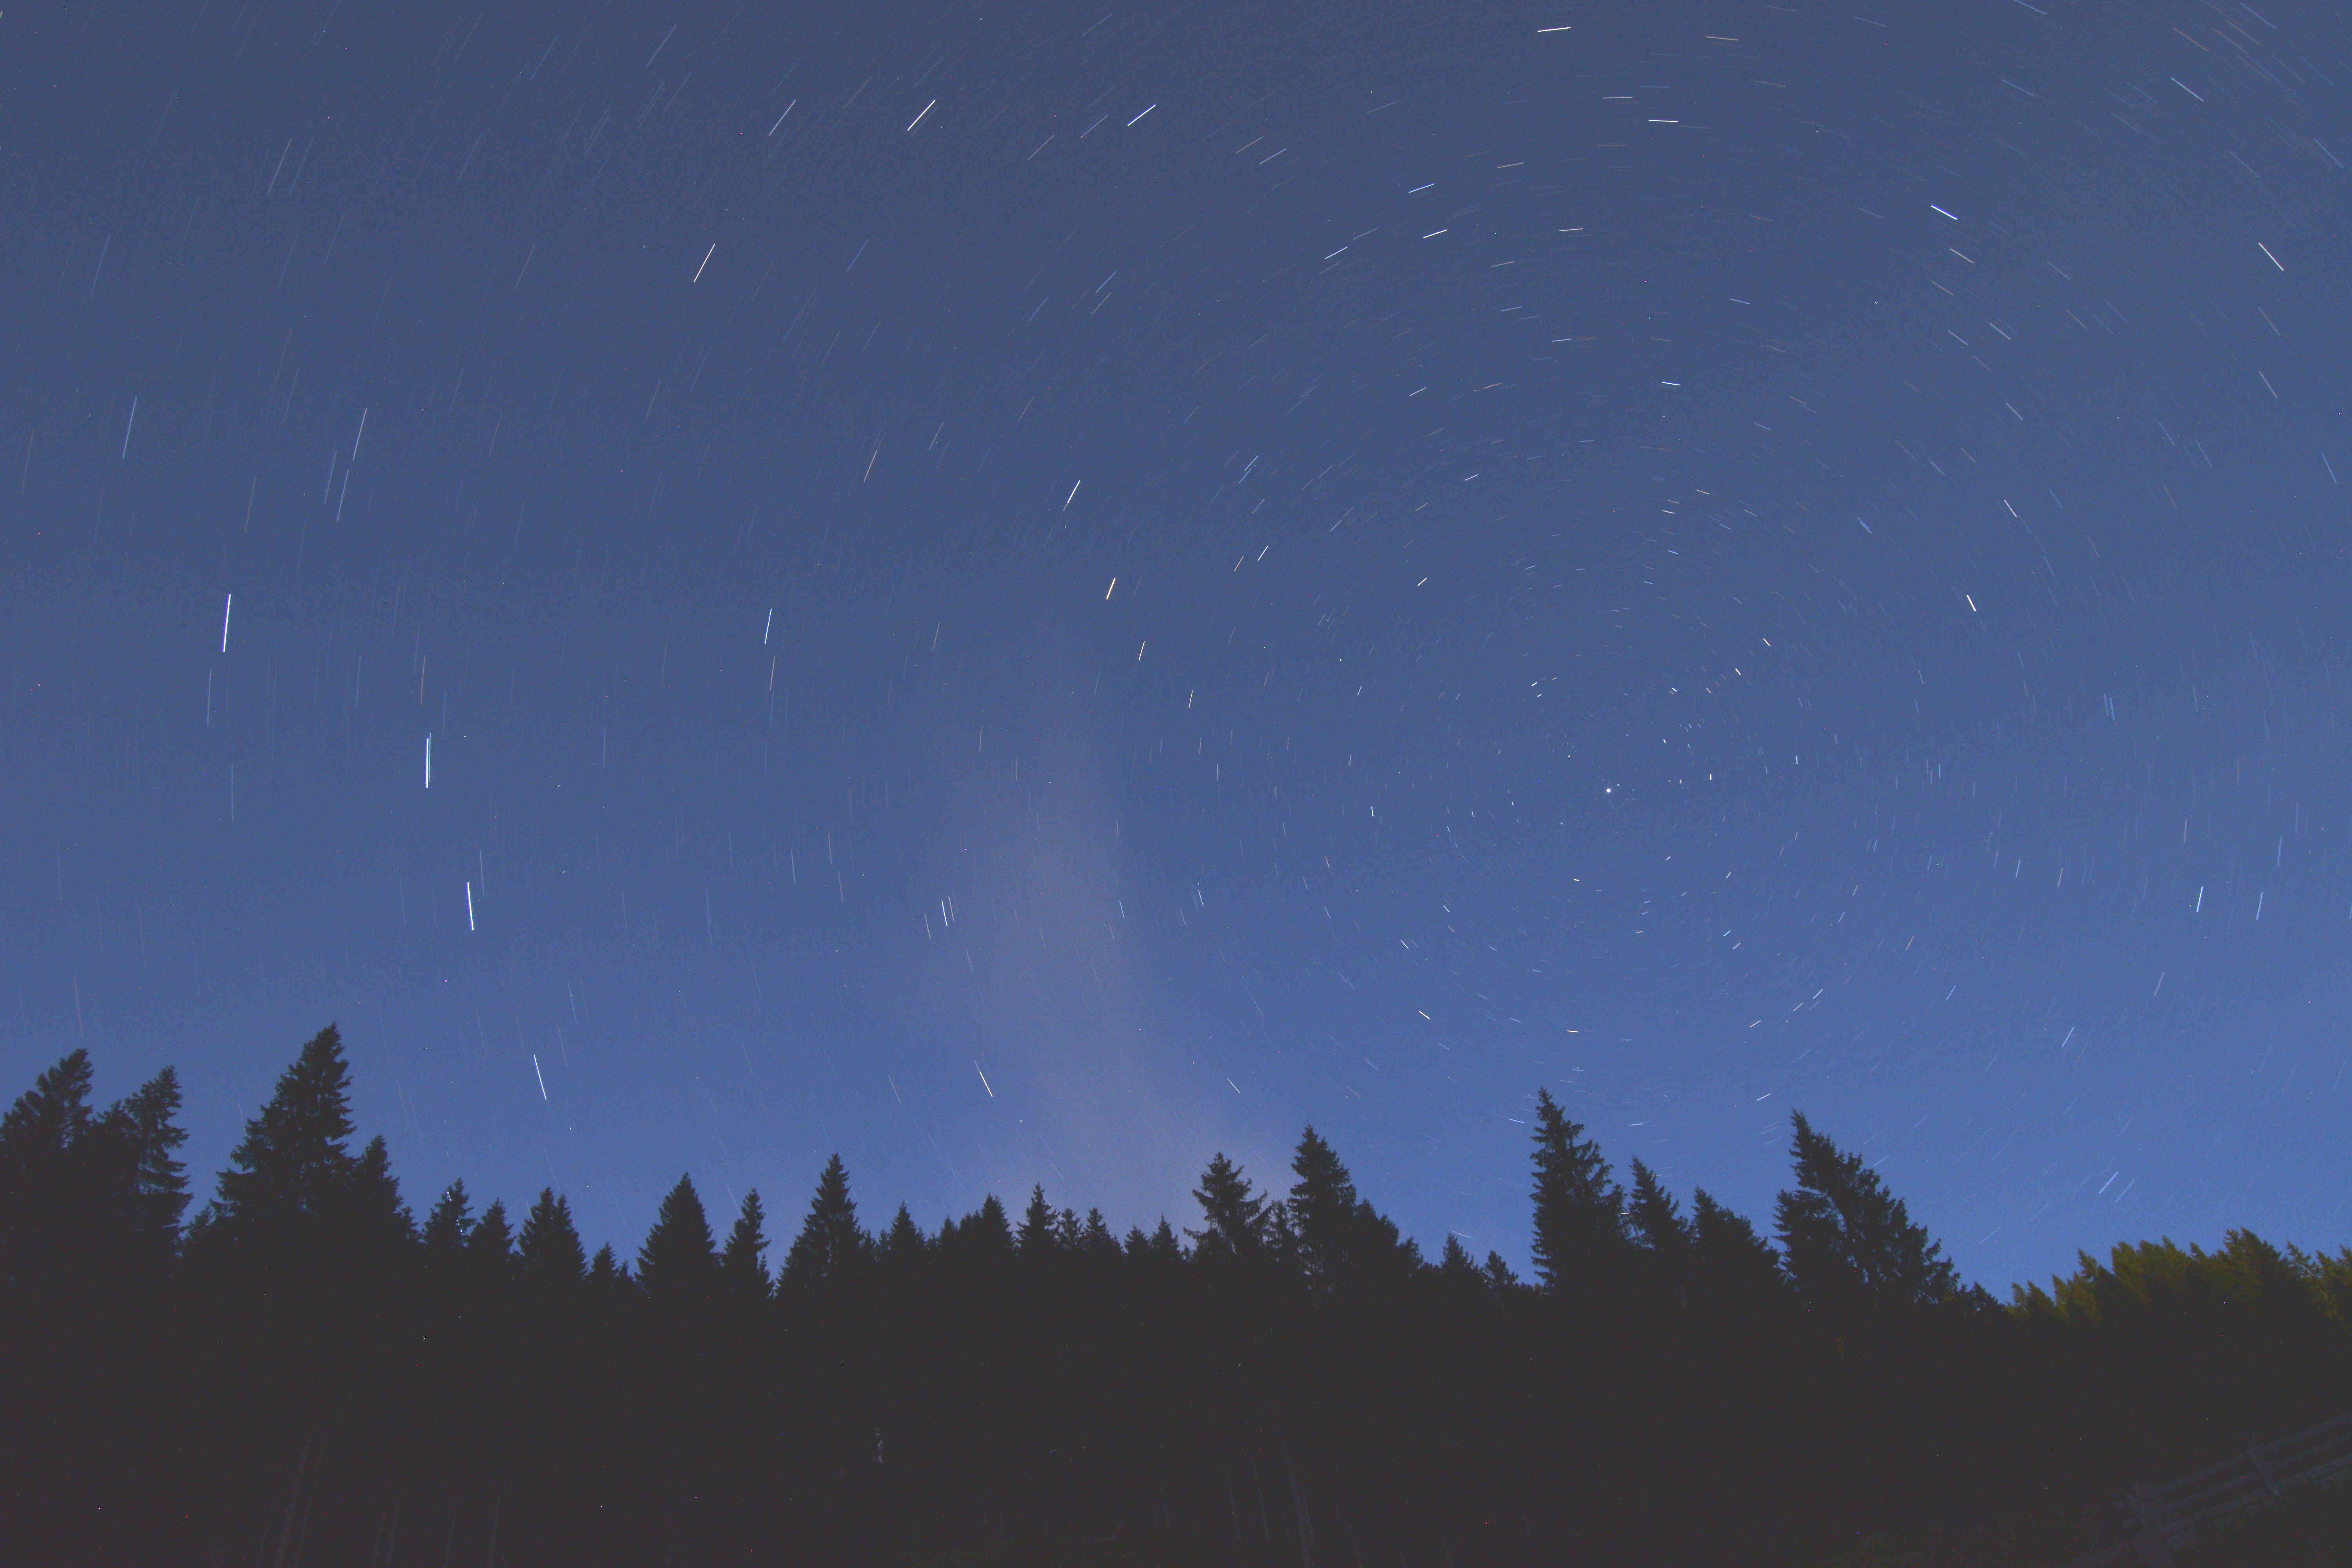
\includegraphics[width=0.7\linewidth]{images/background/startrail}
	\caption{Star trail visible after about 10 minutes of exposure (Polaris is also visible on the right)}
	\label{fig:startrail1}
\end{figure}

\vspace{1em}

\subsection{Camera basics and the 500 rule}
How fast the "star movement" starts to become evident, depends on the lens and the camera specifications. 

The first important factor is called \textbf{focal length}, and, to simplify, is the level of zoom the lens has. So, the bigger the focal lens, the lesser the angle of view will be; and of course also the magnification will be bigger. 

\begin{figure}[H]
	\centering
	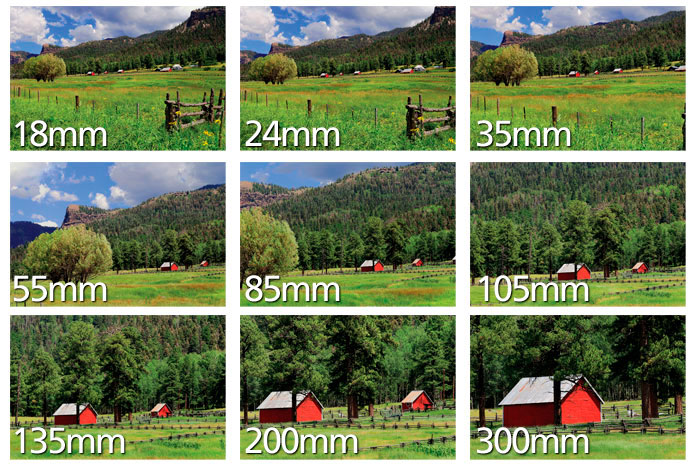
\includegraphics[width=0.7\linewidth]{images/background/focallength}
	\caption{Lens focal length tells us the angle of view - how much of the scene will be captured - and the magnification - how large individual elements will be \cite{nikon}. Notice the difference between 18mm and 300mm.\\}
\end{figure}

When a moving object is magnified, its movement will be "amplified"; this implies that with a greater focal length, the \textit{star trail} effect will appear with less exposure time; on the other hand, with less magnification the object will appear still for longer time. 

Another important element is the \textbf{crop factor}. Before digital, a common film size was 35mm, meaning that an image going through a lens was impressed on a light-sensible film, with a rectangular shape of a certain size (35mm was the size of the film, side to side).

\begin{figure}[H]
	\centering
	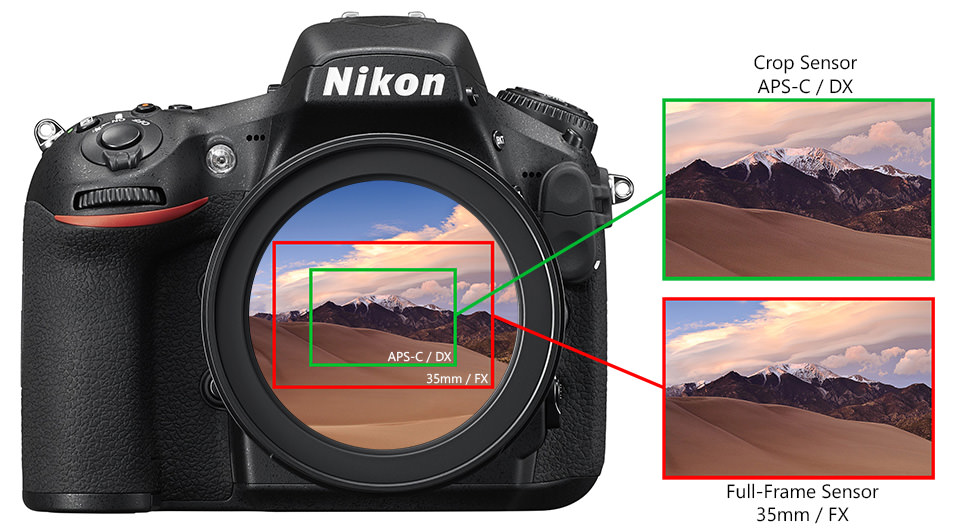
\includegraphics[width=0.7\linewidth]{images/background/crop_factor.jpg}
	\caption{Crop factor visualization \cite{cropfactor}: a Full-Frame vs APS-C Sensor size are compared.\\}
\end{figure}

With digital, sensor sizes changed, and the same image passing though the lens now can hit a different amount of space, depending on the size of the underlying sensor, so the final image is "cropped" respect to a 35mm film. 

There are different common standard sizes for digital camera sensors, but we will refer to the APS-C size, wich has a crop factor of 1.5. The crop factor is the ratio of sensor size to the 35mm, and helps lens manufacturer and photographers understand what the final field of view of the camera will be. 

After having introduced these two concepts, focal length and crop factor, it is possible to introduce the \textbf{500 rule}  \cite{500rule}. This is an empirical rule to compute the maximum exposure time usable before the star trail effect appears. 



The rule can be expressed as:

$$ SS = \frac{500}{CF \cdot FL}$$

where $SS$ is the exposure time, or \textit{shutter speed}, $CF$ is the crop factor and $FL$ is the focal length. The graph \ref{pic:500graph} shows the shutter speed for different focal lengths, and a crop factor of 1.5:
\\
\\
\begin{figure}[H]
	\centering
	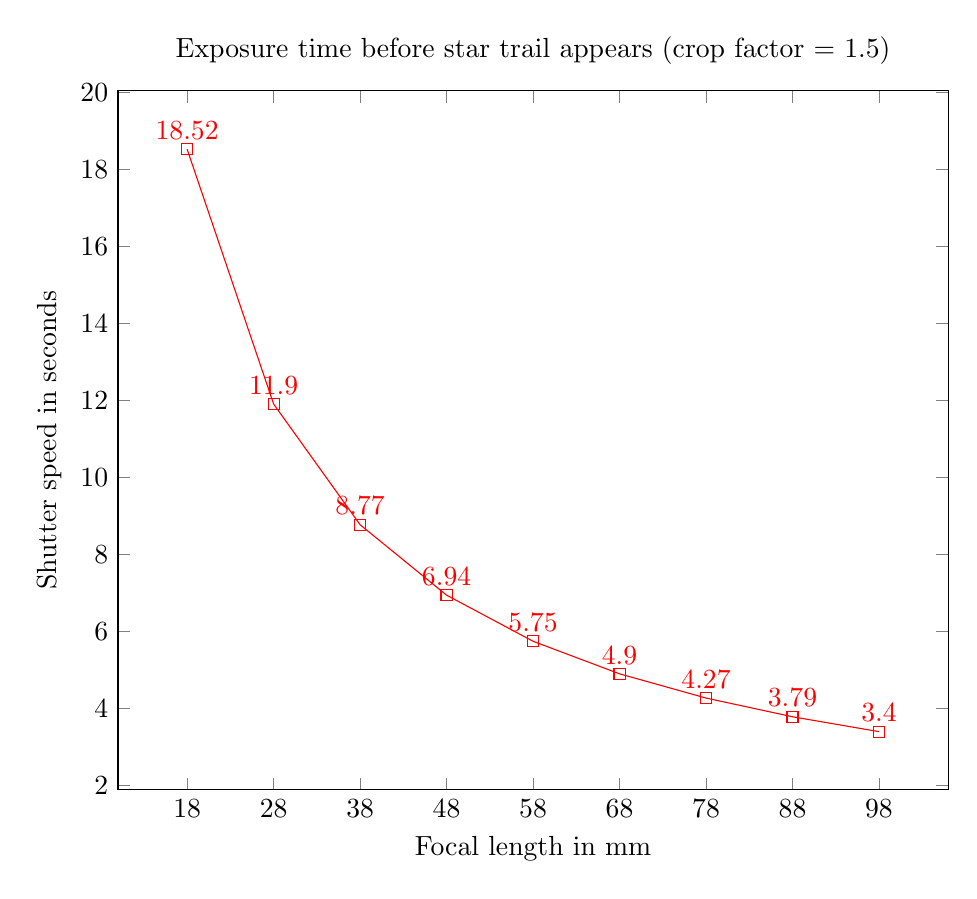
\begin{tikzpicture}
		\begin{axis}[
			width=\textwidth,
	  		title={Exposure time before star trail appears (crop factor = 1.5)},
			xlabel={Focal length in mm},
			ylabel={Shutter speed in seconds},
			xtick={18, 28, 38, 48, 58, 68, 78, 88, 98},
			]
			\addplot [ 
			domain=18:98, 
			color=red,
			mark=square, 
			samples = 9,
			nodes near coords, 
			xtick={18, 28, 38, 48, 58, 68, 78, 88, 98},
			]
			{500/(1.5*x)};
		\end{axis}
	\end{tikzpicture}
	\caption{This graph shows the shutter speed computed through the 500 rule. Increasing the focal length (from 18mm to more than 90), the exposure time for a shot without trail decreases.}
	\label{pic:500graph}
\end{figure}

\iffalse
\subsubsection{Right Ascension and Declination}
Since Polaris is not exactly on the Earth's rotation axis, other important concepts are right ascension and declination.  

Every point on Earth can be localized through two coordinates, \textbf{latitude} and \textbf{longitude}, which are respectively the distance in degrees north or south of the equator, and the distance in degrees east or west of the prime meridian\footnote{The prime meridian is the imaginary line connecting the poles and passing through Greenwich.}. 

\begin{figure}[H]
	\centering
	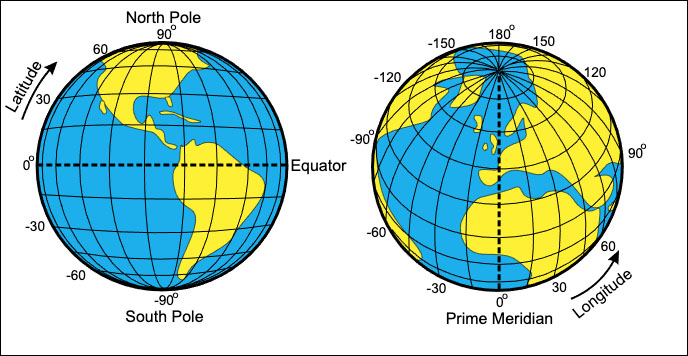
\includegraphics[width=0.5\linewidth]{images/background/RA-Dec-Latitude-longitude-wiki-public-domain-cc1.0}
	\caption{Earth is shown covered in an imaginary grid of latitude lines (measured from $0^{\circ}$ to $90^{\circ}$ north and south of the equator) and longitudes lines (measured from $0^{\circ}$ to $180^{\circ}$ east and west of the prime meridian).}
	\label{fig:latlon}
\end{figure}

Right ascension and declination are the coordinates of celestial objects: declination corresponds to latitude, and right ascension to longitude. To accurately find a celestial object, like Polaris, is very useful to know these coordinates. 

\begin{figure}[H]
	\centering
	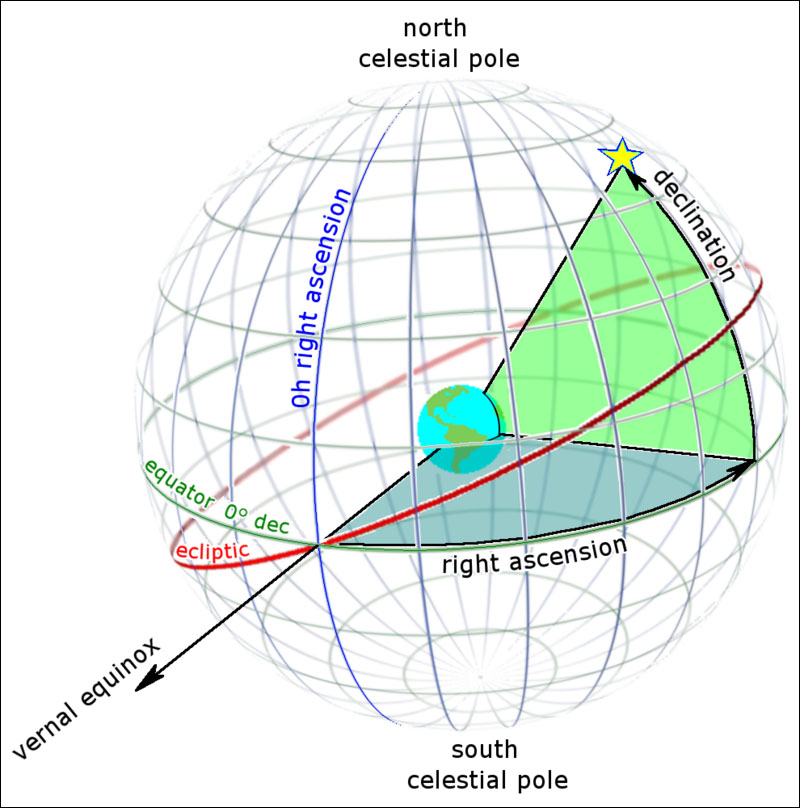
\includegraphics[width=0.5\linewidth]{images/background/RA-Dec-wiki-Tom-RuenCC-BY-SA-3.0.jpg}
	\caption{Declination (green) is measured in degrees north and south of the celestial equator. Right ascension, akin to longitude, is measured east from the equinox. The red circle is the Sun's apparent path around the sky, which defines the ecliptic.}
	\label{fig:radec}
\end{figure}

Earth's equator, at $ 0^{\circ} $ latitude, becomes also the
 \textit{celestial equator};   declination is measured in degrees: e.g. Polaris has a declination of $ +89^{\circ}  15^{\prime} $. 

The right ascension is slightly more complicated. The $0^{\circ}$ mark in the sky separating the east form the west is placed at the \textbf{vernal equinox}. This is the spot where the sun arrives on the first day of spring. But right ascension is measured in hours: the sky can be treated as a clock, since it wheels by as Earth rotates. And ascension is also measured in one direction, east. There are 24 lines for the right ascension hours, as a day on the Earth lasts 24 hours. Polaris has a right ascension of $2^h 41^m$.

\begin{figure}[h!]
	\centering
	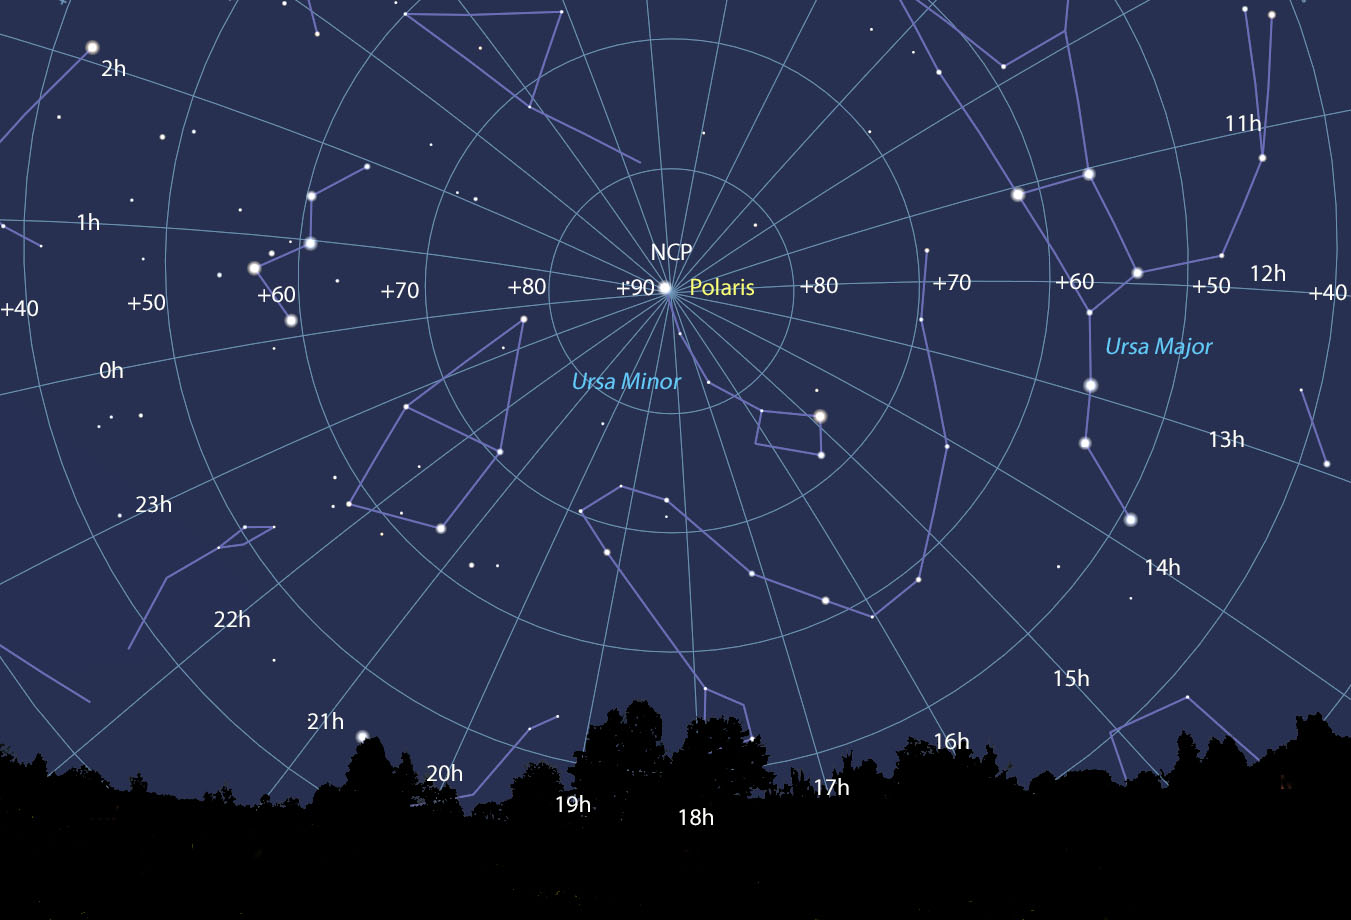
\includegraphics[width=0.5\linewidth]{images/background/RA-Dec-celestial-pole.jpg}
	\caption{This view shows the north celestial pole (NCP) and polar regions. Declinations are labeled every 10° and the hours of right ascension are shown around the circle. By convention, 0h is used instead of 24h. 
		\textit{Stellarium}}
	\label{fig:stellarium}
\end{figure}
\fi 

\subsection{Magnetic declination} \label{sec:mag_decl}
\begin{floatingfigure}[r]{0.4\linewidth}
	\centering
	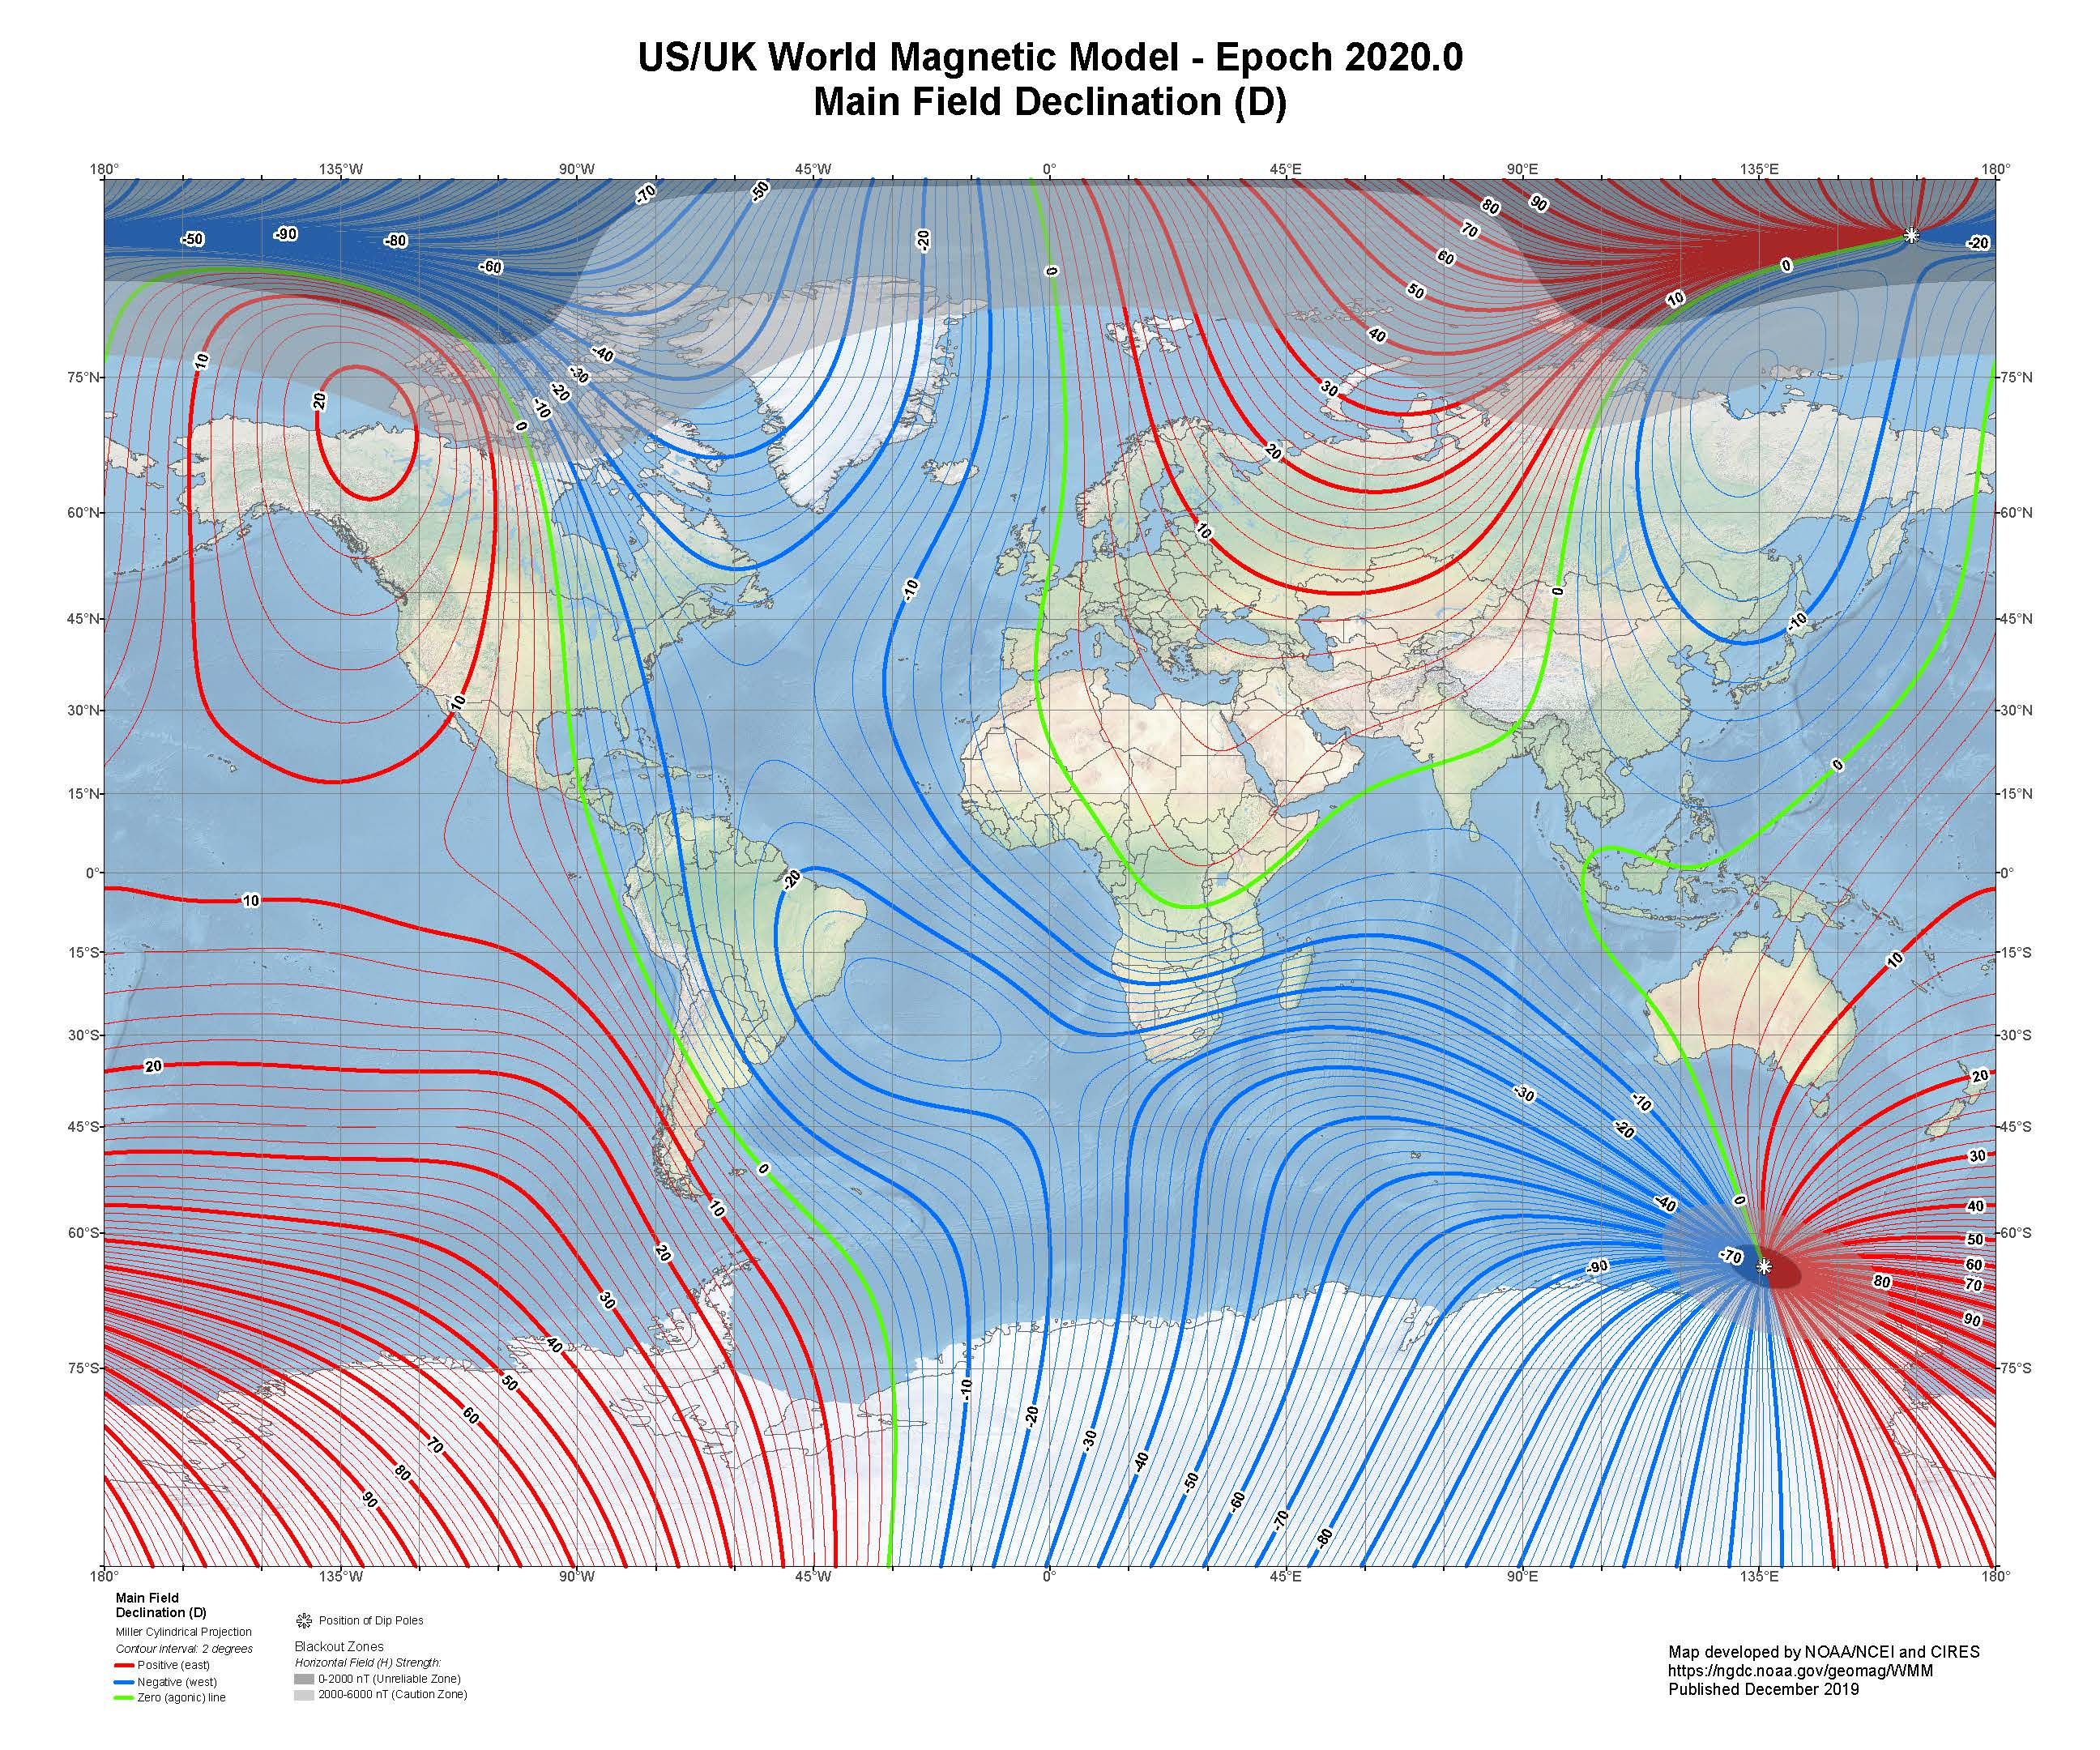
\includegraphics[width=0.37\linewidth]{images/background/wmm2020model.jpg}
	\caption{The WMM2020 declination projection \cite{wmm2020}. The declination is considered positive when the angle measured is \textcolor{red}{east} (red lines) of true north and negative when \textcolor{blue}{west} (blue lines).\\}
\end{floatingfigure}

The Earth has a magnetic field; but this is not uniform across the globe. It even changes with time \cite{magndecl}

Hence, compasses can only point towards the \textbf{magnetic north}, which can vary from place to place, and not to the \textbf{geographic north}. 

The magnetic field - and the magnetic north - forms an angle with the geographic north; this angle is called \textbf{magnetic declination}. 

It is possible to compute in advance and know how much this angle is, given the position and the time. \textbf{The World Magnetic Model} \cite{wmm2020} is the standard model used in navigation to account for the magnetic declination. This model is produced at 5-year intervals, with the current model expiring on December 31, 2024.
\\
\subsection{Polar alignment}
Now it is possible to put together all the concepts previously presented. 

The idea behind star tracking is to move the camera according to the rotation of the Earth, in order to compensate for this movement. To achieve this, a star tracker needs to rotate very slowly  - a complete rotation has to happen in a sidereal day time   - in the same way and speed as the stars seem to move, from east to west. Furthermore, a star tracker needs to be aligned with the axis of the movement, which is the rotational axis of the Earth. 

This is accomplished trough \textbf{polar alignment}: the star tracker needs to be aligned with the Earth's rotational axis, which is achieved when the star tracker points to Polaris \cite{polaralignment}. If great precision is required, e.g. when we want to use a big focal length, then an exactly alignment is absolutely necessary; but when there is no such requirement, pointing towards Polaris should be sufficient.

\begin{figure}[H]
	\centering
	\subfigure[Polar drift]{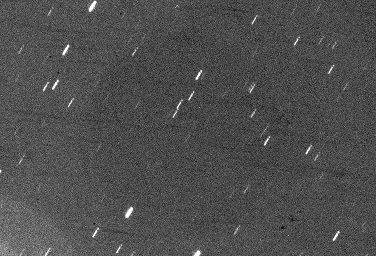
\includegraphics[width=0.45\linewidth]{images/background/mount_west_1}}
	\subfigure[Field rotation]{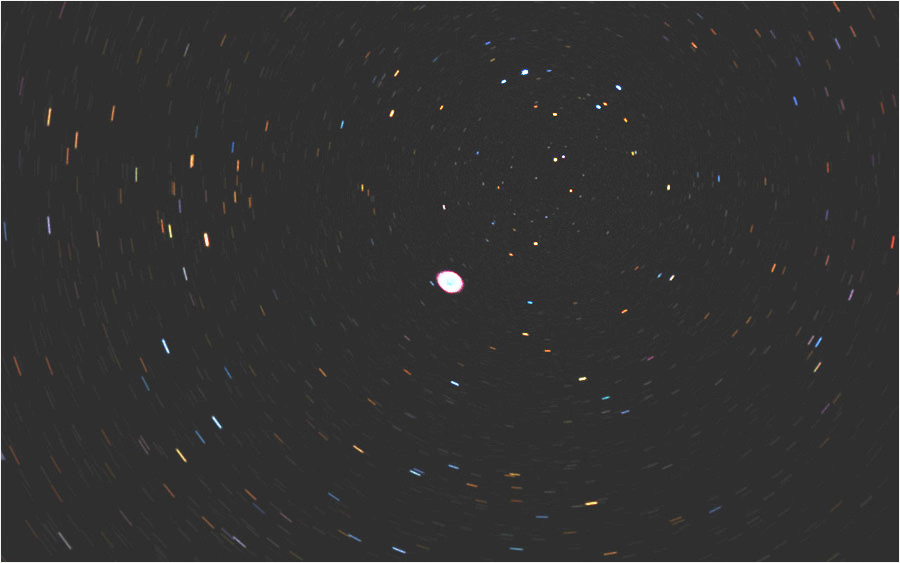
\includegraphics[width=0.45\linewidth]{images/background/trails_04}}
	\caption{Examples of misalignment. The first is a case of general \textit{polar drift} \cite{drift}: the mount was adjusted a small amount west and above the pole; the second is a case of \textit{field rotation} \cite{fieldrotation}: the stars seems to rotate around the guide star in the field.\\}
	
\end{figure}

While it is possible to exactly point Polaris with a special scope, called the \textit{polar scope}, its position can be determined by knowing the observer's latitude and where the geographic north is: in fact, as previously discussed, Polaris is above Earth's rotation axis, which passes through the poles, so Polaris is above the North Pole. The latitude is useful to know how many degrees to look up above the horizon to find the star: for example, an observer located at $ +44^{\circ}  15^{\prime} $ should point towards north and look up around $ 44^{\circ}$ from the ground. 
\\
\\
Finally, there is a type of mounting mechanism that allow to rotate a telescope or camera to track the movement of the stars: an \textbf{equatorial mount}. These are designed more specifically for astrophotography, since allow for longer exposure time. There is another type of mount to observe the sky with a telescope or a camera, an \textbf{alt-azimuth} mount: this is a slightly simpler mechanism, but it doesn't allow for long exposure time, so it is not suitable for astrophotography. 

As previously discussed, an equatorial mount needs to be aligned with Polaris in the most precise way possible; the camera is then mounted on top and it rotates as required. 


\section{Design of the star tracker}
After discussing what the requirements for the project are, and some background in astrophotography, the following sections provide implementation details. 

This section is about the case for the various components, such as sensor, motors and battery. 

All the case components were developed using a cad software, \textbf{FreeCAD} and printed using a 3D printer, the \textbf{Creality Ender 3 Pro}. The material used is \textbf{PLA}. 
 
While the use of this technique introduces stability and precision problems, it is really cheap and quick to build simple prototypes. This affects in some ways  the final result, but for an "experiment" such as this one is more than suitable. 

There are also some minor errors such as wrong holes dimension, that were not corrected because it required reprinting entire parts; since these errors do not compromise the final build, were corrected with traditional tools (such as sandpaper), require a waste of time and material to reprint the corrected part and in general are not relevant to the design of the star tracker, they are omitted in the rest of the report. 
\\
\\
The star tracker is an \textbf{equatorial mount}, has a hole at the bottom to be mounted on a tripod and is composed of three parts, which will be referred as \textit{base}, \textit{middle} and \textit{top}. 

Details about the electric and electronic components will be omitted in this section, to be discussed thoroughly in the next section.  

\subsection{Base}
The base of the star tracker is a cube and it fits:
\begin{itemize}
	\item a \textbf{Raspberry Pi 3B+}: performs all the computation;
	\item the \textbf{input system}: button, led and a switch
	\item a \textbf{battery}: it powers all the motors
	\item a \textbf{gps} sensor and its \textbf{antenna}
	\item two \textbf{DC-DC} converters
	\item a \textbf{battery charger circuit}
	\item two \textbf{motor drivers}
	\item a \textbf{stepper motor}
	\item a \textbf{intermediate section} composed of: 
	\subitem{-} a \textbf{flat surface}, to separate all the previous components 
	\subitem{-} two \textbf{gears} that rest on the surface, to rotate the \textit{middle} part
	\item a \textbf{lid}, to close the cube
\end{itemize}

On the bottom of this cube there is a \textit{1/4 inch threaded hole}, which is the standard format for photographic screws: this allows the base to be mounted on any standard tripod. The base was also printed with some "missing" parts on the bottom, to reduce the material required for the print; in the inner side of the bottom, there are some empty cylinders to screw some of the components; other holes are on the side of the cube, and the relative components are keep in place vertically.



\begin{figure}[H]
	\centering
	\subfigure[Bottom]
		{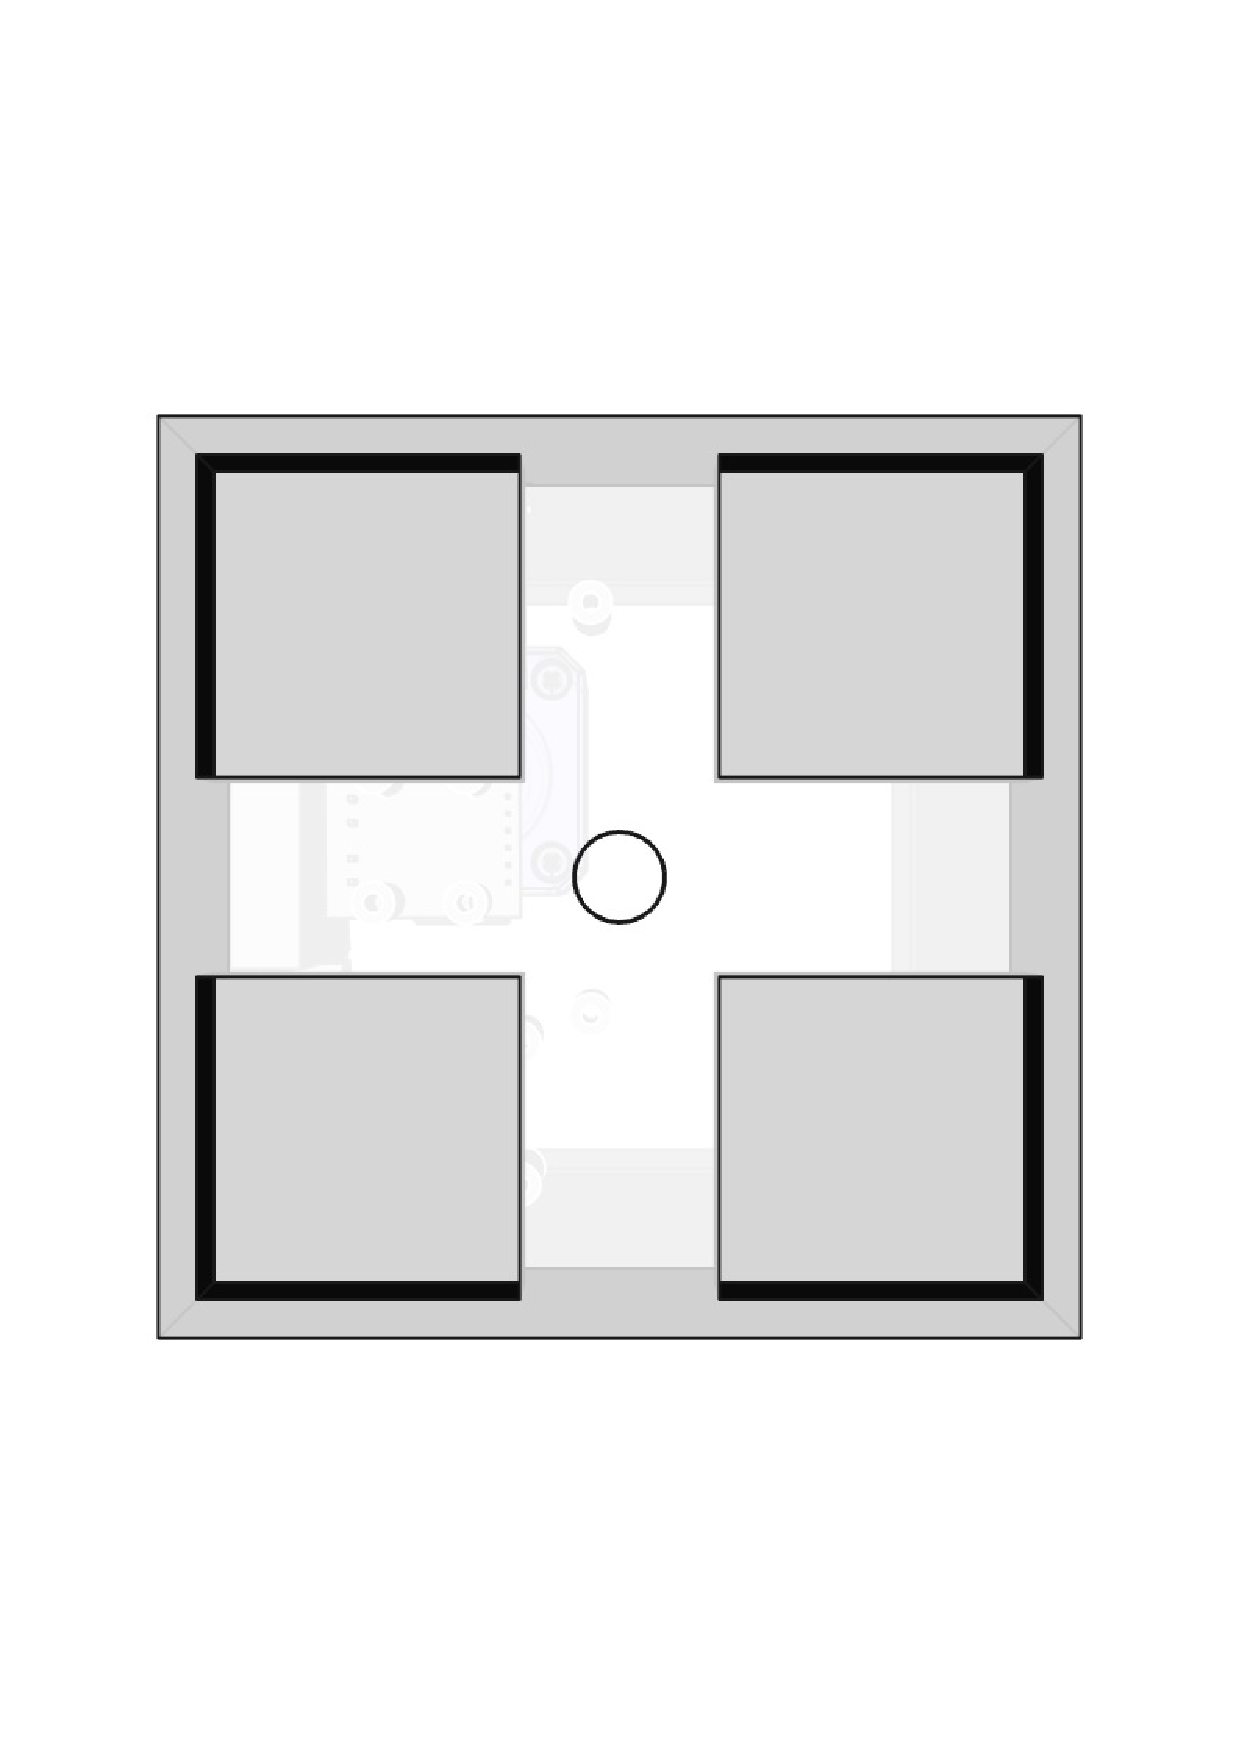
\includegraphics[width=0.45\linewidth]{images/design/base/base_bottom}}
	\subfigure[Side]
		{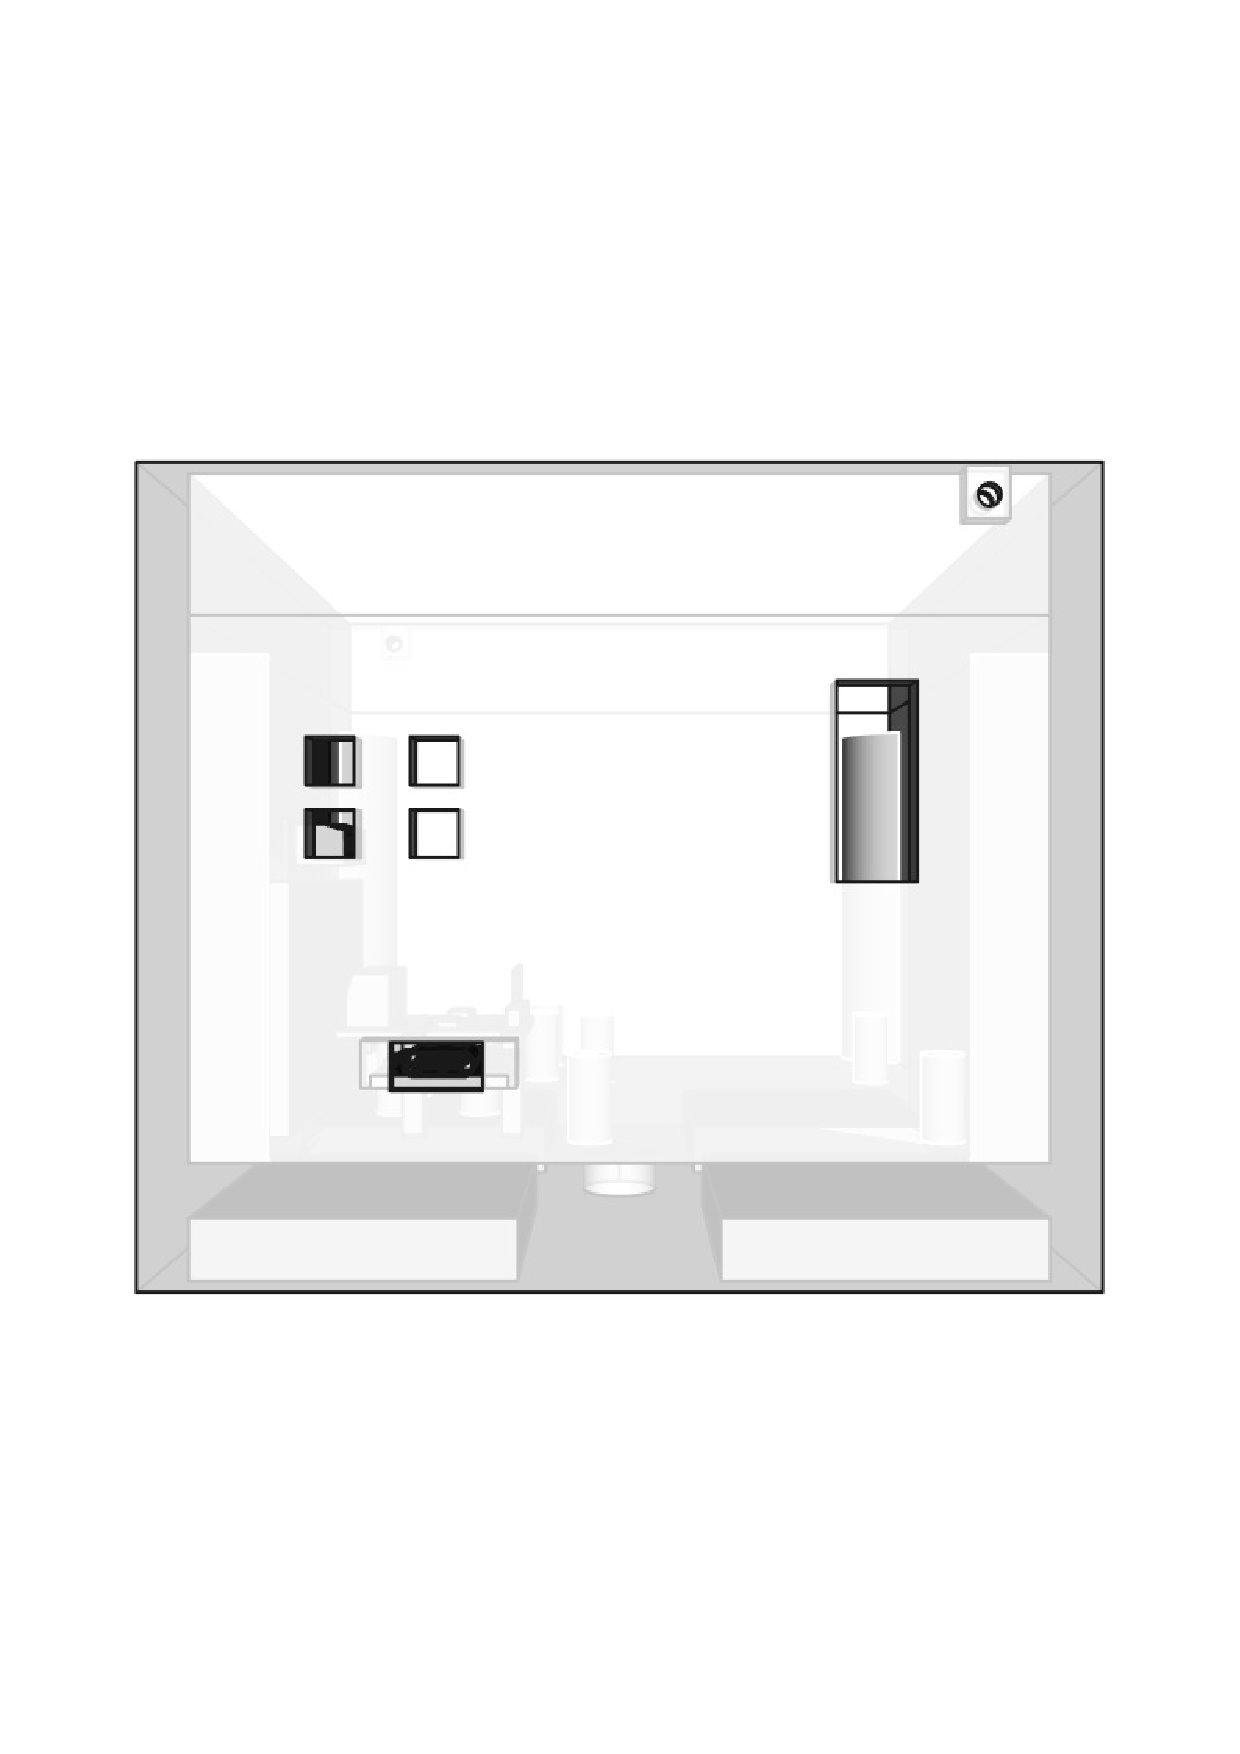
\includegraphics[width=0.45\linewidth]{images/design/base/base_input}}
	
	\caption[Bottom of the base]{(a) is the bottom of the base; it is visible the hole for the photographic screw. In (b), on the side, the holes are for led, buttons, a switch and a recharge circuit. }
	\label{fig:basecolumns}
\end{figure}


In the inner of the cube there are four "columns", on the vertexes: it allows the flat surface to be screwed inside the cube, on the top of these columns. 

\begin{figure}[H]
	\centering
	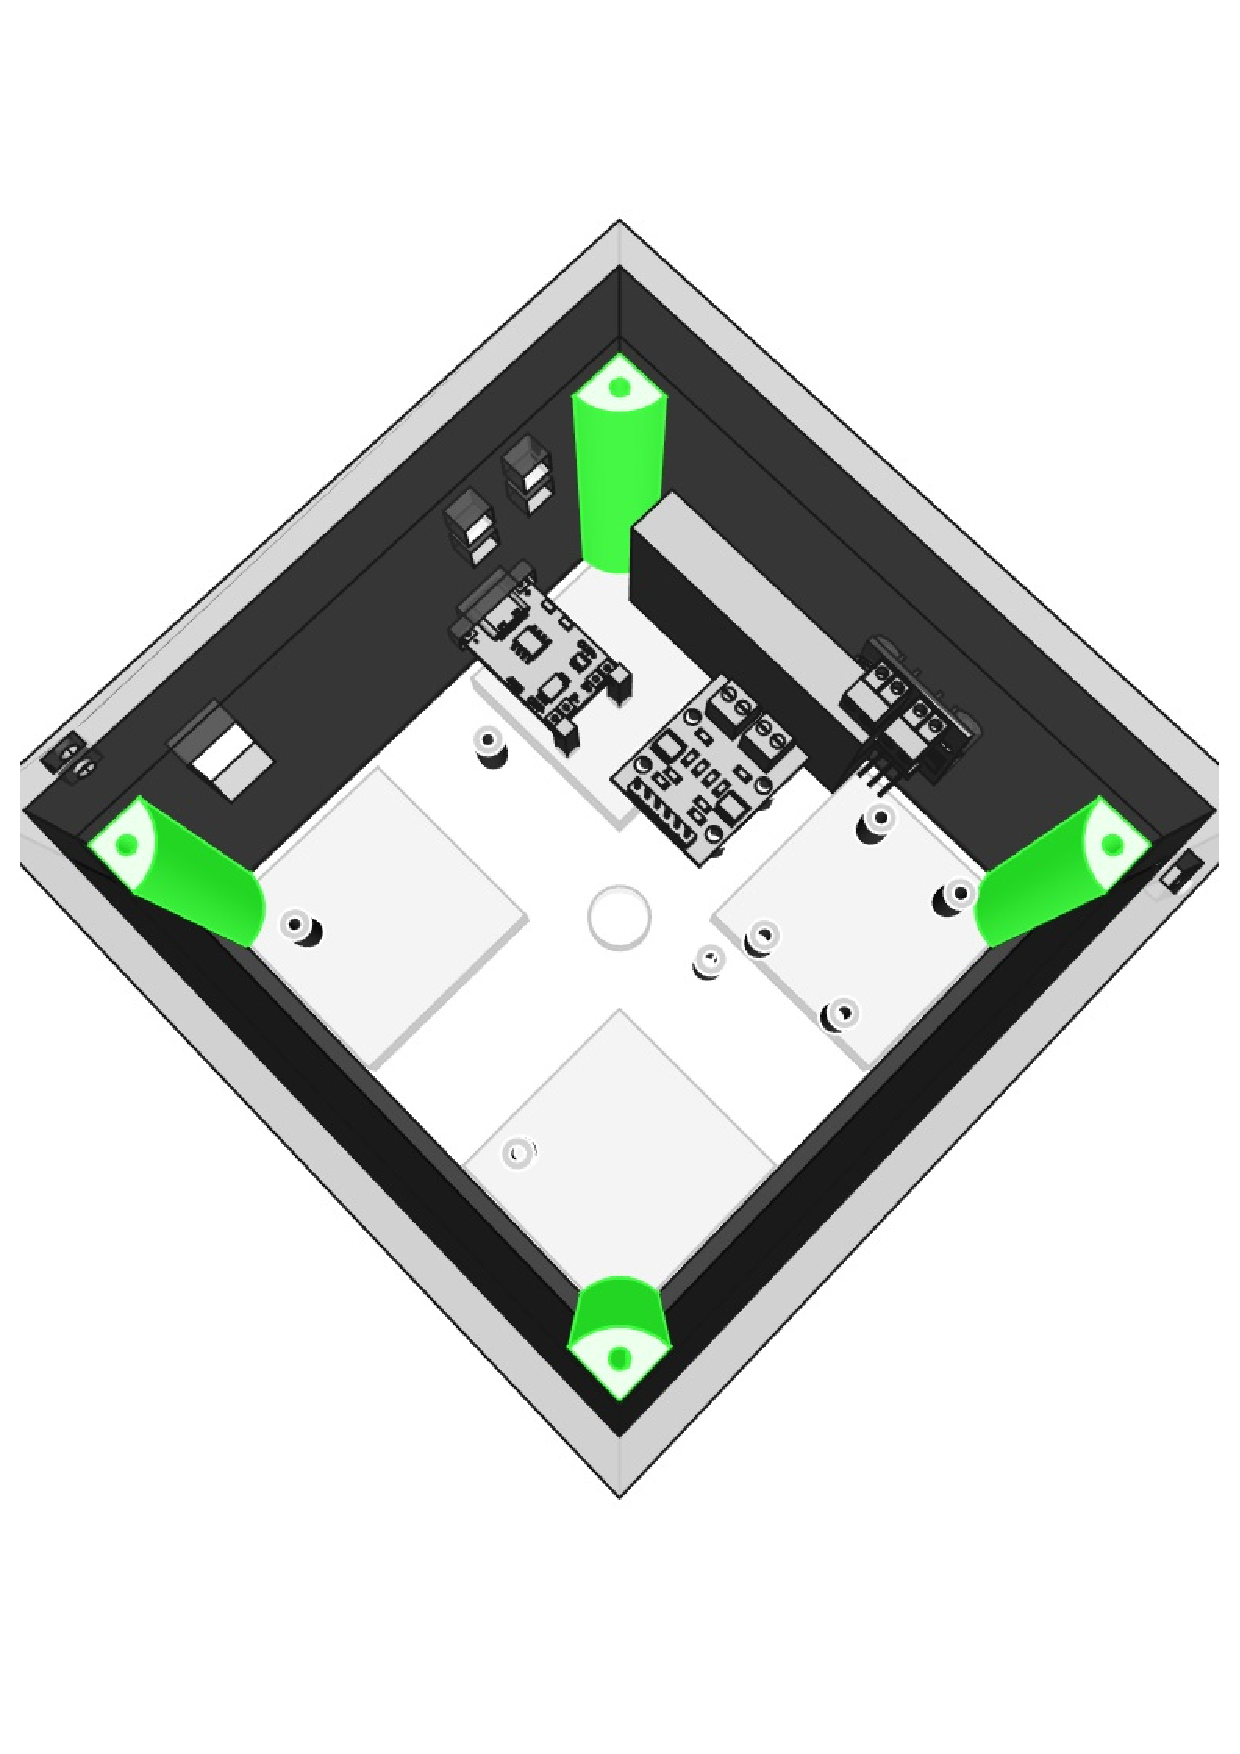
\includegraphics[trim=0 100 0 100 , clip,  width=0.5\linewidth]{images/design/base/base_columns}
	\caption[Bottom of the base]{The green elements are the columns where the flat surface is screwed. There are also visible the little cylinders to screw the components such as the Raspberry.}
	\label{fig:basebottom}
\end{figure}

On the side, there are the holes for the user input (and output) system: the four little squares were intended for two led and two buttons, although only one for each is used,  the big rectangle is for the switch and the lower one is for the recharge circuit. 

On the flat surface, at its centre, there is an \textbf{empty cylinder}: this allows all the cables to pass through the centre of rotation of the middle part, and reduces the possibility of \textbf{twisting} the cables rotating the middle. 

\begin{figure}[H]
	\subfigure[flat surface]
		{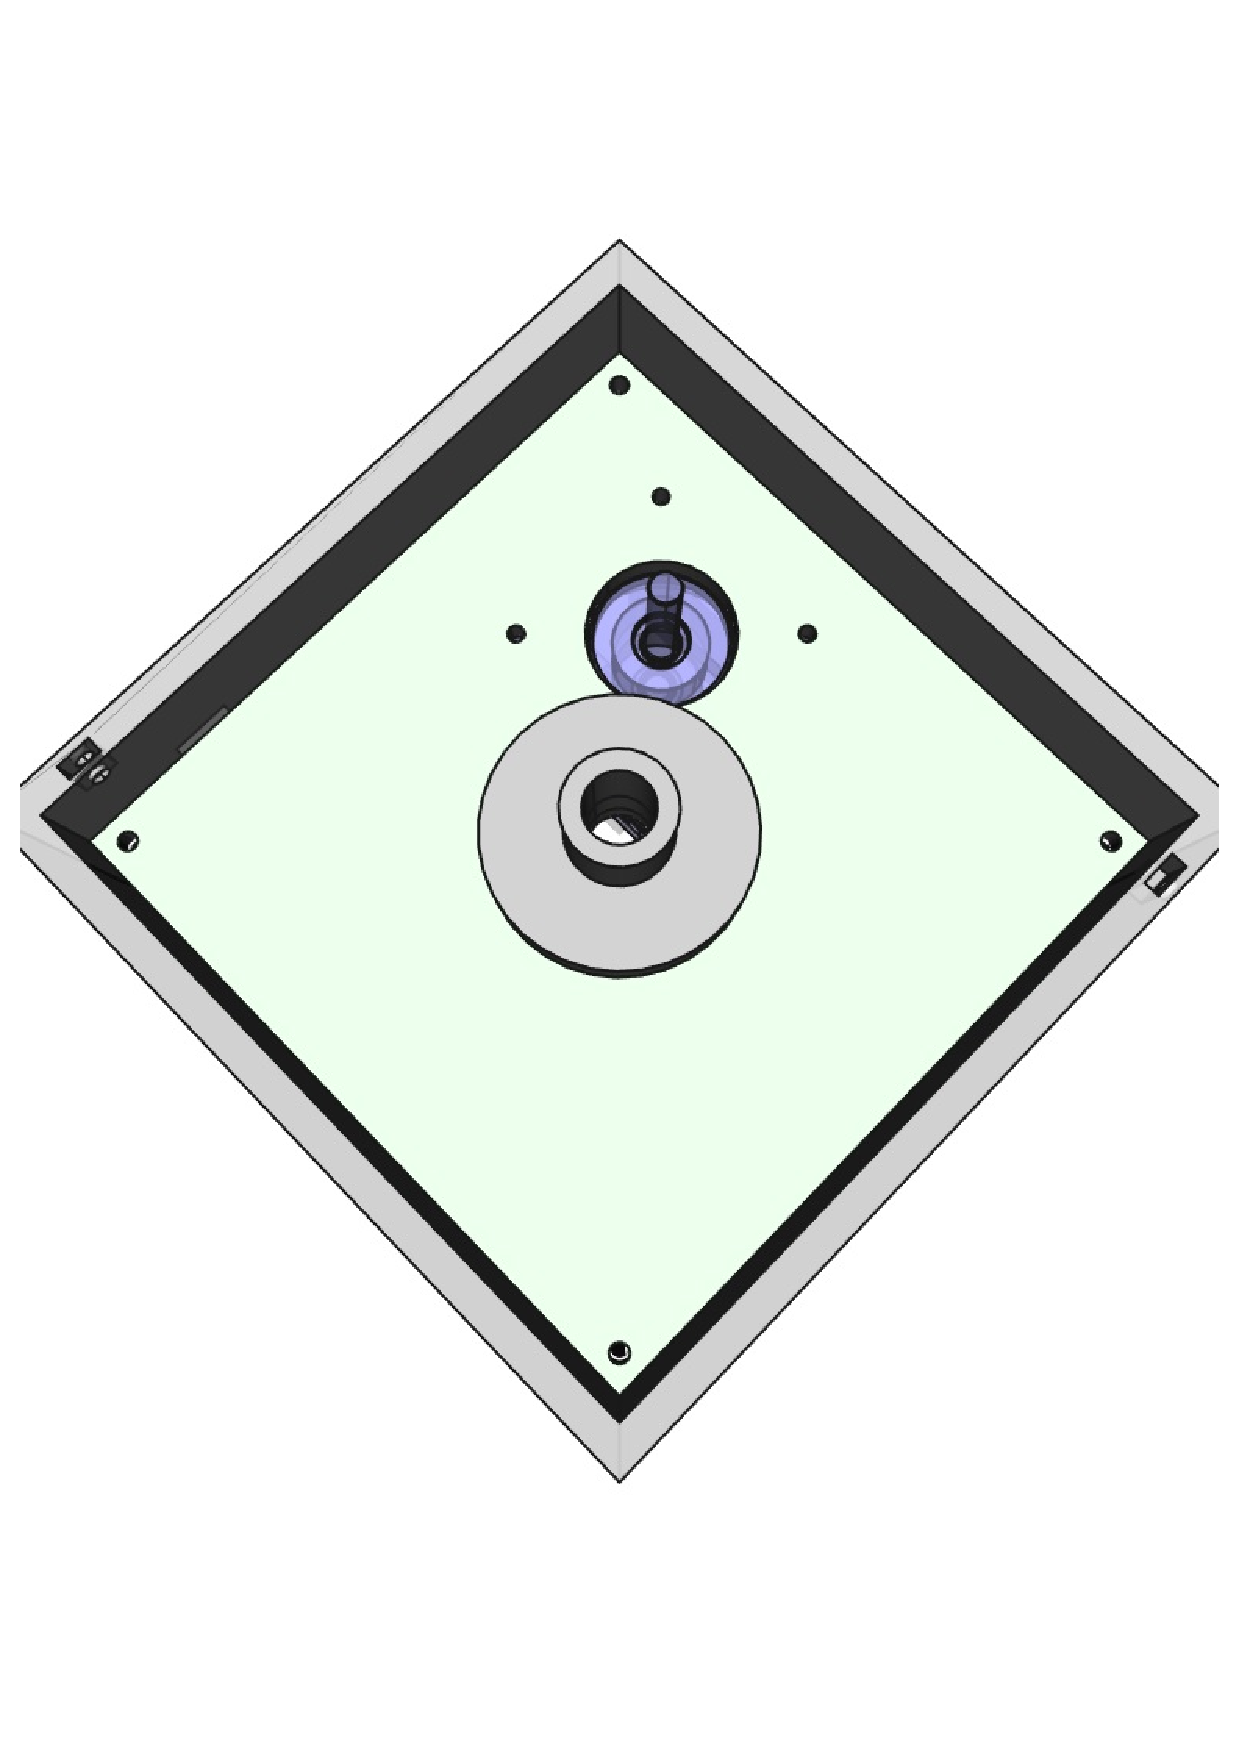
\includegraphics[trim= 0 100 0 100, clip, width=0.45\linewidth]{images/design/base/base_flat_surface.pdf}}
	\subfigure[base gear]
		{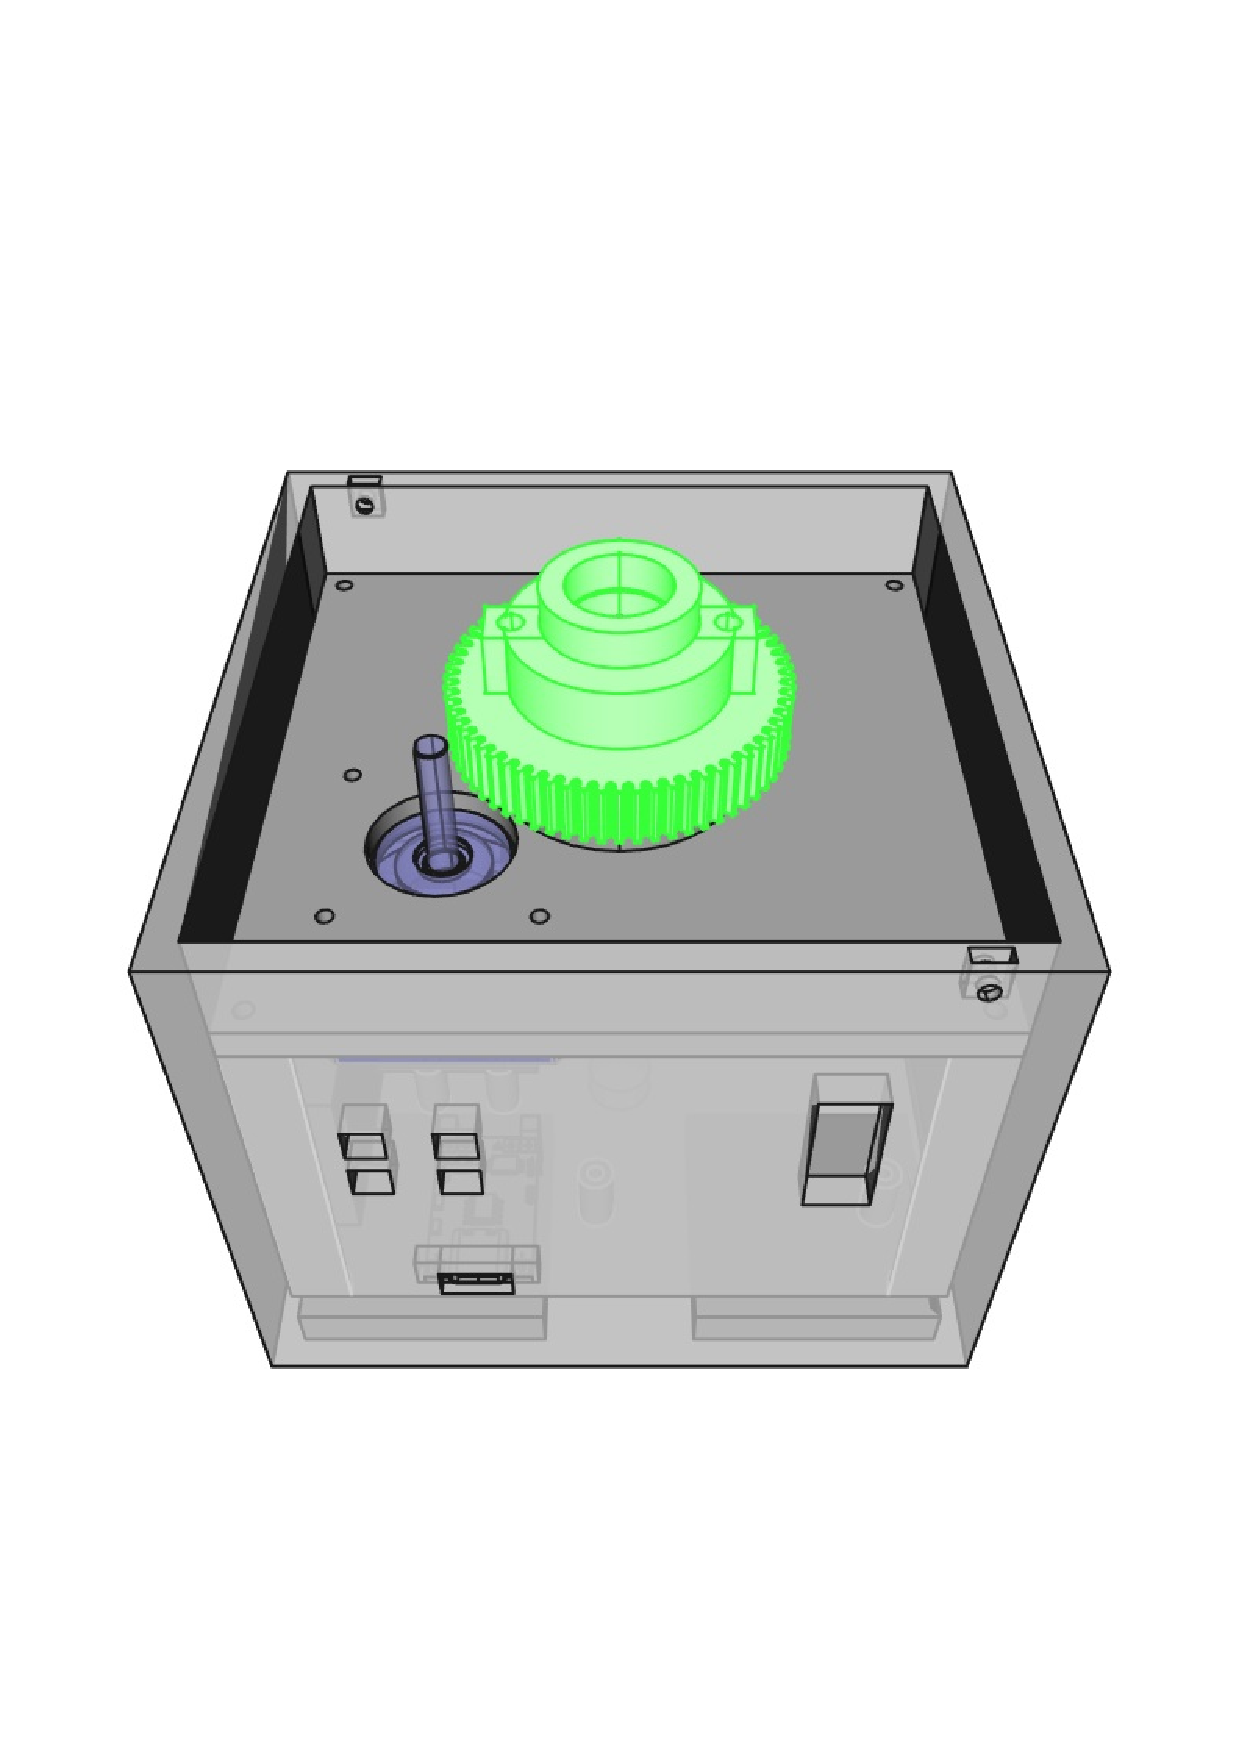
\includegraphics[trim= 0 100 0  200 , clip, width=0.45\linewidth]{images/design/base/base_gear.pdf}}
	\caption{In (a) is visible the flat surface that lies on top of the four columns, and in (b)the gear that rotates the \textit{middle} part.}
\end{figure}


The intermediate flat surface has also some holes to allow a motor to be mounted below it: on the motor, there is a \textbf{gear} that makes a bigger gear on the previously introduced cylinder to rotate; this in turns rotates the middle part. 
The bigger gear is also inserted on a bearing ball.


The lid simply keeps the bigger gear in place, and another bearing ball
where the middle part rests. It is screwed to the base with two screws on the side.

Another two holes were manually added on the side to allow the raspberry to be powered through the USB port, and to be connected with its Ethernet port. 

\subsection{Middle}

This part was not printed as one piece, but as three separate pieces: the bottom one and the two sides. The sides are screwed to the bottom part, to form a \textit{u} shape. 

\begin{figure}[H]
	\centering
	\inctrimpic[0.7]{images/design/middle/middle_iso.pdf}
	\caption{This is the \textit{middle} part of the star tracker, in green. The other parts are auxiliary parts mounted on it.}
	\label{fig:middle_iso}
\end{figure}

The middle part allows the system to rotate towards the north. On this part there is:

\begin{itemize}
	\item a \textbf{motor}, that moves \textbf{three gears}
	\item an \textbf{Adafruit} chip with magnetic, gyro and accelerometer sensors
\end{itemize}

The motor is mounted at the bottom, and is connected to three gears, to increase its output torque. This is essential because it can raise the \textit{top} part, according to the latitude read by the gps sensor. 

The two bigger gears have a cylinder in their middle, that is then inserted in bearing ball.

\begin{figure}[H]
	\centering
	\subfigure
		{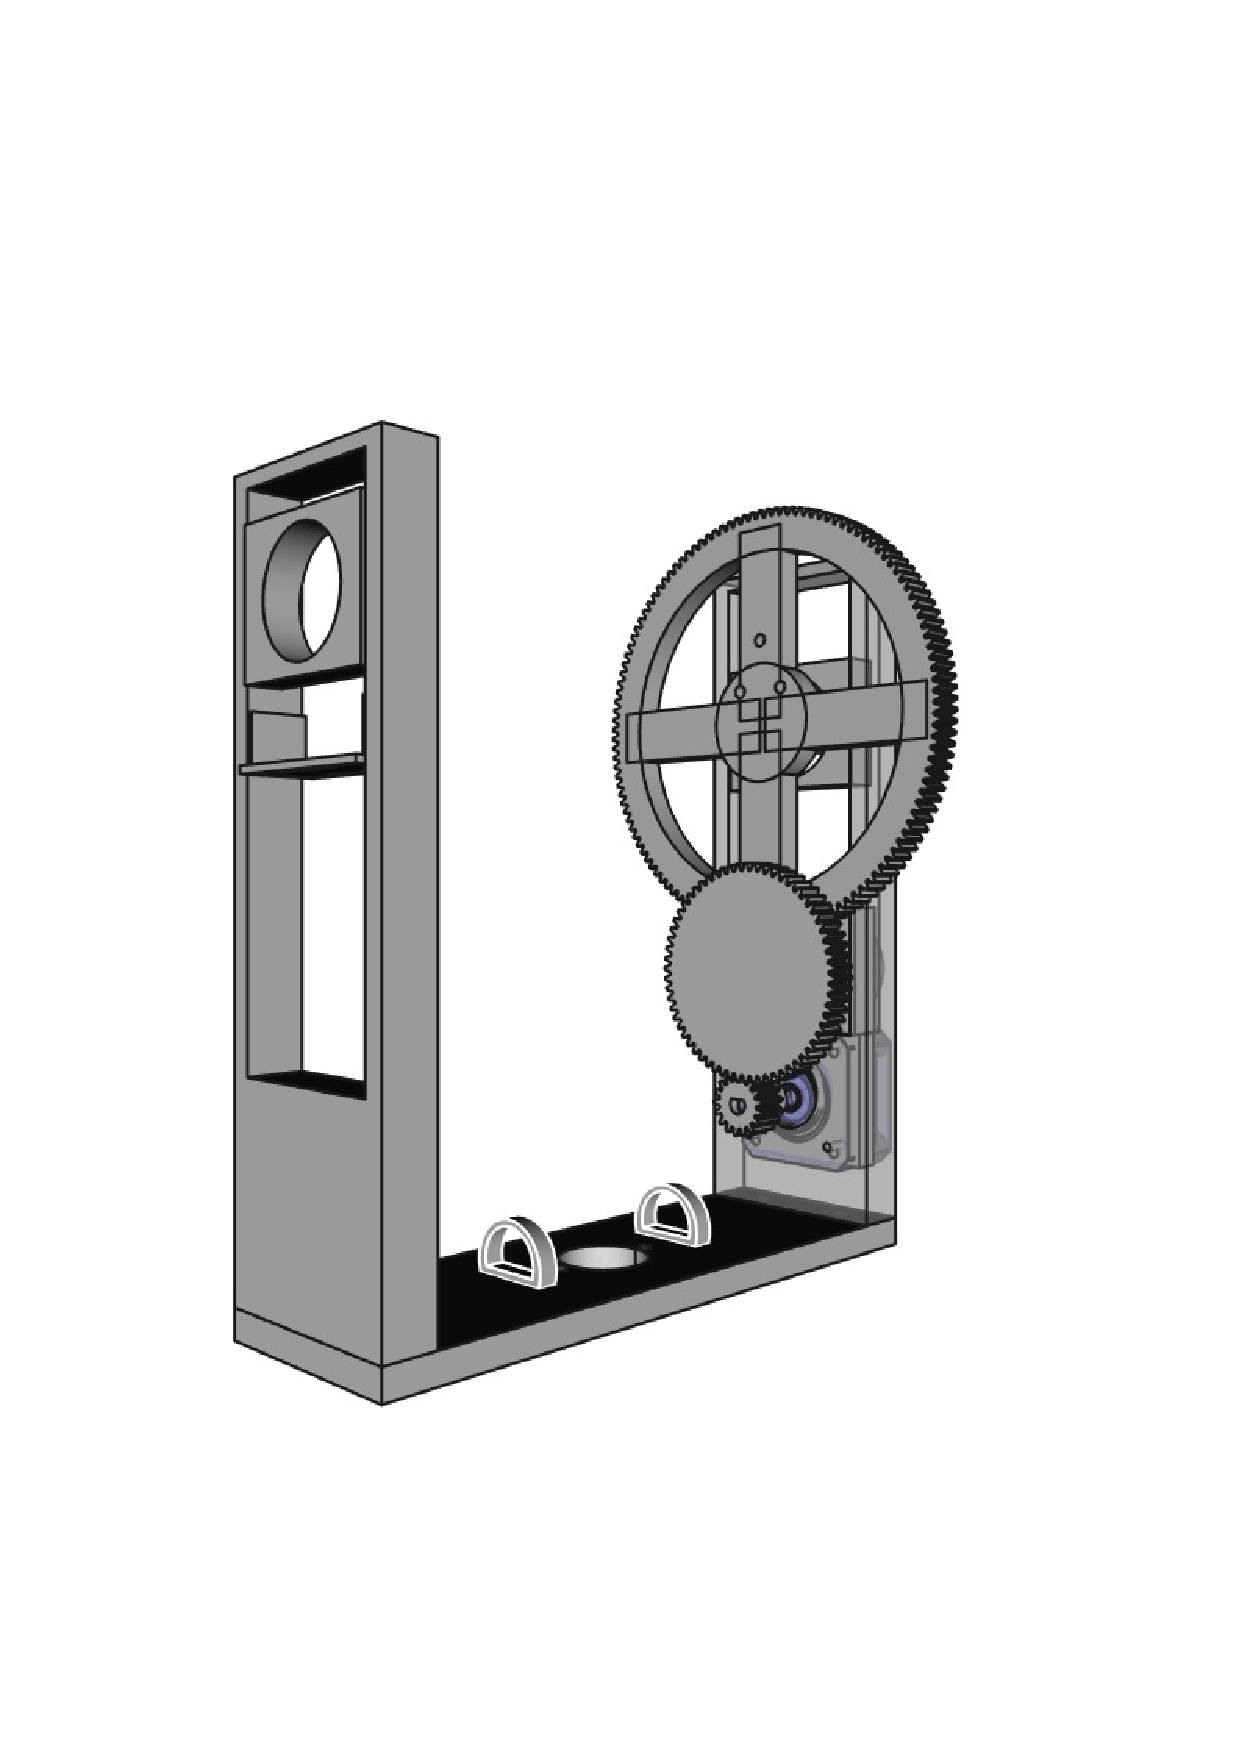
\includegraphics[width=0.45\linewidth]{images/design/middle/base_all}}
	\subfigure
		{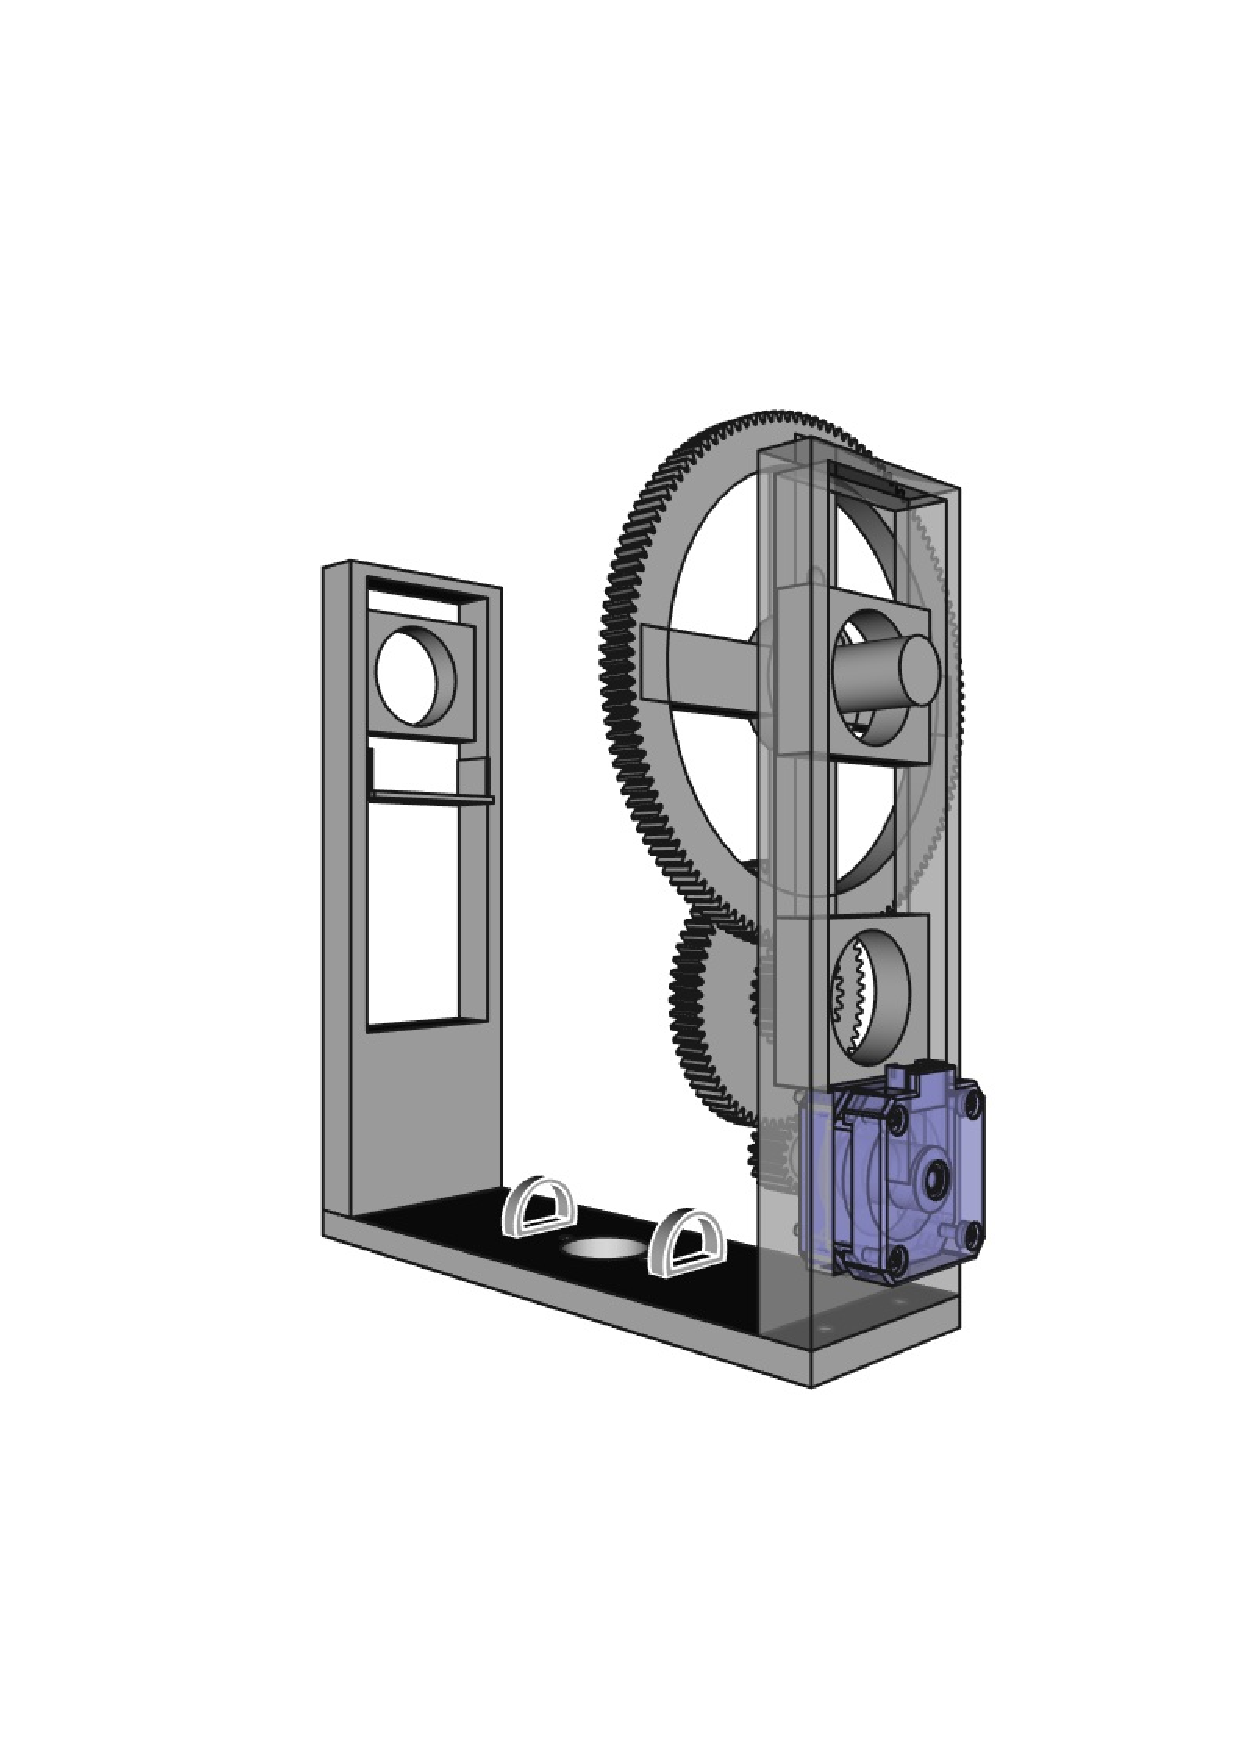
\includegraphics[width=0.45\linewidth]{images/design/middle/base_all2}}
	\caption{In this picture, all the other 3D printed parts are visible mounted on the \textit{middle} part. }
	\label{fig:middle_all}
\end{figure}

The bearing ball
is then fixed in another 3D printed rectangle, that is screwed on the sides of the "arms" of the \textit{middle} part. 
\\
\\
The Adafruit magnetometer sensor can be affected by the magnetic field generated by the motors, so it is mounted in the most far position possible on the opposite side of the motor. 

The \textit{top} part is supported thanks to some screws on the bigger gear on one side, and a bearing ball
on the other side. The bearing ball
is supported thanks to a 3D printed rectangle, as discussed before. 
\\
\\
At the bottom, the two small arcs are used to run the cables through them, to minimize the possibility of twisting. 

\subsection{Top}

The \textit{top} part is where the tracking actually occurs; here is mounted:
\begin{itemize}
	\item \textbf{3d printed parts} to attach it to the \textit{middle}
	\item a \textbf{motor} with two \textit{gears} and a \textbf{support} to attach a camera
	\item an \textbf{accelerometer sensor}
	\item a \textbf{motor driver}
	\item a \textbf{support} for a gear
\end{itemize}

This is also the simplest part: the accelerometer is used to determine the plane inclination. The inclination must be the same of the latitude. 

The gears provide the actual tracking: the camera is mounted on top of the biggest gear, that rotates accordingly to the rotation of the Earth, through  a support, that is actually screwed to the gear and connects them. 


\begin{table}[H]
	\centering
	\subfigure[]{\inctrimpic[0.32]{images/design/top/top_empty.pdf}}
	\subfigure[]{\inctrimpic[0.32]{images/design/top/top_sides.pdf}}
	\subfigure[]{\inctrimpic[0.32]{images/design/top/top_gear_support.pdf}}
	
	\subfigure[]{\inctrimpic[0.45]{images/design/top/top_gears.pdf}}
	\subfigure[]{\inctrimpic[0.45]{images/design/top/top_cam_support.pdf}}
	\caption{The \textit{top} part: (a) is empty; in (b), (c) and (d) 3D printed parts are
	 sequentially added. (e) shows the support where the camera can be screwed. }
	\label{tab:topseq}
\end{table}

\section{Motors and gears}

This section provides details about the motors and the gear moved by them. 

\subsection{Motors}
The motors were chosen with two main specifications:

\begin{enumerate}
	\item the motors should be \textbf{lightweight}, and requiring a small amount of \textbf{tension/current}
	\item the motors can be driven \textbf{precisely}
\end{enumerate}

Keeping the motors lightweight and with little electric requirements, allows for a more light overall structure, and to use a smaller battery, thus maintaining the star tracker more portable. 

On the other hand, if the weight that a motor needs to raise/move is too high, a well-crafted and thought \textbf{gear-set} must be used, introducing more complexity and requiring more space to insert it. The gears will be discussed in the next subsection.

As regards the second requirement, the most suitable type of motor to fulfil it is the \textbf{stepper motor}.

A stepper motor is an electromagnetic motor, that can be moved in \textbf{steps}, where each step corresponds to a certain degree of movement. A stepper motor can be driven in a way that each current impulse generates a certain amount of steps. 

For this project, two models of motor were chosen: a \textbf{Nema 17HS15}, to rotate the \textit{middle} part and incline the \textit{top} part, and a \textbf{Nema 17HS4023} for the tracking movement. These motors have the desired requirements, and are driven with two circuits that will be discussed in the next session. 

The motors' specification are summarized in table \ref{table:motor}.
\\
\\
The motor in the \textit{base} does not actually rotate the \textit{middle} part, but it \textbf{"vibrates"} (rotating very fast clockwise and anticlockwise) to tell the user how to rotate the part by hand; this solution was adopted because the 3D printed parts do not allow a precise installation and movement of them, and there is \textbf{too much friction} in some teeth of the gears to allow the motor to rotate them smoothly; so a "manually" approach was chosen, with the motor simply used to act as an indication for the user, who performs the action in place of the motor. 

Other than movement/vibration, the motors perform another important function: they lock the gears in place, to stop them from moving after being placed in the right position.

\begin{table}
	\centering
	\begin{tabular}{|c|c|c|c|c|}
		\hline
		Name & Stepping Angle & Current & Tension & Torque \\
		\hline
		\textbf{Nema 17HS15} & $1.8^\circ$ & $1.5A$ & $12V$ & $45N\cdot cm$ \\
		\hline
		\textbf{Nema 174023} & $1.8^\circ$ & $1A$ & $4V$ & $13N\cdot cm$ \\
		\hline
	\end{tabular}
	\caption{Motors' specifications.}
	\label{table:motor}
\end{table}

\begin{figure}[h]
	\centering
	\inctrimpic[0.7]{images/motors/motors_placement}
	\caption{Motors' placement: the purple one is a different model than the red ones.}
	\label{fig:motorplacement}
\end{figure}


\subsection{Gears}
In this subsection, the design of the gears is discussed; after introducing the gears individually, they are presented as gear-sets. The table \ref{tab:gears}
summarizes all the gears used. 
\begin{table}
	\centering
	\begin{tabular}{|c|c|c|c|}
		\hline
		N. of teeth & Module & Positions & N. of gears \\
		\hline
		17 & 0.8 mm & \textit{base, top\tablefootnote{The gear in the top is a helicoidal gear, although with the same specifications.}} & 2 \\
		\hline
		64 & 0.8 mm & \textit{base} & 1 \\
		\hline
		17 & 1 mm & \textit{middle} & 1 \\
		\hline
		24, 64\tablefootnote{
		This gear is composed of two gears printed one on the other. 
		} & 1 mm & \textit{middle} & 1 \\
		\hline
		127 & 1 mm & \textit{middle} & 1 \\
		\hline
		126 & 0.8 mm & \textit{top} & 1 \\
		\hline
	\end{tabular}
	\caption{Table representing all the gears used; the last column refers to the number of printed gears.}
	\label{tab:gears}
\end{table}


The gears were designed with the CAD software \textit{Freecad}, using the \textit{part design} mode. 

A gear can be simply created specifying the \textbf{number of teeth} and the \textbf{module}, which is the number of millimeters of pitch diameter divided by the number of teeth and is used to describe the size of the teeth.

\subsubsection{Base gears}

There are only two gears: one, which is screwed to the motor, and the other, which is connected to the first and provides the rotation to the \textit{middle} part.

The first gear has 17 teeth, the second 64. The first gear has a "hole" on its side, so a nut can be inserted to screw in a bolt which pressed against the motor shaft to keep it in place.

The 64 teeth gear has an empty space at its bottom to contain a bearing ball.

\begin{figure}[h]
	\centering
	\subfigure{\inctrimpic[0.45]{images/motors/mot_17_mod08.pdf}}
	\subfigure{\inctrimpic[0.45]{images/motors/mot_17_mod08_2.pdf}}
	\caption{The 17 teeth gear in the \textit{base}.}
	\label{fig:17base}
\end{figure}

\begin{figure}[h]
	\centering
	\subfigure{\inctrimpic[0.45]{images/motors/mot_64_mod08.pdf}}
	\subfigure{\inctrimpic[0.45]{images/motors/mot_64_mod08_2.pdf}}
	\caption{The 64 teeth gear in the \textit{base}. In the second image, the space for the bearing ball is visible.}
	\label{fig:64base}
\end{figure}

It is now possible to consider the gears as a \textbf{gear-set} and compute the \textbf{output torque}. 

The formula to compute it, which will be also used in the next subsections, is the following:

$$ \textnormal{output torque} = \frac{\textnormal{teeth of driven}}{\textnormal{teeth of driver}}\cdot \textnormal{input torque}$$
\\
\\
The motor used in the \textit{base} produces around \textbf{17} $N\cdot cm$ of \textbf{torque}. Since this output is applied to a 17 teeth gear, which is connected to a 64 teeth, this gives an output of around $ \frac{64}{17}\cdot{17} = 64 N\cdot cm$.

In the actual setup, the motor is rated for 1 Ampere of current, the driver nominal continuous current is $0.8A$, with peaks above $1A$; since the torque depends is proportional on the current \cite{steppermcurrent}, the output torque should be lower. 

In fact, this motor is used as a "vibrator", and not to move the upper parts, as will be described in section \ref{sec:software}, in the paragraph dedicated to the gps and north alignment. The user itself rotates the \textit{middle} part, using the indications provided by the motor's vibration.

\subsubsection{Middle gears}

In the \textit{middle} part, there are 4 gears, although 2 of them are printed together. 

The smallest one, is identical to the one in figure \ref{fig:17base}, except for the module, which is slightly larger. 

In this setup, there are more gears connected, but the formula to compute the output torque is the same. The second gear consists of a 24 teeth and a 64 teeth gears, and has a cylinder to be put inside a bearing ball, and facilitate its rotation. Its function is to connect the 17 teeth to the 127 teeth gear, which is also connected to a bearing ball.

\begin{figure}[h]
	\centering
	\subfigure[]{\inctrimpic[0.45]{images/motors/mot_middle_64_24.pdf}}
	\subfigure[]{\inctrimpic[0.45]{images/motors/mot_middle_127.pdf}
	}		
	
	\subfigure[]{\inctrimpic[0.7]{images/motors/mot_middle.pdf}}
	\caption{(a) is the 24/64 teeth gear, (b) is the 127 teeth gear and (c) are all the gears connected with the motor.}
	\label{fig:middle_gears}
\end{figure}


The purpose of the 127 teeth gear is to rotate the \textit{top} part.

These gears are connected to another $17 N \cdot cm$ motor; so the output torque $OT$ is given from:



\begin{align*}
	OT & = \frac{64}{17}\cdot \frac{127}{24}\cdot 17 \\
	   & = 3.76 \cdot 5.29 \cdot 17\\
	   & = 338.14 N\cdot cm
\end{align*}
\newpage
\subsubsection{Top gears}


There are two \textit{top} gears, a smaller one connected to the motor, and a bigger one, which rotates the camera and provides the actual tracking (fig. \ref{fig:topgears}). These gears differ from the others because they are double helicoidal, to provide better contact between them. 

These gears have 17 and 126 teeth; they are connected to a more powerful motor than the other gears; the torque of the motor is:

\begin{align*}
	OT & = \frac{126}{17}\cdot 45 \\
	& = 333.53 N\cdot cm
\end{align*}

\begin{figure}[H]
	\centering
%	\subfigure[]{\fbox{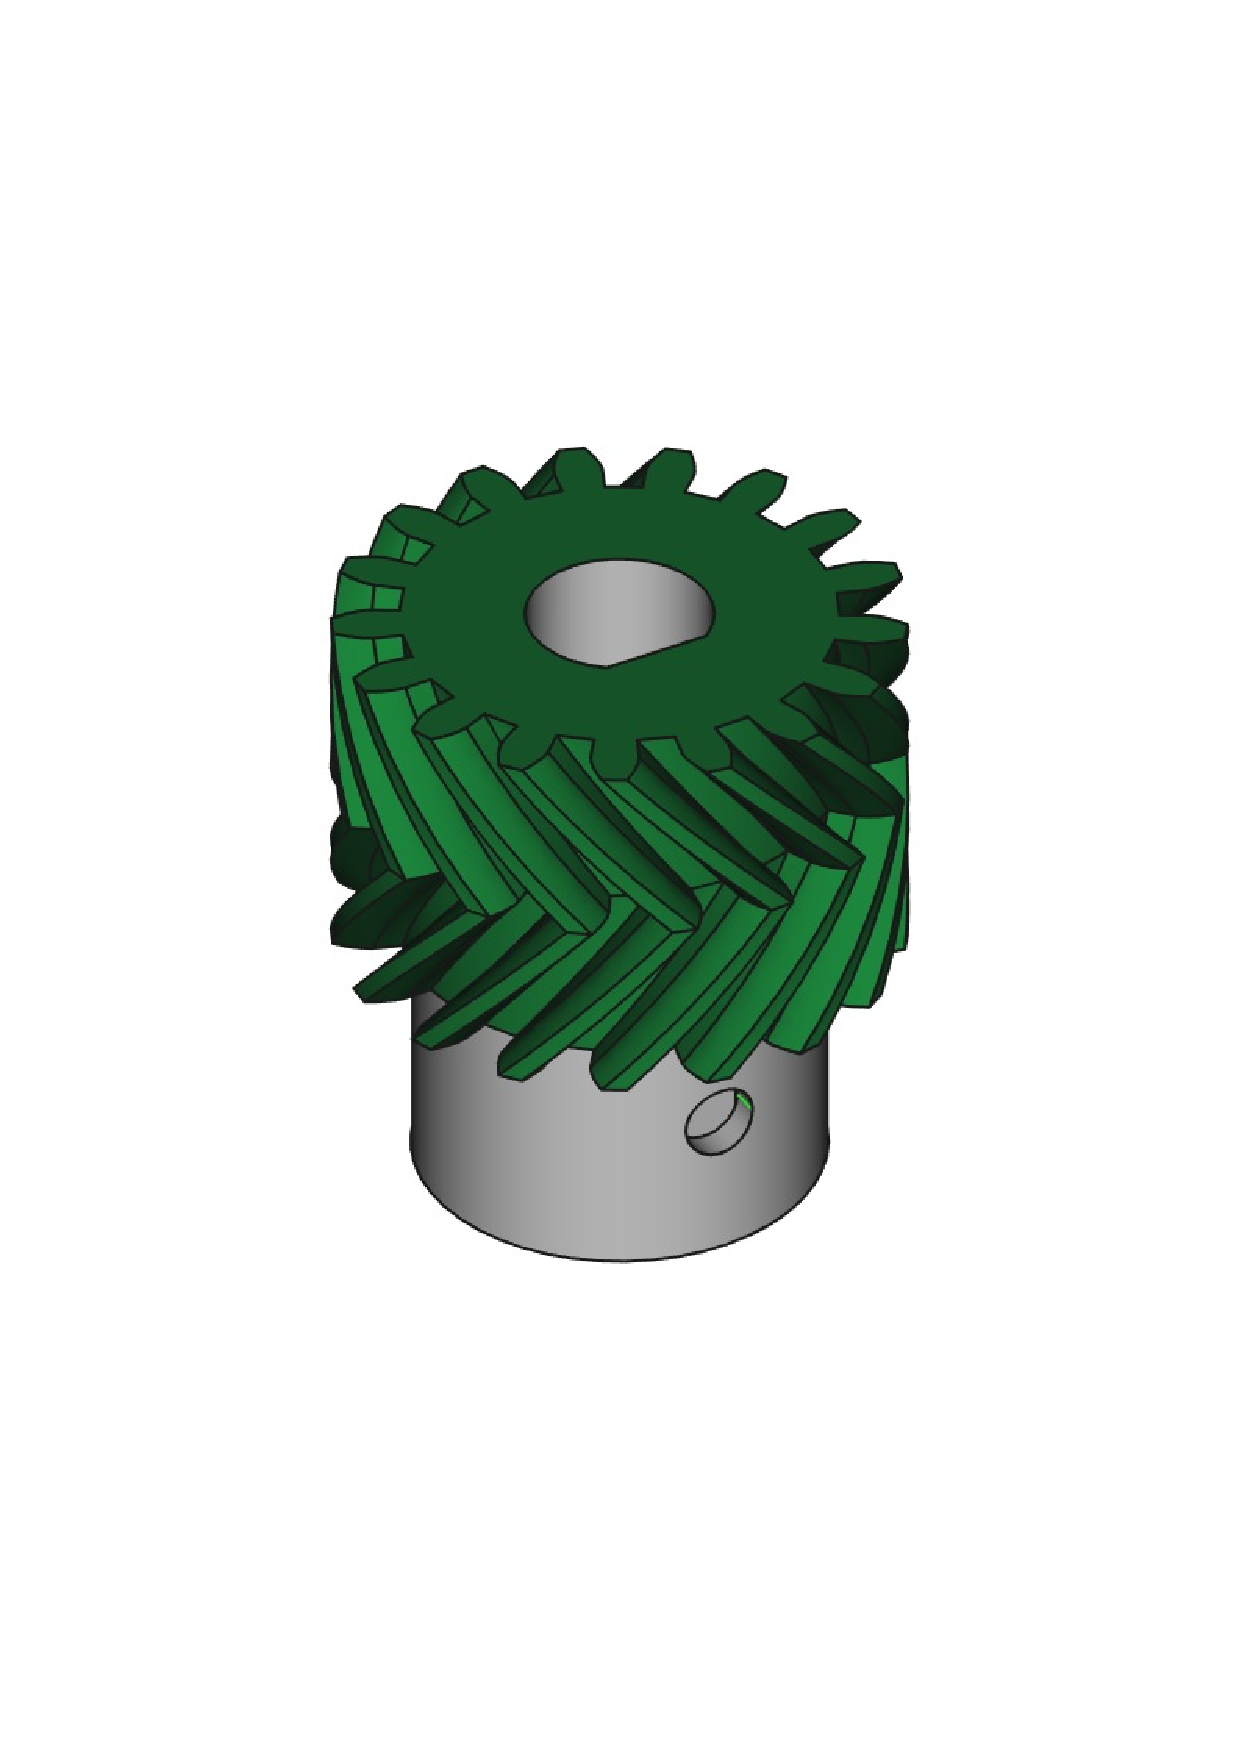
\includegraphics[trim=0 200 0 200, clip, width=0.45\linewidth]{images/motors/mot_top_gear_17.pdf}\label{fig:topgears1}}}
	\subfigure[]{\inctrimpic[0.45]{images/motors/mot_top_gear_17.pdf}\label{fig:topgears1}}
	\subfigure[]{
		\inctrimpic[0.45]{images/motors/mot_top_gear_126.pdf}\label{fig:topgears2}
		}
	\subfigure[]{\inctrimpic[0.6]{images/motors/mot_top_gears.pdf}\label{fig:topgears3}}
	\caption{(a) is the small, 17 teeth \textit{top} gear; (b) is the bigger, 126 teeth \textit{top} gear; (c) shows the disposition of the two gears together. In (a) the double helicoidal pattern of the teeth is very noticeable.}
	\label{fig:topgears}
\end{figure}

The camera does not sit directly on top of the 126 teeth gear; there is a support (it is cyan in figure \ref{fig:topgears3}).

The support allows for a camera ball-head to be mount on it, such as the one in figure \ref{fig:camerahead}, with a screw holding them together.


\begin{figure}[h]
	\centering
	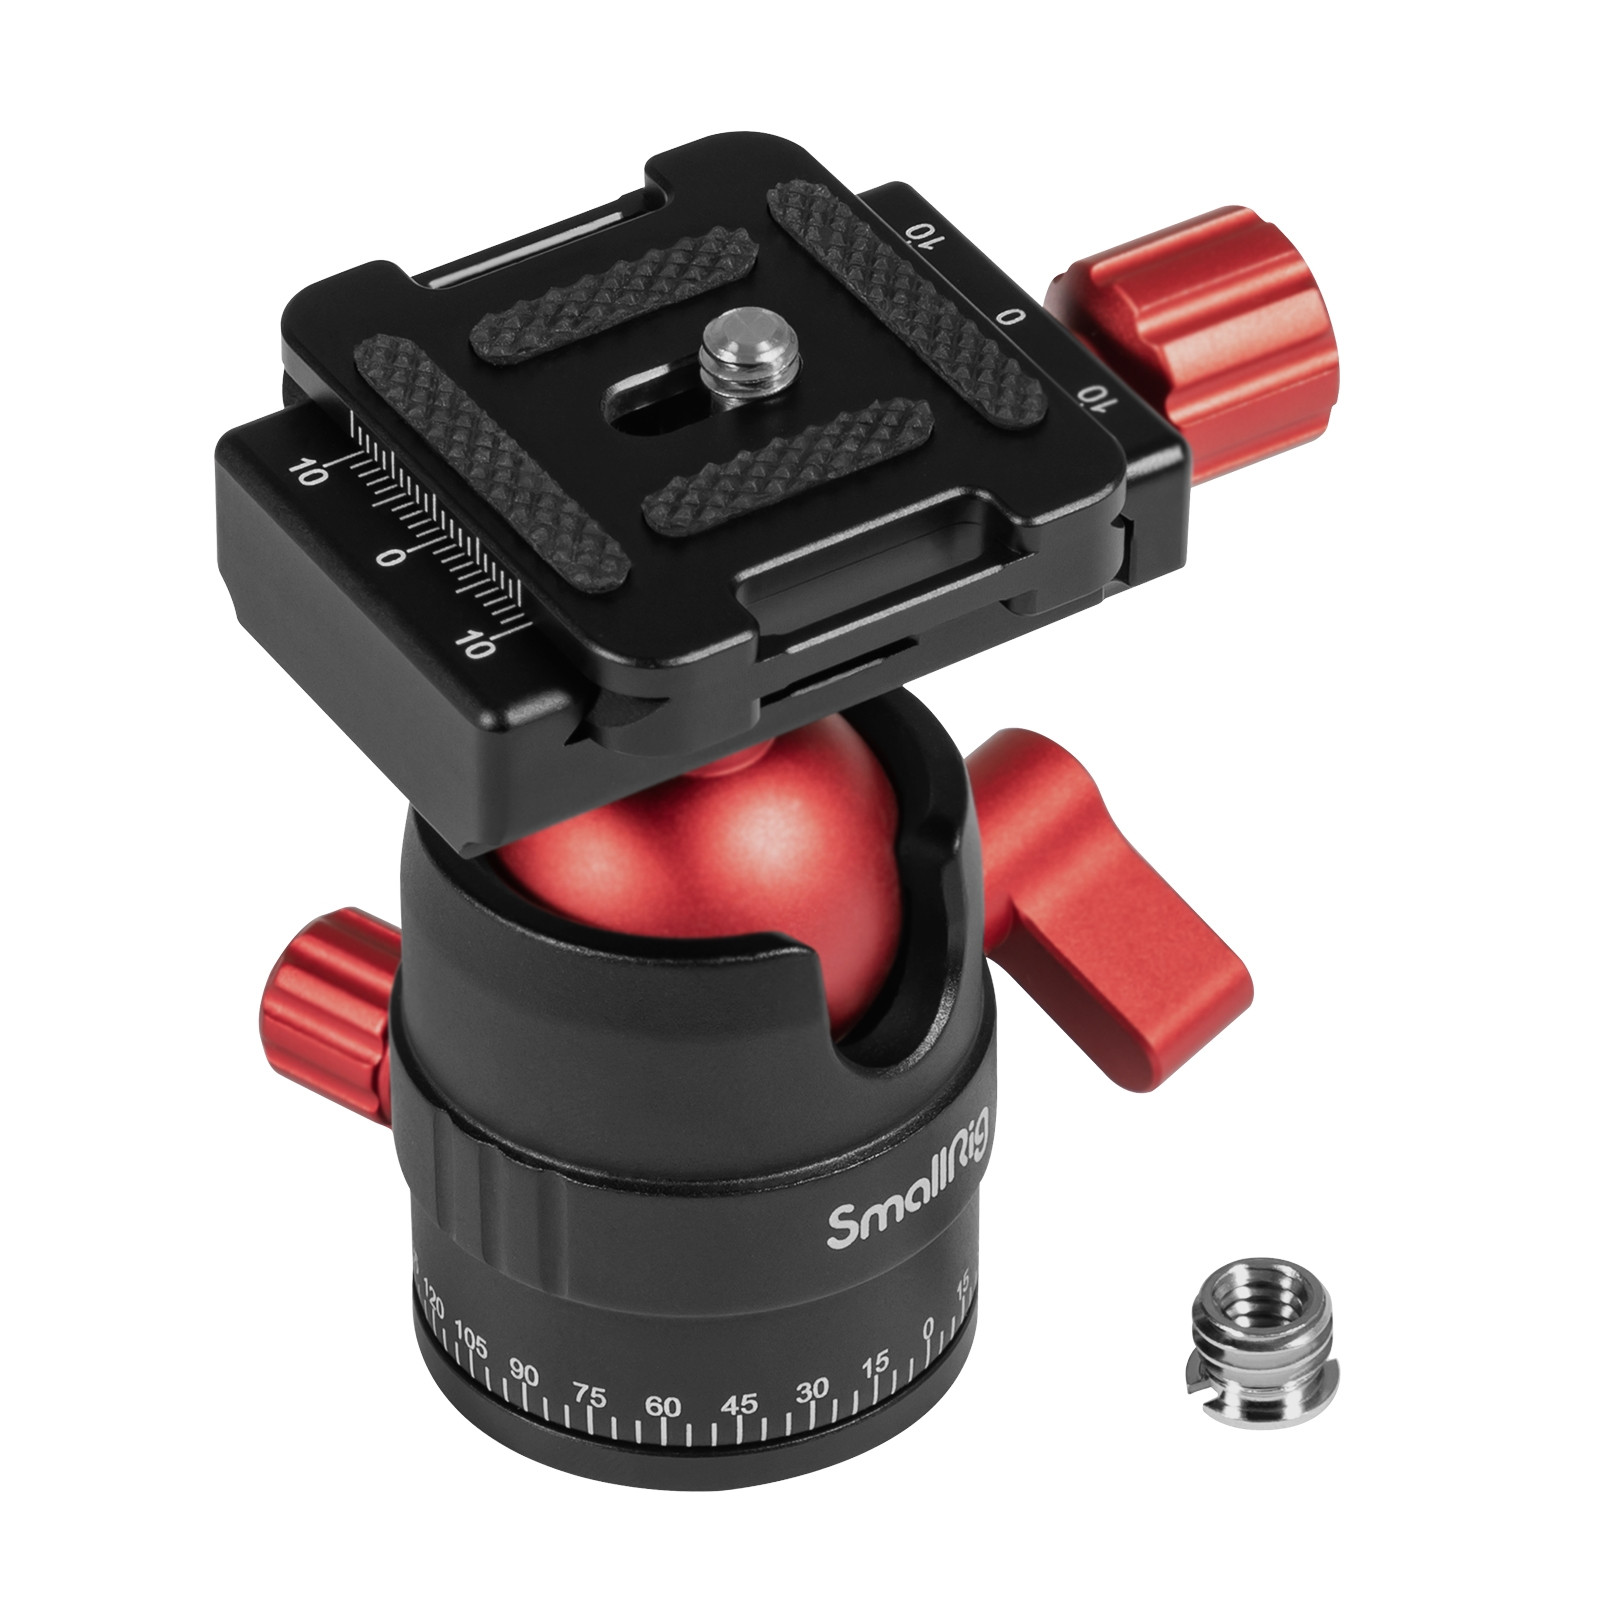
\includegraphics[width=3.5cm]{images/motors/camballhead.jpg}
	\caption{A camera ball-head that can be mounted on the support on the 126 \textit{top} gear.}
	\label{fig:camerahead}

\end{figure}

Since the camera is placed on the \textit{top} plane, which can be tilted by some degree $\alpha$ (figure \ref{fig:moment}) with reference to the ground, it is possible to compute whether the motor can turn the camera for various values of $\alpha$. For simplicity, only rotation in the $xz$ plane will be considered (figure \ref{fig:xzplane}). 

\begin{figure}[H]
	\centering
	\subfigure[]{
		\begin{tikzpicture}
			\pgftext
			[at=\pgfpoint{0cm}{0cm},left,base]
			{
				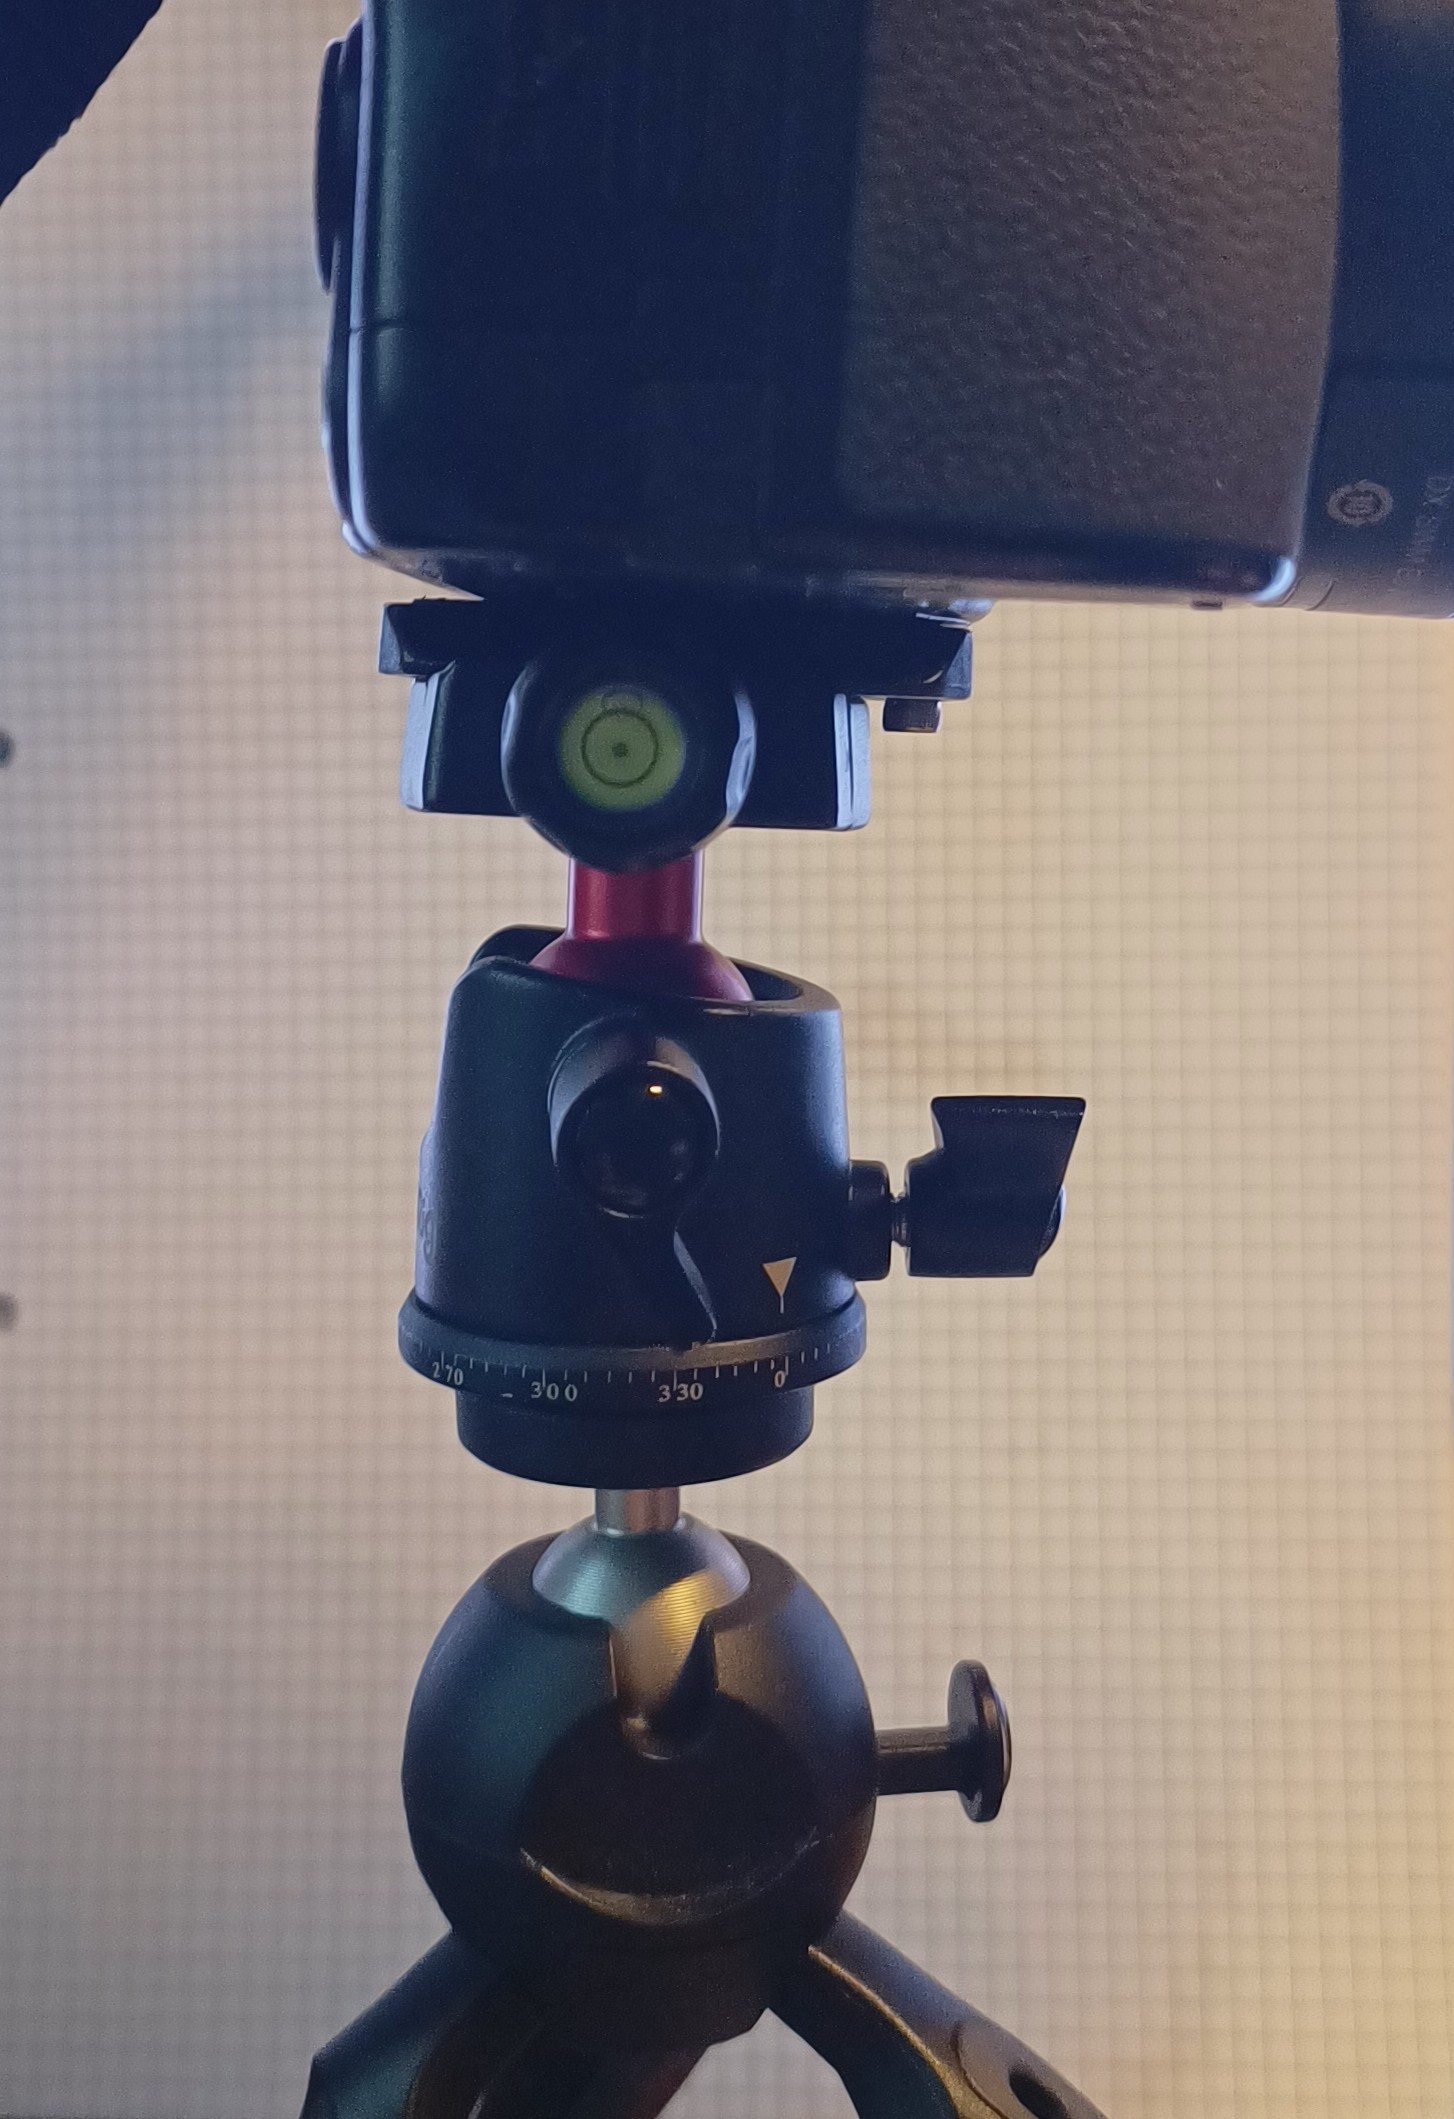
\includegraphics[ height=5.5cm]{images/motors/cm_photo1.jpg}
			}
			\node (orig) at (0.5, 1.2) [draw=none] {};
			\draw[line width=1pt, color=white, arrows=->] (orig) -- +(0, 2);
			\draw[line width=1pt, color=white, arrows=->] (orig) -- +(2, 0);
			
			\node (xt) at ($(orig) + (0, 2.1)$) [draw=none, color=white] {z};
			\node (xt) at ($(orig) + (2.1, 0)$) [draw=none, color=white] {x};
		\end{tikzpicture}
		\label{fig:xzplane}
	}
	\subfigure[]{
		\begin{tikzpicture}
			\pgftext
			[at=\pgfpoint{0cm}{0cm},right,base]
			{
				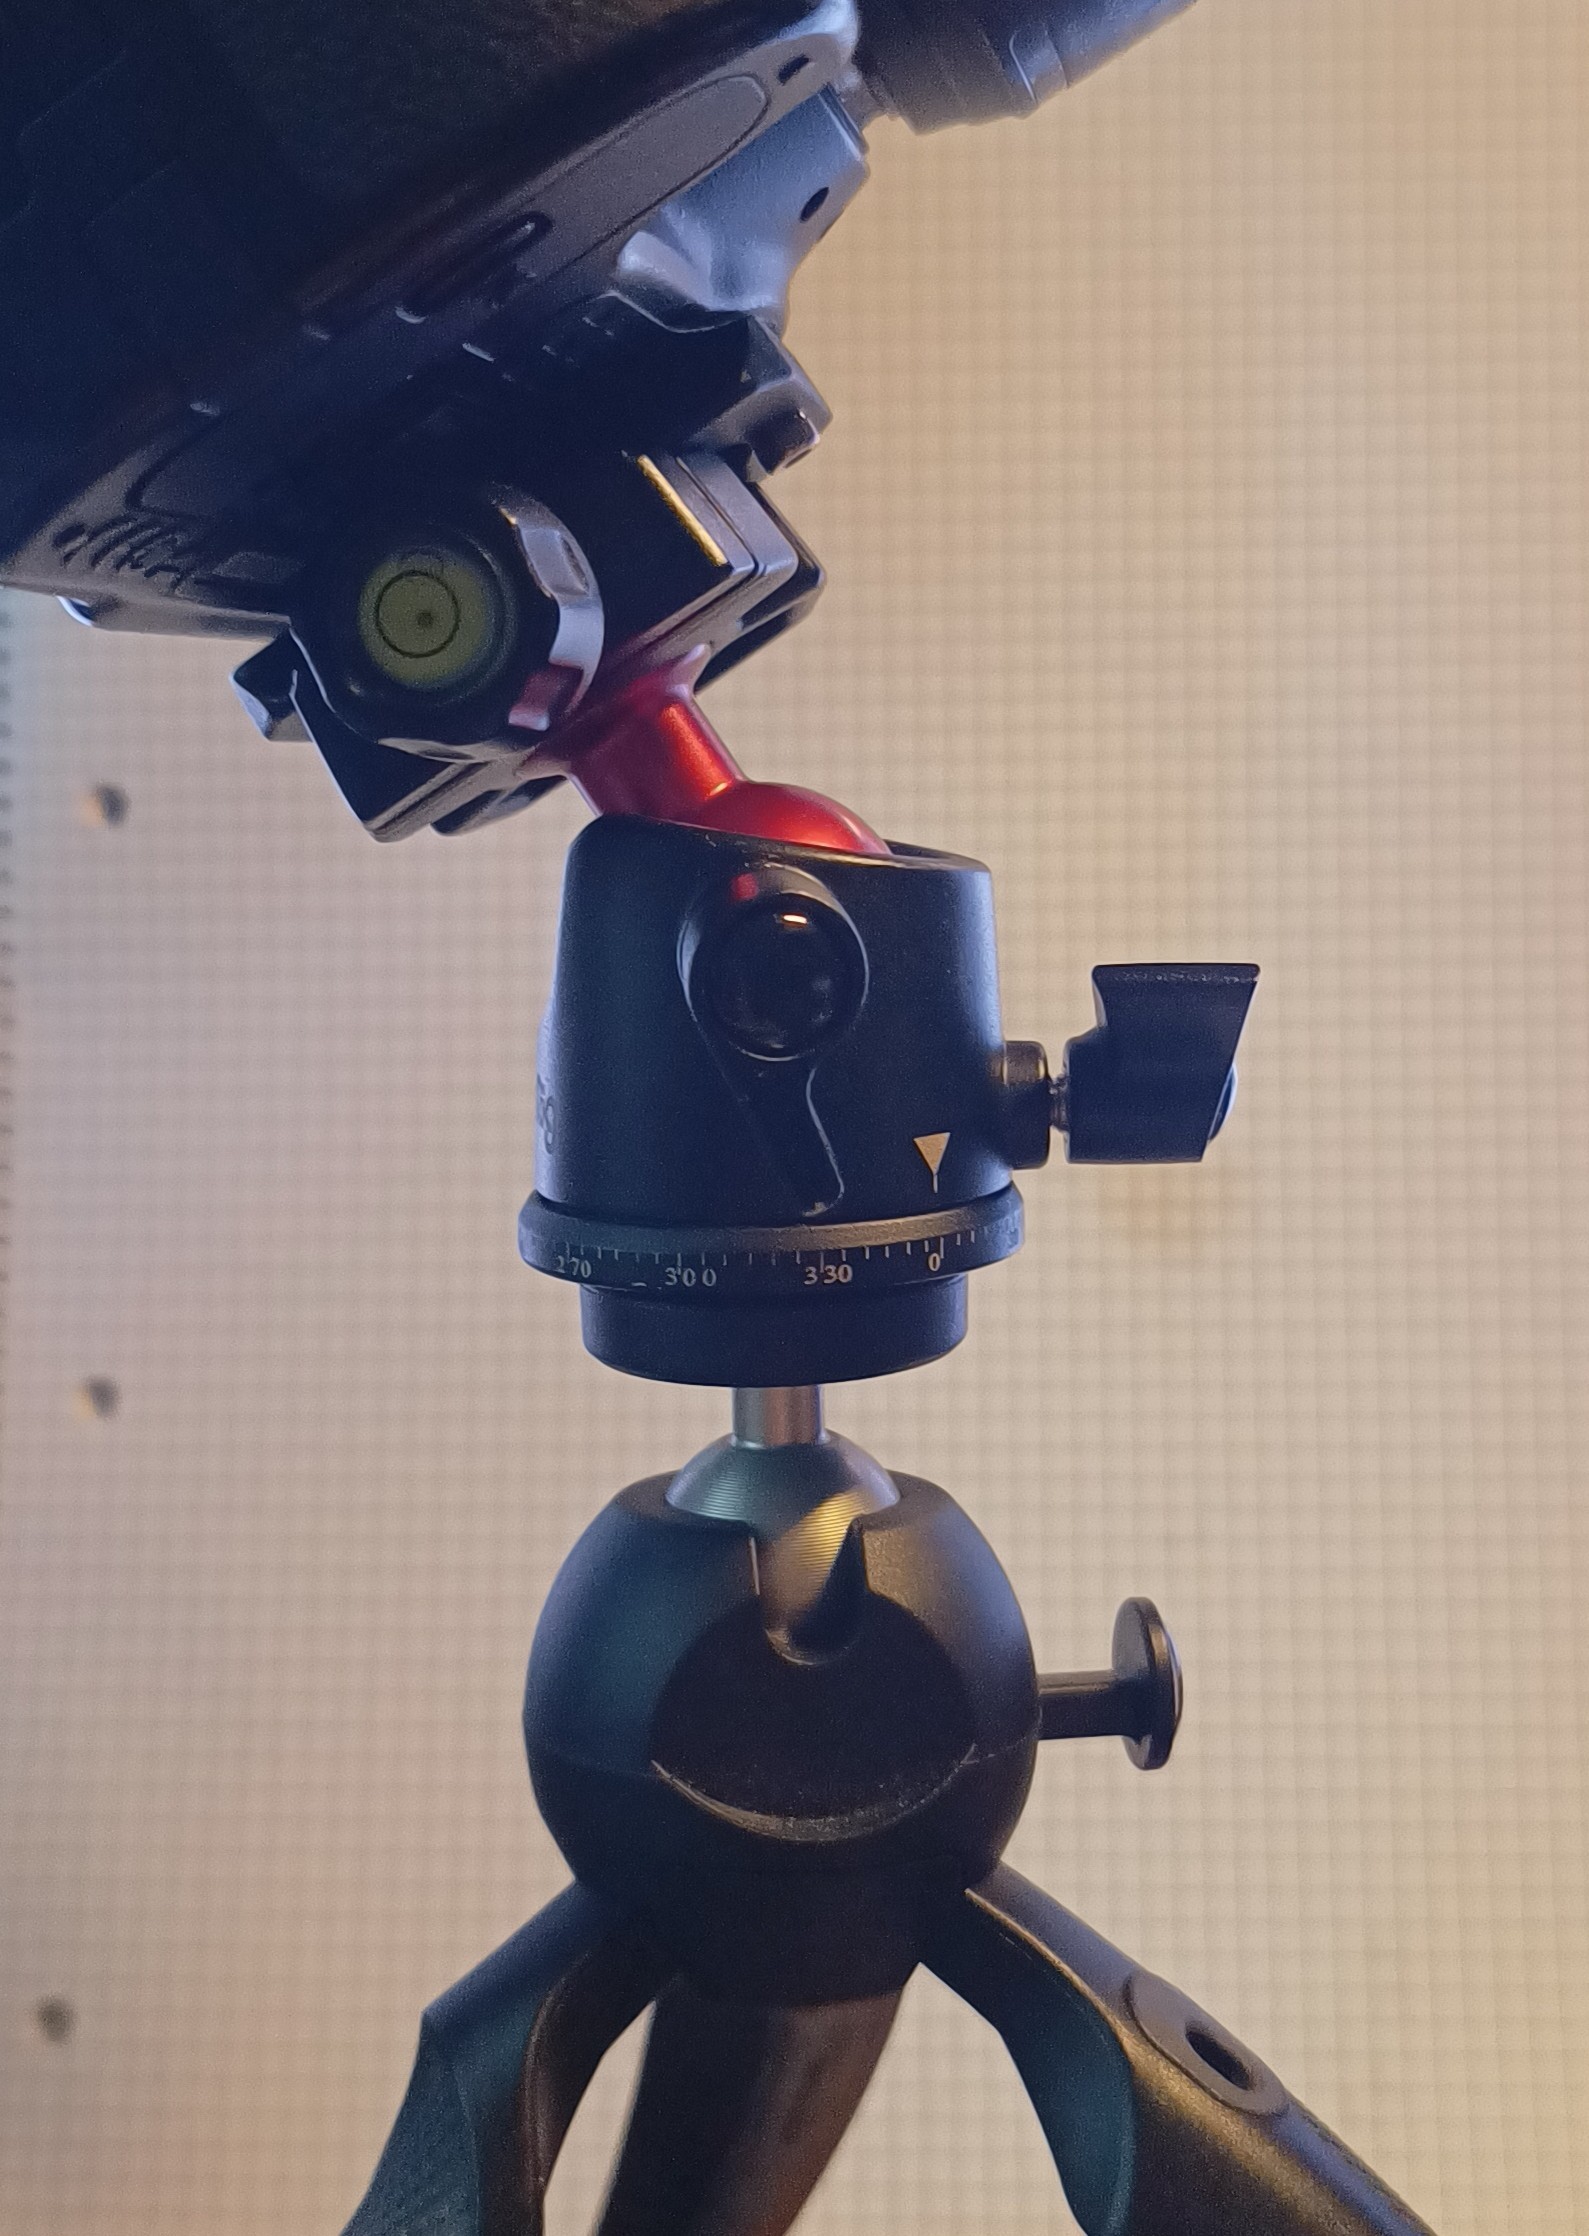
\includegraphics[ height=5.5cm]{images/motors/cm_photo2.jpg}
			}	
			\node (base) at (-2, 2) [inner sep=1pt, circle, fill=orange] {};
			\draw [line width=2pt, color=white] 
			(base)+(-1, 0) -- +(1, 0) ;
			\fill[pattern = north east lines, pattern color=white]  ($ (base) + (-1, 0) $)  rectangle  ($ (base) + (1, -.2) $)  ;
			
			\node (G) at ($(base) + (-0.1, 1.4)$) [circle,draw=white,inner sep=1pt,fill=red] {};
			\draw[line width=.6pt, color=black] (G)+(-1, 0) -- +(1, 0) ; 
			\draw[line width=.6pt, color=blue] (G)+(-1.1, -0.1) -- +(.9, 1.3) ; 
			\draw[thick, color=orange] (G)+(.5, 0) arc (0:45:1.1cm);
			
			\node (groundt) at ($(base) + (0, .2)$) [draw=none, scale=0.7, white] {ground};
			\node (betat) at ($(G) + (.3, .3)$) [draw=none, color=orange, scale=.7] {$\beta$};
			\node (betat) at ($(G) + (1, .15)$) [draw=none, color=black, scale=.5] {\textit{top} plane};
		\end{tikzpicture}	
		\label{fig:beta}
	}
	\caption{(a): only rotation in $xz$ plane will be considered; the camera is also parallel to the \textit{top} plane, i.e. the head-ball is not rotated. Note that, in general, the \textit{top} plane can be at various angles $\alpha$ w.r.t the ground. (b): $\beta$ is the angle of the camera w.r.t. the \textit{top} plane.}
\end{figure}


\begin{figure}[H]
	\centering
	\begin{tikzpicture}		
		\pgftext[at=\pgfpoint{0cm}{0cm},left,base]
		{\inctrimpic[1]{images/motors/cm_render_45_3.pdf}};
		% ...
		
		\node (base) at (9, 0) [draw=none] {};
		\draw [line width=2pt, color=black] 
		(base)+(-6, 0) -- +(2, 0) ;
		\fill[pattern = north east lines]  ($ (base) + (-6, 0) $)  rectangle  ($ (base) + (2, -.5) $)  ;
		\draw[thick, color=orange] (base)+(-1,0) arc (180:140:1cm);
		\node at ($ (base) + (-1.1, 0.4) $) [draw=none] {\color{orange}$\alpha$};
		
		\node (G) at (5.2,3.7)
		[circle,draw=black,inner sep=2pt,fill=red]
		{};
		%		\draw[gray,dashed, thick,line width=1pt] (G) circle (2.3cm);
		
		
		\draw[line width=2pt,shorten <=6pt, color=blue]
		(G)+(4,-4) -- +(-4,4)
		node[draw=none,inner sep=0pt,fill=none] (V1)
		{};
		%		\node (X) at (7.1, 4.2)
		%		[draw=none]
		%		{};
		\draw[line width=2pt,arrows=->, color=red]
		(G) -- +(.3,2.8)
		node[below, inner sep=2pt,fill=black, circle] (CM)
		{};
		\node at (CM) [draw=none, above=0.2cm] {Centre of mass};
		
		%		\draw[line width=1.5pt, arrows=<->, color=green]
		%		(CM)+(0.1, 0.1) -- +(-2, -1.5) node[draw=none] (D) {}; %distance from axis of rotation
		\draw[line width=2pt, arrows=->, color=black]
		(CM) -- +(0, -3.5) node[draw=none, below] (F) {$F$}; %weight force
		\draw[line width=1.5pt, dashed, color=gray]
		(F) -- +(-2,2) node[draw=none] (vFh) {}; %vertical force helper
		\draw[line width=1.5pt, dashed, color=gray]
		(F) -- +(2,2) node[draw=none] (hFh) {}; %horizontal force helper
		\draw[line width=1.5pt, arrows=->, color={rgb:red,4;green,2;yellow,1}]
		(CM) -- +(1.8, -1.8) node[draw=none] (hF) {}; %horizontal component of the force
		\draw[line width=1.5pt, arrows=->, color=purple]
		(CM) -- +(-1.8, -1.8) node[draw=none] (vF) {}; %vertical component of the force
		
		
		
		\path (G)
		to node [below left=.2cm]
		{Axis of rotation} (G);
		\path (vF)
		to node [left]
		{$F_{\parallel}$} (vF);
		\path (hF)
		to node [below right=0.1cm]
		{$F_{\perp}$} (hF);
		%		\path (X)
		%		to node [left=0.2cm]
		%		{Lever arm} (CM);
		
		
		\draw[line width=2pt, color=red, arrows=->]
		(7.8, 2.7) -- +(1.5, 1.5) node[draw=none, left] (T) {\color{black}$T$};
	\end{tikzpicture}
	\caption{$\alpha$ is the angle between the \textit{top} plane and the ground. The weight force can be decomposed in a parallel and a perpendicular components, due to the angle of inclination $\alpha$. This force tries to rotate the gear, inducing a moment. The motor opposes this rotation, exercising a force $T$. }
	\label{fig:moment}
\end{figure}

To begin with, let's compute the \textbf{position of the centre of mass } of the camera. The dimensions that will be used are of the model Nikon D3300, the same used also for the tests. Its camera body can be roughly approximated with a parallelepiped, while the lens can be approximated with a cylinder. The body measures $124 \times 98 \times 76 mm$, while the the lens measures $73mm $ for the diameter and $79.5 mm$ in length.

The camera is mounted on top of a ball-head that can rotate in any direction, and form an angle $\beta$ with reference to the \textit{top} plane, but for now we will consider only the case where the camera sits parallel to the \textit{top} plane. We can also define an angle $\theta$ that describes how the camera in inclined with reference to the axis of rotation. $\beta$ is shown in \ref{fig:beta}, while $\theta$ in \ref{fig:theta}.


In general, the position of the centre of mass of $n$ elements is:

$$ CM = \frac{\sum_{i=0}^{n}x_i\cdot m_i}{\sum_{i=0}^{n} m_i} $$
\\
\\
where $x_i$ is the position of the element, and $m_i$ its mass.


Assuming the camera is oriented as in figure \ref{fig:xzplane}, and the origin $(0,0)$ of the reference system is in the leftmost point at the bottom of the camera, given the dimensions of the body and the lens, and their weight, the centre of mass is:

\begin{align*}
	x_{cm} & = \frac{115.8\cdot 265 + 38 \cdot 430}{265 + 430} \\ 
	z_{cm} & = \frac{36.5\cdot 265 + 49 \cdot 430}{265 + 430} 
\end{align*}

which holds:
\begin{align*}
	x_{cm} & = 67.6 mm \\
	z_{cm} & = 44.6 mm
\end{align*}

The position of the c.m. is useful to compute the distance from the centre of the underneath gear. 

The value just found assumes that the origin of the system is on the camera; let's assume the origin is now located at the centre of the gear. Since the axis of rotation, which passes through the origin in the gear, does not crosses also the point fixed as origin on the camera, there is an horizontal and vertical offset, as shown in figure \ref{fig:cmorigins}.

\begin{figure}[h]
	\centering
	\begin{tikzpicture}
		\pgftext[]{
			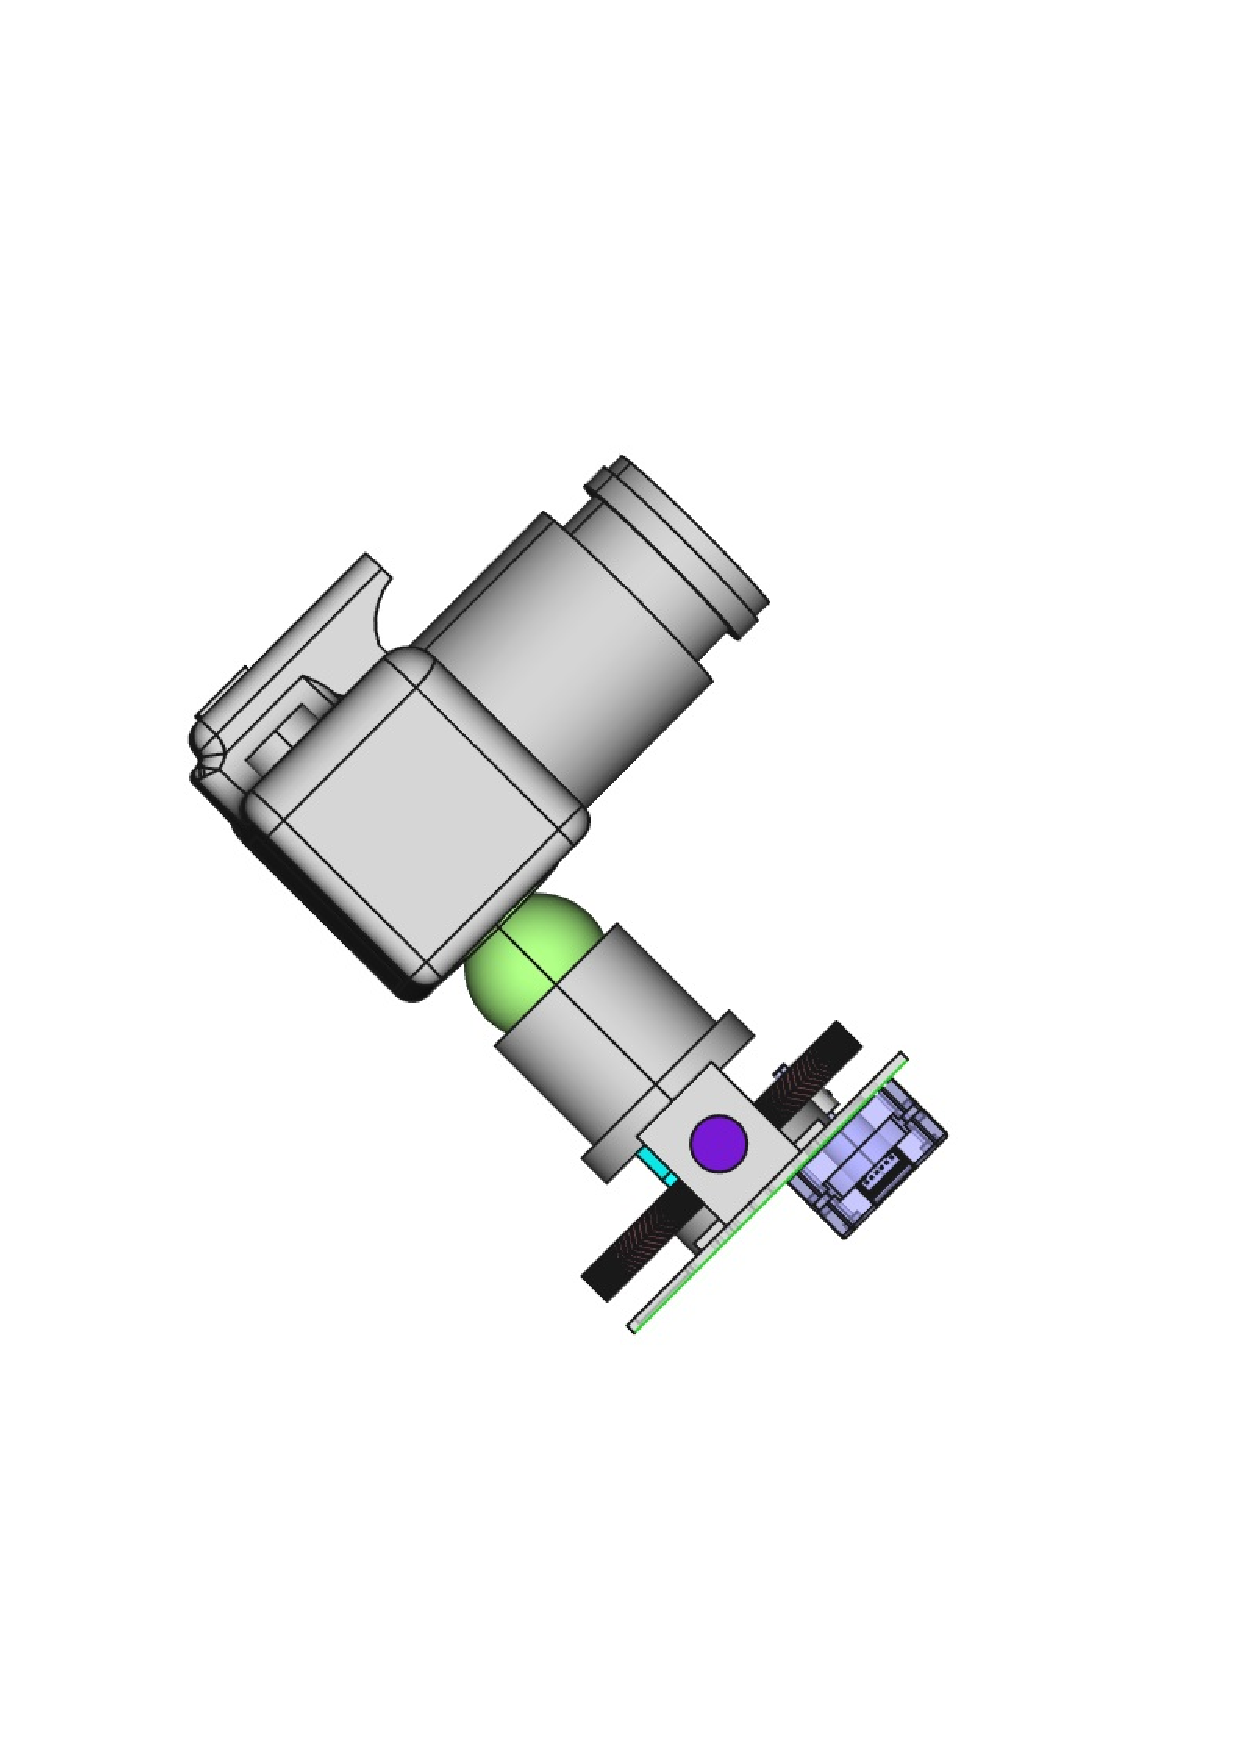
\includegraphics[trim=0 80 0 200, clip, angle=-45, origin=c, width=0.7\linewidth]{images/motors/cm_render_45_3.pdf}
		}
		
		\node (o1) at (-0.8, 0.7) [draw=black, circle, fill=cyan, inner sep=1.2pt] {};
		\node (o2) at (-0.15, -0.9) [draw=black, circle, fill=blue, inner sep=1.2pt] {};
		
		\draw [line width=1.5pt, color=cyan, arrows=->] (o1) -- +(0, 1) {};
		\draw [line width=1.5pt, color=cyan, arrows=->] (o1) -- +(1, 0) {};
		\draw [line width=1.5pt, color=blue, arrows=->] (o2) -- +(0, 1) {};
		\draw [line width=1.5pt, color=blue, arrows=->] (o2) -- +(1, 0) {};
		
		\node (cm) at (1, 1.3) [draw=black, fill=red, inner sep=1.6pt, circle] {};
		
		\node (o1t) at ($(o1) - (0, 0.2)$) [draw=none] {$O_1$};
		\node (o2t) at ($(o2) - (0.1, 0.3)$) [draw=none] {$O_2$};
		\node (cm1t) at ($(cm) + (0, 0.2)$) [draw=none, scale=0.8, color=cyan] {$(67.4, 44.6)_{O_1}$};
		\node (cm2t) at ($(cm) - (0, 0.2)$) [draw=none, scale=0.8, color=blue] {$(32.4, 123.6)_{O_2}$}; 
	\end{tikzpicture}
	\caption{The two origins used for the computations: $O_1$ is on the camera, $O_2$ is on the gear; this results in two different coordinates for the c.m.}
	\label{fig:cmorigins}
\end{figure}

The vertical offset is given from the height of the ball-head and the support between the ball-head and the gear. The horizontal offset is measured as the distance from the axis of rotation, which is the point where the camera is screwed at the ball-head, and the origin of the camera. 

So, the new centre of mass is:

\begin{align*}
	x_{cm} & = 67.4 - 35 \\
		   & = 32.4 mm \\
	z_{cm} & = 37.4 + 79 \\
		   & = 123.6 mm
\end{align*}

We can think of the system as a \textbf{pulley}: the camera tries to rotate it, while the motor applies an opposing force. When the system is parallel to the ground, the parallel component of the force with reference to the \textit{top} plane exercised by the camera is $0$; when the plane is perpendicular to the ground is maximum. We can approximate the camera with its centre of mass.

let's call this the \textbf{moment of force M}.

$$ M = \frac{\textnormal{distance between c.m. and centre of gear} \cdot F}{\textnormal{transmission  ratio}}$$

where $F$ is the weight force and \textit{transmission ratio} is the transmission ratio between the two gears. Only the parallel component of the weight force should be considered, $F_{\parallel}$, as shown in figure \ref{fig:moment}. So the final computation is:

$$ \frac{ \left[ (0.265 + 0.430)\cdot 9.81 \right] \cdot \sin\alpha \cdot 12.78}{\frac{126}{17}}$$
\\
$12.78$ is the distance in cm of the c.m. from the centre of the gear: $\sqrt{32.4^2 + 123.6^2}$. 

Considering various values of $\alpha$, this gives the following chart \ref{fig:momentchart}:

\begin{figure}[H]
	\centering
	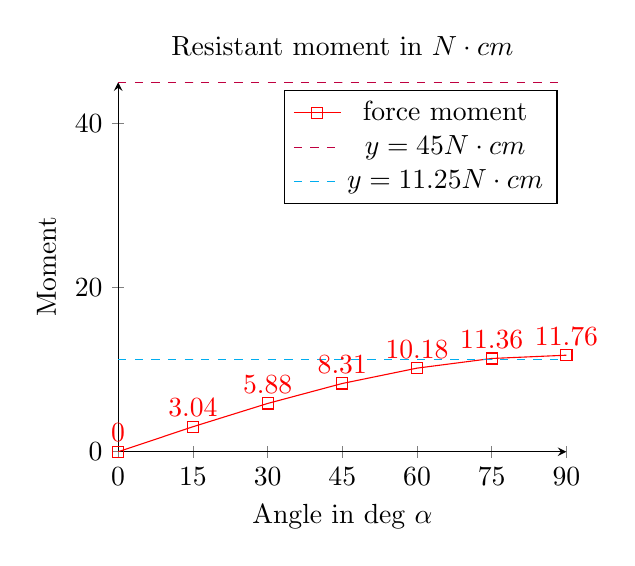
\begin{tikzpicture}
		
		\begin{axis}[
			width=0.6\textwidth,
			title={Resistant moment in $N\cdot cm$},
			xlabel={Angle in deg $\alpha$},
			ylabel={Moment},
			xtick={0, 15, 30, 45, 60, 75, 90},
			xmin=0, xmax=90,
			axis lines = left,
			%			ytick={0, 250, 350, 500}
			]
			\addplot [ 
			domain=0:90, 
			color=red,
			mark=square, 
			samples = 7,
			nodes near coords, 
			xtick={0, 15, 30, 45, 60, 75, 90}, ]
			{((0.695 * 9.81)*sin(x)*12.78)/(126/17)}; 
			\addlegendentry{force moment}
			
			\addplot[
			domain=0:90,
			color=purple,
			dashed
			]{45};
			\addlegendentry{\( y = 45 N\cdot cm \)}
			
			\addplot[
			domain=0:90,
			color=cyan,
			dashed
			]{((45/4)};
			\addlegendentry{\( y = 11.25 N\cdot cm\)}
		\end{axis}
		
	\end{tikzpicture}
	\caption{This chart shows the moment generated by the camera at various inclination, the torque generated by the motor, and the torque generated by the motor divided by 4. }
	\label{fig:momentchart}
\end{figure}

The two horizontal lines, $y=45$ and $y=11.25$, are the torque of the motor. The second in particular is the moment divided by 4, for reasons that will be explained in the following subsection, since that number is obtained because of the technique used to drive the motor, \textit{microstepping}. The graph shows that, except above $\alpha = 75^{\circ}$ of inclination, the motor can move the camera. 

\begin{figure}[h]
	\centering
	\begin{tikzpicture}		
		\pgftext[at=\pgfpoint{0cm}{0cm},left,base]
		{\inctrimpic[1]{images/motors/cm_render_front_0.pdf}};
		% ...
		\node (G) at (6.4,3.8)
		[circle,draw=black,inner sep=2pt,fill=red]
		{};
		\draw[gray,dashed,line width=1pt] (G) circle (2.75cm);
		\draw [line width=1pt, color=black] 
		(G)+(-3, 0) -- +(2, 0) ;
		\draw[thick, color=orange] (G)+(-2,0) arc (180:105:2cm);
		\draw[thick, color=orange] (G)+(-1,0) arc (180:18:1cm);
		\draw[thick, color=orange] (G)+(-1.1,0) arc (180:18:1.1cm);
		\draw[line width=2pt,shorten <=6pt, color=blue]
		(G)+(0,4) -- +(0,-4)
		node[draw=none,inner sep=0pt,fill=none] (V1)
		{};
		%		\node (X) at (7.1, 4.2)
		%		[draw=none]
		%		{};
		\draw[line width=2pt,arrows=->, color=red]
		(G) -- +(-0.7,2.8)
		node[below, inner sep=2pt,fill=black, circle] (CM)
		{};
		\node at (CM) [draw=none, left=0.1cm] {Centre of mass};
		\node at (G) [draw=none, above left=1cm] {\color{orange}$\theta$};
		\node at (G) [draw=none, above left=0.3cm] {\color{orange}$\theta'$};
		
		\draw[line width=1.5pt, arrows=<->, color=green]
		(CM) -- +(0.7, 0)node[draw=none] (D) {};
		
		\path (V1)
		to node [above left=.6cm]
		{Axis of rotation} (G);
		%		\path (X)
		%		to node [left=0.2cm]
		%		{Lever arm} (CM);
		
		\draw[line width=1pt,arrows=->, color=red]
		(G) -- +(2.6,0.8)
		node[inner sep=1.5pt,fill=black, circle] (CMa)
		{}; %alternative center of mass
		\node at (CMa) [draw=none, right=0.1cm] {$CM'$};
		\draw[line width=1pt, arrows=<->, color=green]
		(CMa)+(0,0.1) -- +(-2.6, 0.1) node[draw=none] (D) {};
	\end{tikzpicture}
	\caption{This image represents the angles of the camera respect to the \textit{top} plane, if the camera is tilted on the ball-head on various position ($\theta$, $\theta'$). The tilt pushes the centre of mass of the camera closer or further from the axis of rotation. The double green arrow represents the horizontal distance of the c.m. from the axis of rotation. }
	%		Other values are available in table \ref{tab:angles}.}
\label{fig:theta}
\end{figure}


Until now, the angle $\beta$ of the camera on the ball-head used for the computation has been 0.
But we can consider any ball rotation: changing the angle on the camera brings the c.m. closer to the axis of rotation, or furthers it away, as shows figure \ref{fig:theta}.

Although these computations are not and will not be taken into consideration, it is still interesting to cite the possibility of improving the graph shown in \ref{fig:momentchart} by taking them into account, so a brief description of how to get these values is provided.

To compute the distance of the c.m. considering $\beta$, it is useful to introduce $\theta$, the angle between the camera and the \textit{top} plane. The c.m., as rotates around the centre of the ball in the ball-head, describes a circumference. Again, for simplicity, it is possible to only considering a 2D plane, and not a whole sphere. 

Knowing the position of the c.m. of the camera using the origin at the centre of the gear, it is possible to measure the distance between the c.m. and the centre of the ball in the ball-head. This gives the radius of the circumference introduced above. The radius is shown in figure \ref{fig:theta} (the red arrow) and more explicitly in figure \ref{fig:radius}.

The angle $\theta$ for $\beta = 0$ is given from:

$$\theta = \arcsin \frac{r_{\perp}}{\sqrt{r_{\perp}^2 + r_{\parallel}^2}} $$

where $r_{\perp}$ is the perpendicular component of $r$ w.r.t. the \textit{top} plane, or $r \cdot \sin \theta$, and $r_{\parallel}$ is the parallel component of $r$ w.r.t. the top plane, $r \cdot \cos \theta$. 

\begin{figure}[h]
	\centering
	\begin{tikzpicture}
		\pgftext[]{
			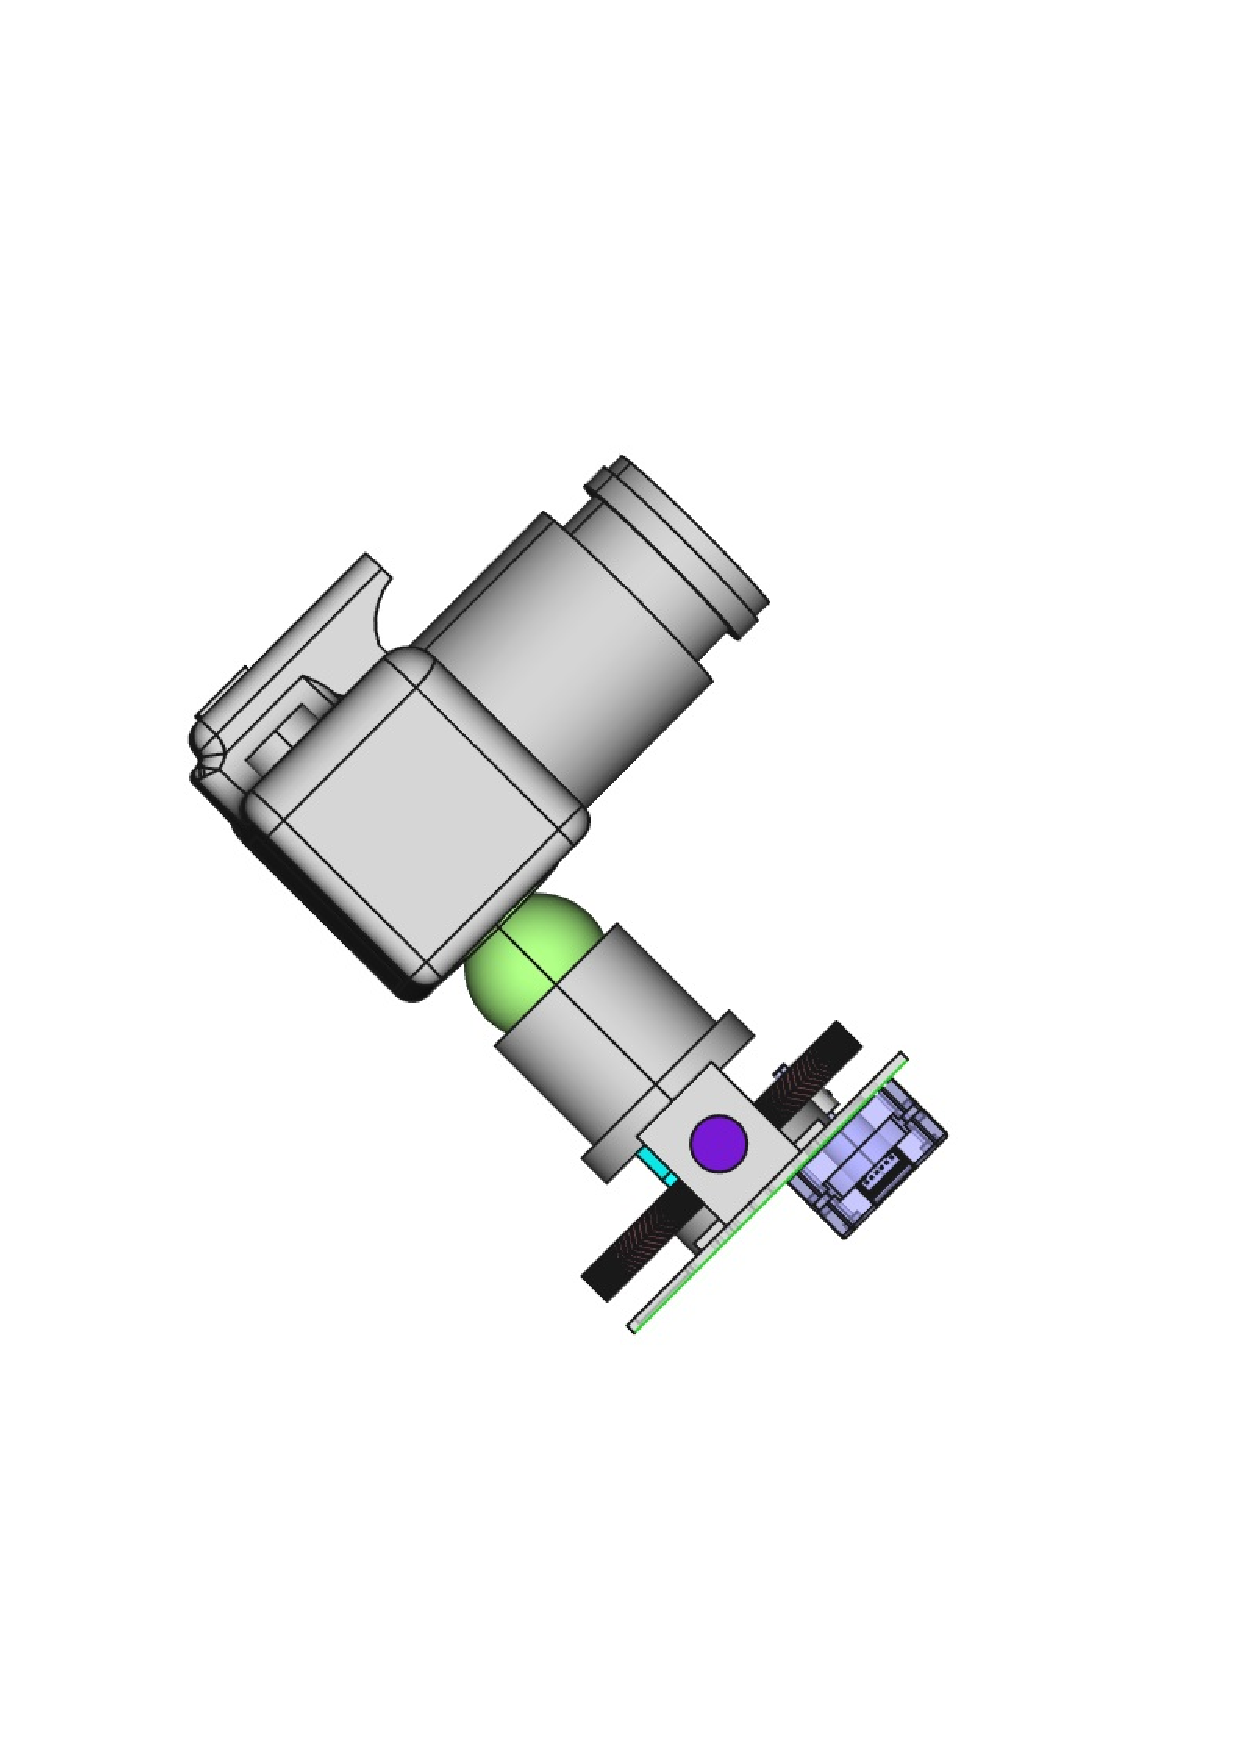
\includegraphics[trim=0 80 0 200, clip, angle=-45, origin=c, width=0.7\linewidth]{images/motors/cm_render_45_3.pdf}
		}
		
%		\node (o1) at (-0.8, 0.7) [draw=black, circle, fill=cyan, inner sep=1.2pt] {};
		\node (o2) at (-0.15, -0.9) [draw=black, circle, fill=blue, inner sep=1.2pt] {};
		
%		\draw [line width=1.5pt, color=cyan, arrows=->] (o1) -- +(0, 1) {};
%		\draw [line width=1.5pt, color=cyan, arrows=->] (o1) -- +(1, 0) {};
		\draw [line width=1.5pt, color=blue, arrows=->] (o2) -- +(0, 1) {};
		\draw [line width=1.5pt, color=blue, arrows=->] (o2) -- +(1, 0) {};
		
		\node (cm) at (1, 1.3) [draw=black, fill=red, inner sep=1.6pt, circle] {};
		
		\draw[arrows=->, line width=2pt, color=red] (o2) -- (cm) node[midway, below, scale=1.5, draw=none]{$r$} ;
		\draw[line width=1.5pt, arrows=->, color={rgb:red,4;green,2;yellow,1}]
		(cm) -- +(0, -2.1) node[draw=none, right] {$r_{\perp}$};
		\draw[line width=1.5pt, arrows=->, color=purple] (cm) -- +(-1.15, 0) node[left, draw=none] {$r_{\parallel}$};
		
	\end{tikzpicture}
	\caption{The distance from the centre of the gear and the c.m. of the camera; this also describe the radius of a circumference. In this figure are also shown its components.}
	\label{fig:radius}
\end{figure}


Finally, the torque is given by $r_{\parallel}\cdot F$, where $r_{\parallel}$ is the horizontal distance from axis, and $ F = m\cdot g = (430+265)\cdot9.81 $.

To conclude, it is possible to compute a more realistic moment of the force considering also a rotation $\theta$ of the camera: for different values of $\theta$ correspond different values of $r_{\parallel}$, i.e. the distance between the c.m. and the centre of the gear does not depend only on $\alpha$, but also on $\theta$. 

\subsection{Micro-stepping}

A stepper motor, such as the ones used in this project, is a motor that moves a shaft through the use of electromagnets. More specifically, there is a rotating, permanent magnet, called \textit{rotor}, and a \textit{stator}, which is a static part that is magnetized when the current passes through it \cite{steppermotors}. Every time the stator is magnetized, the rotor rotates. The rotation made by the rotor is called a \textbf{step}, and is a fixed amount of degrees; all the motors used for this project require 200 steps to make a complete rotation.
\\
\\
However, the time required for the big \textit{top} gear to make a complete rotation is more than $80,000$ seconds, a \textbf{sidereal day}, as explained in section \ref{sec:intro}. 

Considering the transmission ratio of the \textit{top} gears, which is $\frac{126}{17} \approx 7.4$, this means that $200 \cdot 7.4 $ steps of the small gear are needed to completely rotate the big gear. This rotation has to take the same amount of time of a sidereal day, i.e. 86164 seconds, which means that a step needs to take place every $\frac{86164}{200\cdot 7.4} \approx 58 $ seconds. But according to the \textit{500 rule}, this time is too long for the star tracker to be useful, because a star trail will appear during the wait time between the steps. 

Fortunately, there are some ways to augment the number of steps, reducing the wait time to an acceptable duration. 

To begin with, a \textbf{bipolar stepper motor}, such as the ones used in this project, has two stators, hence the motor is driven with two phases. There are several ways to drive the motor: \textit{single-phase step}, \textit{full-step}, \textit{half-step}. The core idea is that for every phase the current flows through one or two stator in a direction, then flows in the other rotor(s), then again in the first rotor(s) in the opposite direction and finally in the second rotor(s) in the opposite direction. The simplified schematic of a bipolar motor is shown in figure \ref{fig:schembipolar}, and the above modes are summarized in table \ref{tab:controlmodes}.

\begin{figure}[h]
	\centering
	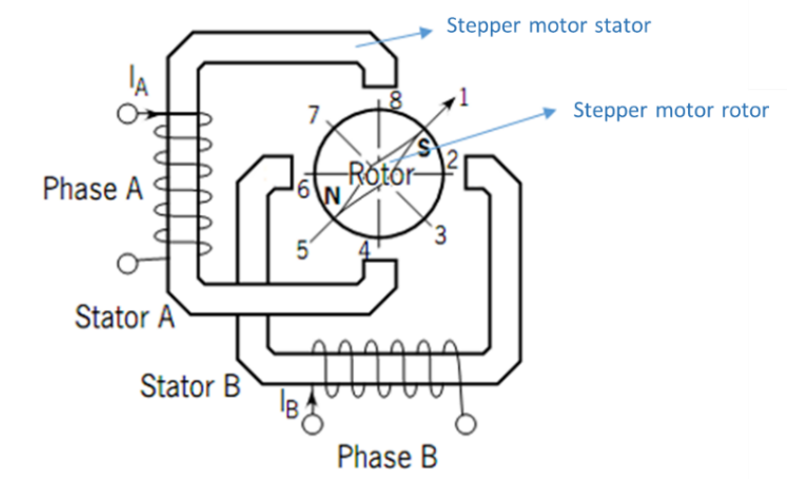
\includegraphics[width=7cm]{images/motors/schemabipolarmotor.png}
	\caption{Simplified Schematic of a Bipolar Stepper Motor \cite{steppermotors}.}
	\label{fig:schembipolar}
\end{figure}

\begin{figure}[h]
	\centering
%	\bgroup
	\def\arraystretch{1.5}
	\bfseries
	\begin{tabular}{|c|c|c|}
		\hline
		\thead{Stepping mode} & \thead{Sequence} & \thead{Electrical stepping position} \\
		\hline
		Single-phase step & $A > B > \bar{A} > \bar{B}$ & $8 > 2 > 4 > 6$\\
		\hline
		Full step & $AB >  \bar{A} B > \overline{AB} > A\bar{B}$ & $1 > 3 > 5 > 7$ \\
		\hline
		Half-step & $AB > B > \bar{A}B > \bar{A} > \overline{AB} > \bar{B} > A\bar{B} > A $ & $1>2>3>4>5>6>7>8$ \\
		\hline
	\end{tabular}
	\caption{Stepper Motor Control Modes \cite{steppermotors}}
	\label{tab:controlmodes}
	
\end{figure}

If the half-step mode is used, the steps needed double, allowing to halve the wait time: $\frac{58}{2} = 29$ seconds. 

But it is also possible to use the \textbf{microstepping} technique, which consists of dividing a single step in multiple steps: for example, using two microsteps the number of steps is once again halved and the wait time can be brought down to about 14 seconds. 

Normally, the impulse to the stator is digital, meaning there is current or there is not. With microstepping, the impulse is sent in a wave form, thus the step is gradual as the amount of current increases or decreases. A sinusoidal wave form is obtained through \textbf{PWM}, pulse-width modulation \cite{microstepping}. 
\\
\\
Microstepping solves the problem of obtaining a smooth, slow rotation, but since a smaller amount of current is used, less torque is produced by the motor. For simplicity, let's assume that the torque is linearly proportional to the amount of current \footnote{This is a generous assumption, since it is not obvious: see \cite{torquevoltage}.}. Fortunately, according to the computation of the previous subsection, as shown in chart \ref{fig:momentchart}, even diving by 4 - i.e. 4 microsteps - the amount of torque is still enough to move the camera below $75^{\circ}$ of inclination. Thus, a \textbf{2 microsteps} step can be safely used. 

\newpage
\section{Electronics}
In this section, all the electronic components, the electronic scheme and some energy considerations are discussed. 

The table below \ref{tab:elecsummary} provides a summary of all the components used, excluding the motor, which specifications where introduced in table \ref{tab:topseq}.

\begin{table}[H]
	\centering
	\def\arraystretch{1.5}
	\begin{tabularx}{\linewidth}{|X|c|c|X|}
		\hline
		\textbf{Name} & \textbf{Voltage} & \textbf{Current} & \textbf{Description} \\
		\hline
		Raspberry Pi 3B+ & 5V & 2.5A & The Raspberry connects all the sensors actuators, and provides computation capabilities. \\
		\hline 
		GY-521 MPU6050 & 3V & 3.9mA & accelerometer to read \textit{top} plane inclination \\
		\hline
		MT3608 & 2V-24V & 2A & DC-DC step up booster \\
		\hline
		u-blox NEO-6M GPS & 3V & 45mA & gps chip to get date and position \\
		\hline
		Adafruit ICM20948 & 1.8V & 3.11mA  & IMU, used to orient the startracker towards the north \\
		\hline
	 	L298N DC motor driver & 5V & 4A & motor driver (operates at 5V, can manage an input voltage to drive the motor up to 48V) \\
	 	\hline
 		L9110 H-bridge module & 2.5V & 1.6A & motor driver \\
	 	\hline
	 	led & 2V & 20mA & led \\
	 	\hline
	 	resistor & & & $560 \Omega$ resistor for the led \\
	 	\hline
	 	on-off button & & & button to read digital input \\
	 	\hline
	 	unipolar switch & max 250V & 2A & on-off switch between battery and motors \\
	 	\hline
	 	TP4056 & 4.5V-5.5V & 1A & microusb battery charger module \\
	 	\hline
	 	LIPO-2200mAh & 3.7V & & battery for the motors \\
	 	\hline
	\end{tabularx}
	\caption{Summary of all the electronic components used, except the motors.}
	\label{tab:elecsummary}
\end{table}

\begin{figure}[H]
	\centering
	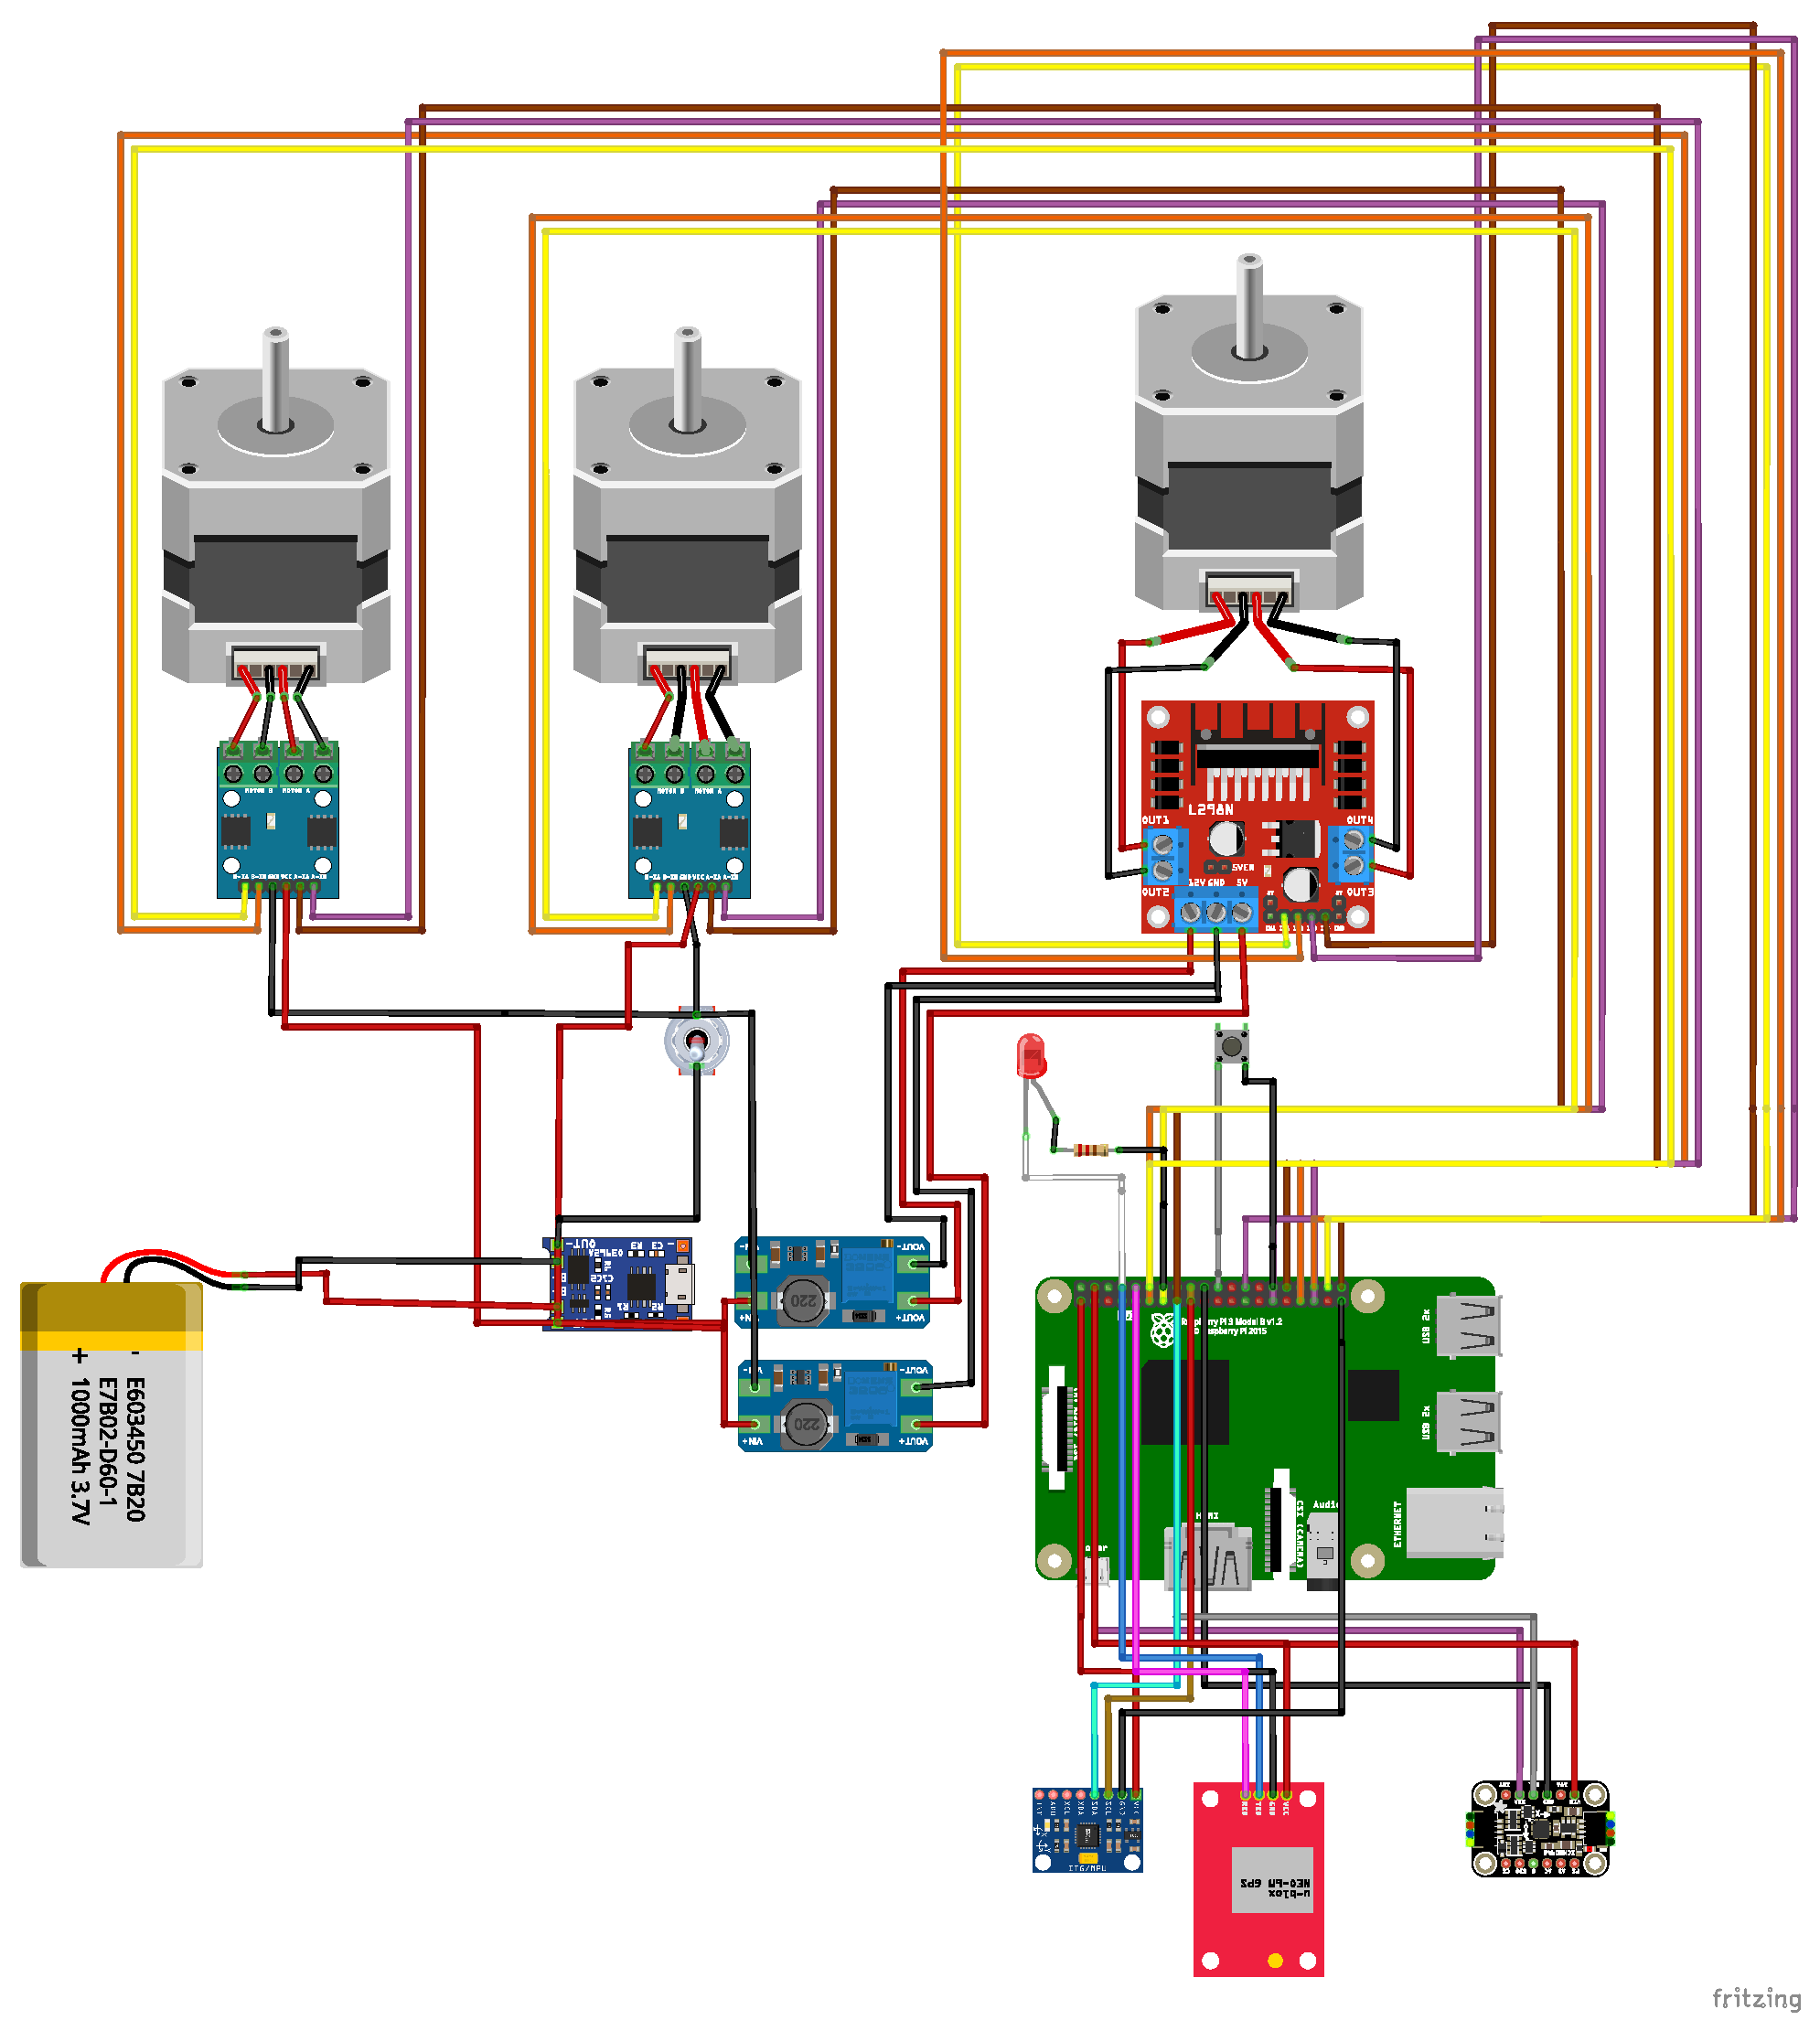
\includegraphics[width=\linewidth]{images/electronic/schema.pdf}
	\caption{The electronic scheme.}
	\label{fig:elecfullscheme}
\end{figure}

Given the nature of the simple logic required by the sensors and actuators, a microcontroller such as an Arduino would have been a more suitable choice; it would have also provided additional improvements such as less energy consumption and a finer control, due to the lack of an operating system that can introduce some lag. 

However, the Raspberry was already available to me, so a microcontroller was an additional purchase that could have been avoided.  Furthermore, using the Raspberry it is possible to develop an additional image-based alignment technique, for which a microcontroller is not suitable, due to the lack of processing power. In this sense, the raspberry makes the project more "future proof". 

While the sensors, the led-resistor and the on-off button are directly attached to the Raspberry, the motor circuitry is slightly more complicated. 

There are two smaller motors, the Nema 17HS4023, and a bigger one, the 17HS15, as showed in table \ref{table:motor}. Since the first motor require less voltage, they are attached to drivers (L9110) which are connected directly to the battery. 

The second motor, however, is attached to a DC-DC converter that steps up the output voltage of the battery, to around 12V. So, the battery is connected to this module, which is connected to a more powerful driver (L298N) which is finally attached to the motor. A second DC-DC converter is also connected from the battery to the driver; while the first provides the energy for the motors, the second powers the driver itself. 

The battery is connected to a charger circuit (TP4056); hence, the motor drivers are not directly connected to the battery as previously stated, but are actually connected to this charger circuit. 

These connections are summarized in figure \ref{fig:batterycircuit}.

\begin{figure}[h]
	\centering
	\begin{tikzpicture}
		\pgftext[]{
			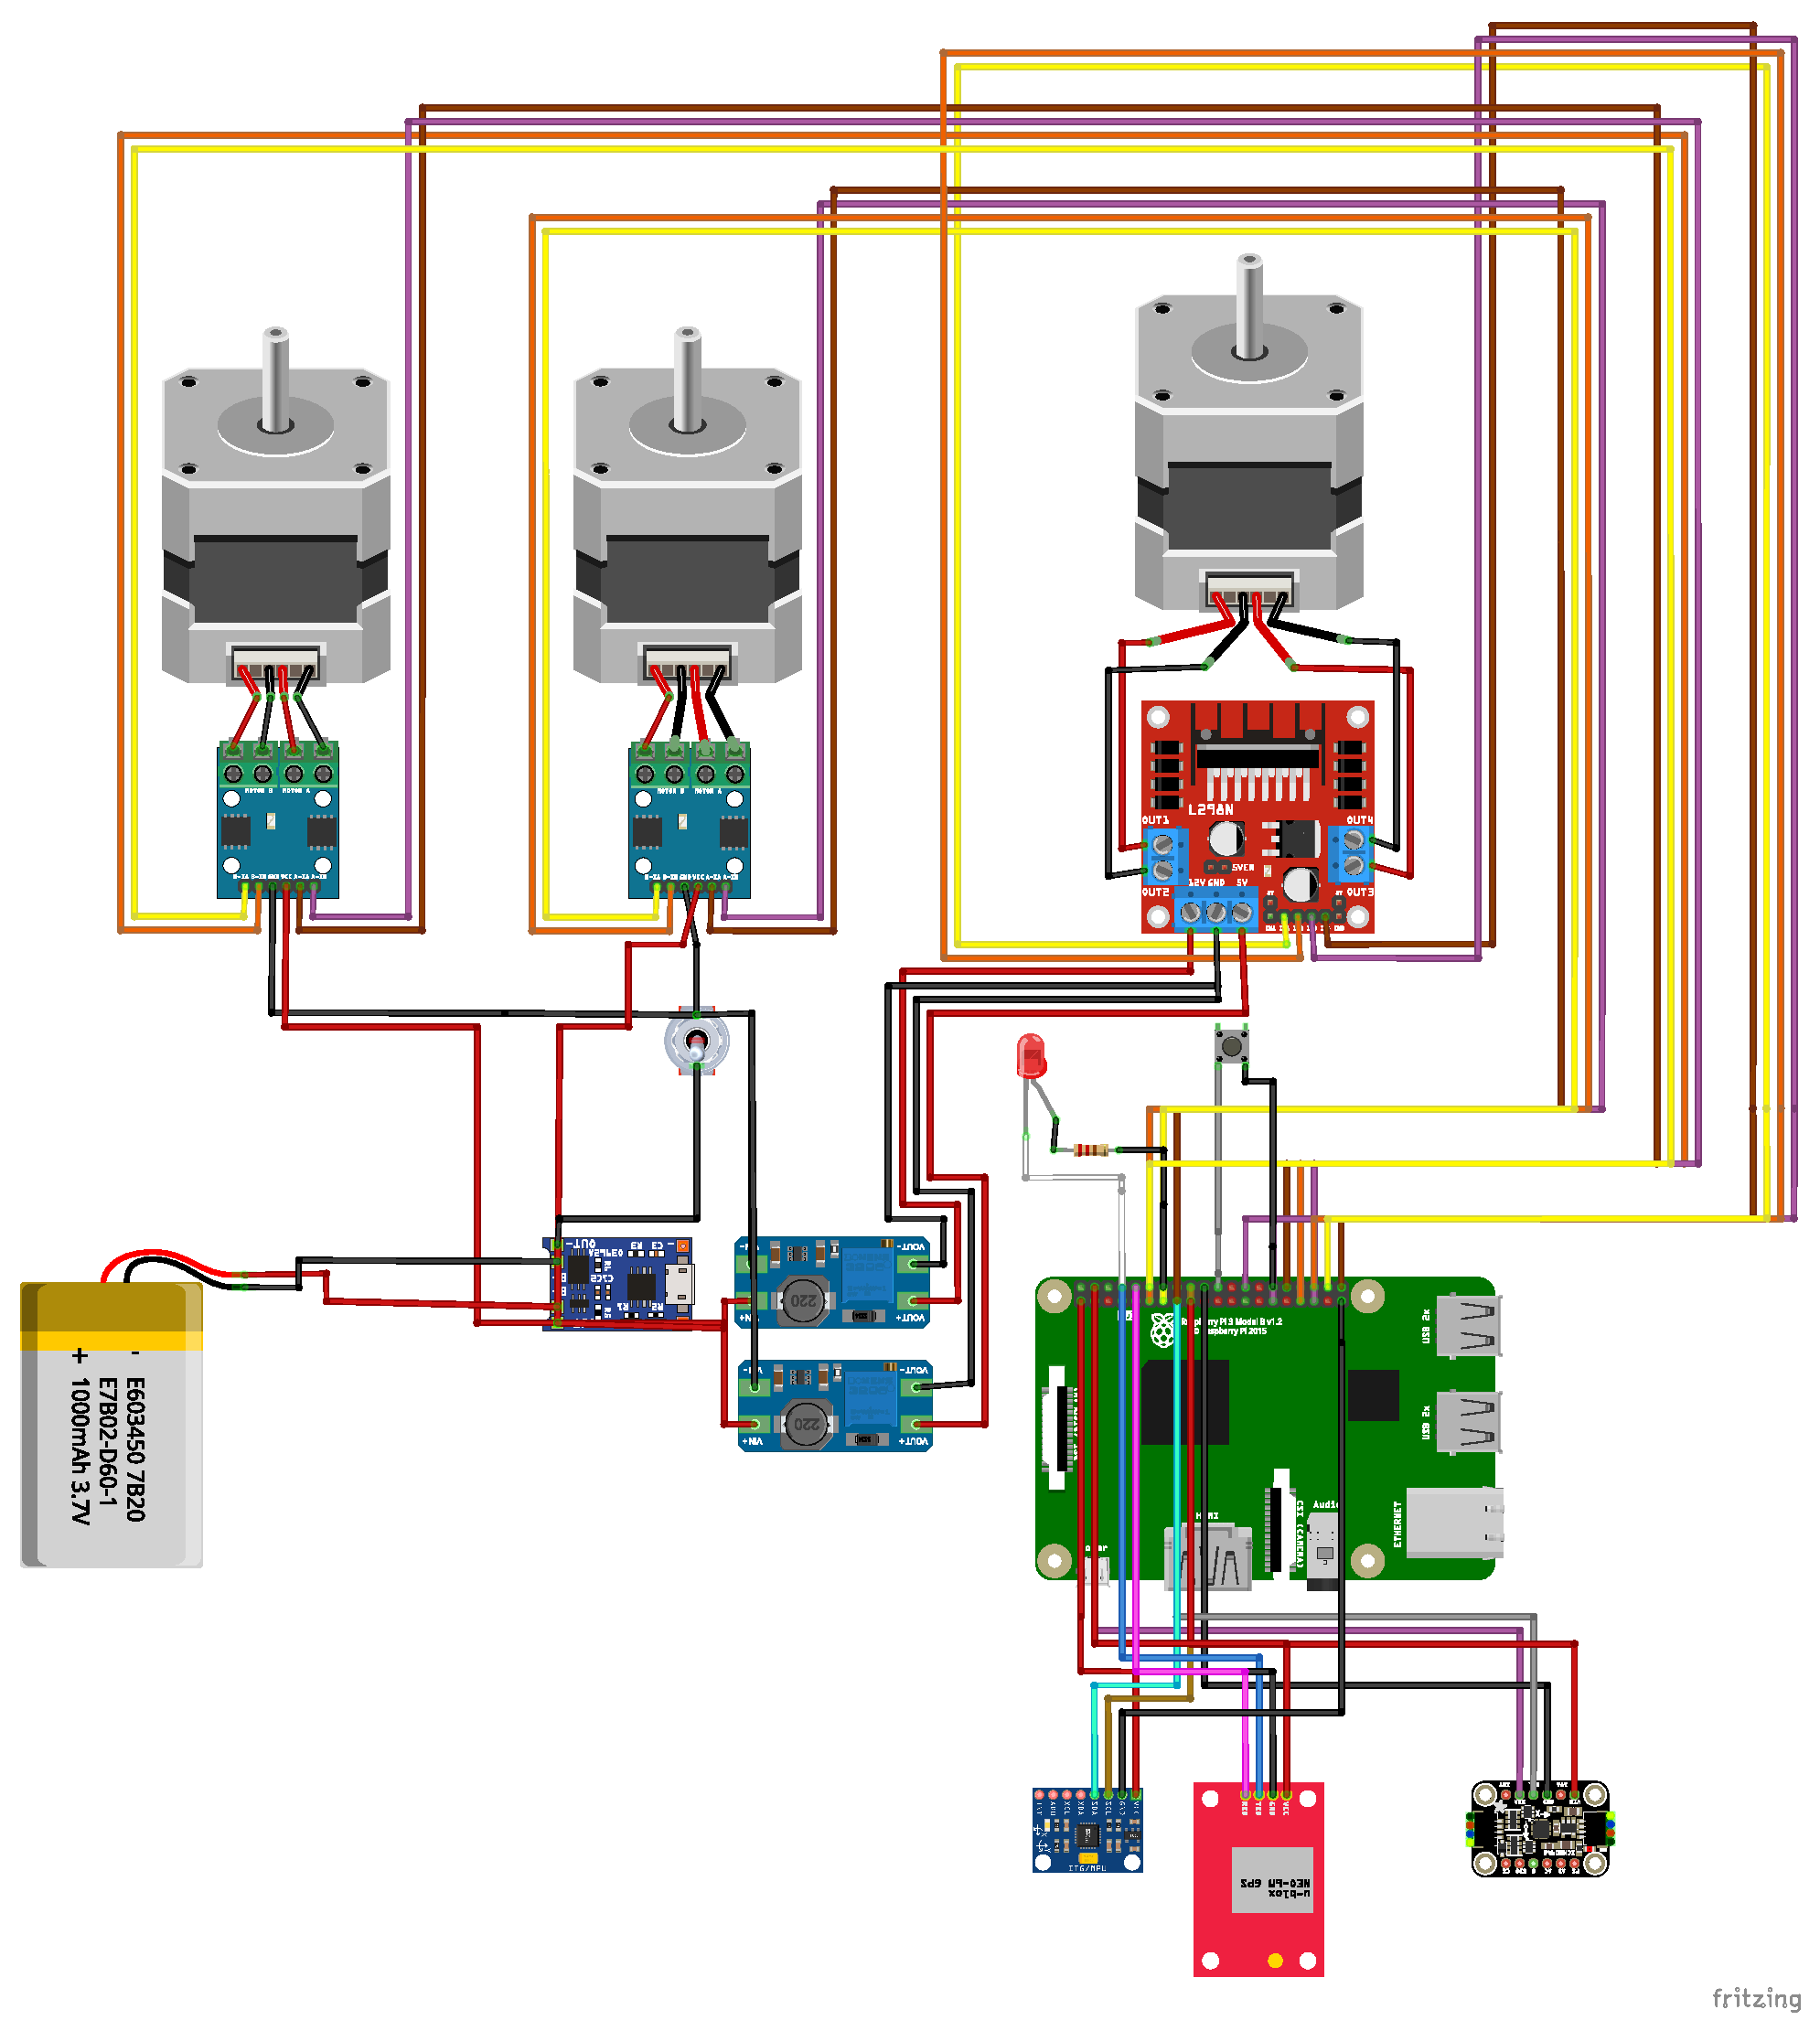
\includegraphics[width=0.8\linewidth, trim=0 250 430 350, clip,]{images/electronic/schema.pdf}
		}
		\draw[line width=1pt, blue] (1.2,-1.6) ellipse (0.8 and 1.1);
		\draw[line width=1pt, green] (3.3,-1.6) ellipse (1.2 and 0.8);
		
	\end{tikzpicture}
	\caption{Battery and motor electric circuit: the battery is connected to a charger module, circled in \textcolor{blue}{blue}; from here, 4 red wires exit and are connected to the two DC-DC step up modules, one of which is circled in \textcolor{green}{green} (the other one is below), and the two motor driver at the top of the image. The charger module, DC-DC and motor drivers are also all connected through the on-off switch at the centre of the image, to disconnect the load from the battery. Finally, the DC-DC modules are connected to another motor drive, not included in this image.}
	\label{fig:batterycircuit}
\end{figure}

\subsection{Communication protocols}\label{sec:communication}
The various sensors such as the gps and the IMU modules are connected directly to the Raspberry, to which communicate with 2 protocols:

\begin{itemize}
	\item \textbf{I2C protocol};
	\item \textbf{UART protocol}.
\end{itemize}

The Raspberry provides a bus for each of these communication protocol: I2C bus is accessible through GPIO pins 2 and 3, while UART through pin 14 and 15. 

Here there is the list of each electronic component and its communication protocol:
\begin{itemize}
	\item GY-521: I2C;
	\item NEO 6M GPS: UART;
	\item Adafruit ICM20948: I2C.
\end{itemize}

The rest of the electronic components (led, motor drivers...) are controlled only setting on or off the pins to which they are connected.

However, there are two I2C devices and one bus; but in the Raspberry Pi, is possible to define a software I2C bus using two generic GPIO pins \cite{i2cadafruit}. Thus, while the Adafruit chip is connected to the GPIO pins 2 and 3, the GY-521 is connected to the GPIO pins 23 and 24. 

This is obtained through the \textbf{Device Tree overlay feature} of the Raspberry's firmware. An overlay purpose is to modify the kernel live tree; the device tree describes the hardware of a system, using a tree data structure. To configure the overlays, the file \texttt{/boot/config.txt} must be edited. In the case of the software I2C, two lines were added:

\begin{lstlisting}[language=Bash, caption={Additional lines in \texttt{/boot/config.txt} to add a software I2C overlay.}]
dtoverlay=i2c-gpio #define the overlay
dtoverlay=i2c-gpio,i2c_gpio_sda=23,i2c_gpio_scl=24 #specify the pins
\end{lstlisting}

\subsection{Energy power computation}
Knowing how much energy the system consumes, allows to estimate the battery duration, hence for how long it is possible to use the system.

To begin with, let's compute how much power the battery can provide working for 1 hour:

$$ P = V\cdot I \cdot 1h  = 3.7 \cdot 2200Ah = 8.14 Wh $$

Using the same method, it is possible to compute the power required by the motors attached to the battery.

The first motor, the bigger one, can be run at $1.5A$, and $12V$, thus giving $18Wh$.

The second and the third run at $1A$ and $3.7V$ each, which gives $3.7Wh$; multiplying by 2 the total is $7.4Wh$. 

The driver for the bigger motor, the L298N, runs at around $36mA$ and $5V$, which gives $0.18Wh$; the other two drivers are not alimented through to the battery, but the boards are powered by the Raspberry.

So, the total time the battery can operate under this load is given from:

$$ \frac{8.14}{18 + 7.4 + 0.18} \cdot 60 \approx 19 \textnormal{minutes} $$

Now, assuming that the DC-DC modules have an efficiency of 80\% \cite{mtspecs} to boost the input voltage to $12V$, 
the total is $19\cdot 0.8 = 15.2 $ minutes. Since the second module output is $5V$, its efficiency should be around 90\%, resulting in $15.2\cdot 0.9 = 16.7$ minutes, which is enough for taking e.g. two 5 minutes exposure pictures.

\subsubsection{Problems of using MT3608 modules}
These modules are DC-DC voltage booster: their purpose is to increase the input voltage. But this is achieved decreasing the current: this means that the bigger motor is driven with a much low current than the needed $1.5A$ in its specification. In fact, stepper motor torque is proportional to the current, and stepper motors should be driven with constant current \cite{steppermcurrent}.

According to \cite{mteffspec}, which tested the efficiency of the module, applying a $2A$ input resulted in a $0.4A$ of output, or about 20\% of the input, with the module configured to boost $5V$ to $12V$.

\subsubsection{Raspberry Pi power consumption}
Assuming the Raspberry Pi 3B+ consumes around $5W$ while not in idle \cite{powerbenchmark}, it is possible to estimate how much power requires considering also the attached electronic components. 

For all the components, the voltage and current are listed, and the computation is straightforward using the formula $P=V\cdot I$ introduced before:

\begin{itemize}
	\item GY-521: $3 \cdot 0.0039 = 0.012W$
	\item NEO-6M: $3 \cdot 0.045 = 0.135W$
	\item Adafruit ICM20948: $1.8 \cdot 0.0031 = 0.006W$
\end{itemize}

The total of the watts above is $0.513W$. There is another component though, the $560\Omega$ resistor and led, for which another two formulae are needed:

$$ P = \frac{V^2}{R} \qquad\qquad I = \frac{(V_i - V_o)}{R}$$

$R$ is known, is the resistance of the resistor and its value is $560\Omega$; $V_i$ is the voltage supplied from the Raspberry, $5V$, while $V_o$ is the voltage at which the led operates: $2V$. Thus, the value at which the led operated, I, is $\frac{5-2}{560} = 5.3mA$.

From this value, it is possible to compute the power used by the led: $2 \cdot 0.0053 = 0.011W$ and the resistor: $P = \frac{(5-2)^2}{560} = 0.016W$.

Thus, the total power consumption for the raspberry is $\approx 5.53 W$.

\subsection{Magnetic calibration}\label{sec:iron_calib}
A magnetometer is a sensor that can measure the strength of a magnetic field. Unfortunately, what is actually measured is a combination of all the local magnetic fields; this is particularly problematic if the magnetometer is needed to find the Earth's magnetic north. 

\begin{figure}[H]
	\centering
	\subfigure[No distortions]{
		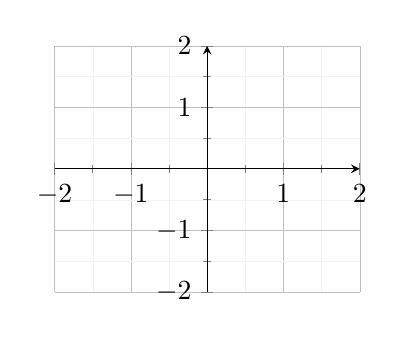
\begin{tikzpicture}
   			\begin{axis}[
				width=0.45\textwidth,
				xmin=-2, xmax=2,
				ymin=-2, ymax=2,
    			minor tick num=1,
				grid=both,
				grid style={line width=.05pt, draw=gray!10},
				major grid style={line width=.1pt,draw=gray!50},
				axis lines=middle,
				]
				
				\coordinate (O) at (axis cs: 0, 0); 
				\node[fill=white,circle,inner sep=0pt] (O-label) at ($(O) - (25,25)$) {$O$};
				\draw[color=blue] (O) circle [radius=100];
				
			\end{axis}
		\end{tikzpicture}
	}
	\subfigure[Hard and soft iron distortions]{
		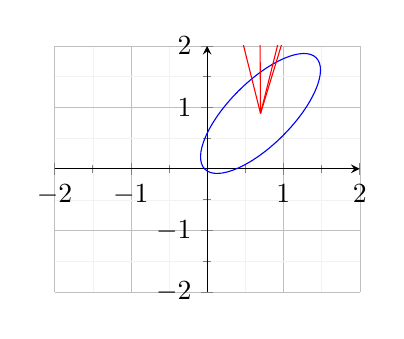
\begin{tikzpicture}
			\begin{axis}[
				width=0.45\textwidth,
				xmin=-2, xmax=2,
				ymin=-2, ymax=2,
				minor tick num=1,
				grid=both,
				grid style={line width=.05pt, draw=gray!10},
				major grid style={line width=.1pt,draw=gray!50},
				axis lines=middle,
				]
				\coordinate (O) at (axis cs: 0, 0); 
				\coordinate (C) at (axis cs: 0.7, 0.9); 
				\node[fill=white,circle,inner sep=0pt] (O-label) at ($(O) - (25,25)$) {$O$};
				\draw[color=blue, rotate=45] (C) ellipse({1cm} and {0.4cm});
				\draw[color=red, rotate=45] (C) -- +( 1cm,  0)     {};
				\draw[color=red, rotate=45] (C) -- +(-1cm,  0)     {};
				\draw[color=red, rotate=45] (C) -- +(   0,  0.4cm) {};
				\draw[color=red, rotate=45] (C) -- +(   0, -0.4cm) {};
				]
			\end{axis}
		\end{tikzpicture}
	}
	\caption{Effects of the magnetic disturbances: the second figure is shifted from the centre (hard iron), and forms an ellipse (soft iron distortion).\\}
\end{figure}

If the magnetometer is rotated around an axis, and the read magnetic field is plotted on a 2D plane, the plot should form a circle, assuming no disturbances are present. 
There are two types of magnetic disturbances \cite{vectornav}:
\begin{itemize}
	\item \textbf{soft iron}: this type of distortion is commonly caused by metals and other sources such as batteries; they tend to stretch the plot, making it elliptical;
	\item \textbf{hard iron}: these disturbances come from other magnetic fields nearby, and cause the plot to be off-centre.
\end{itemize}

After collecting data about the magnetic field around the magnetometer rotating it, it is possible to analyse the data to compute the necessary correction to calibrate the magnetometer, and allow it to find the magnetic north more precisely. After computing these distortions, a compensation model can be constructed to account for hard and soft iron disturbances:

$$ m_c = S_I(\tilde{m} - b_{H_I}) $$

where:

\begin{itemize}
	\item $m_c$: the vector $(m_{c_x}, m_{c_y}, m_{c_z})$ of the compensated magnetic field;
	\item $\tilde{m}$: the vector $(\tilde{m}_x, \tilde{m}_y, \tilde{m}_z)$ read in one point at a given instant that we are compensating;
	\item $S_I$: the matrix of the soft iron distortion;
	\item $b_{H_I}$: the matrix that represents the translation from the origin, due to the hard iron disturbances. 
\end{itemize}

More explicitly, $m_c$ is calculated as:

	\[ \left[ \begin{array}{c}
	m_{c_x} \\
	m_{c_y} \\
	m_{c_z} \end{array} \right]
	 = 
	\left[ \begin{array}{ccc}
	C_{00} & C_{01} & C_{02} \\
	C_{10} & C_{11} & C_{12} \\
	C_{20} & C_{21} & C_{22} \end{array} \right]
	\left[ \begin{array}{c}
	\tilde{m}_x - b_{H_0} \\
	\tilde{m}_y - b_{H_1} \\
	\tilde{m}_z - b_{H_2} \end{array} \right]
	\] 

$SI$ and $b_{H_I}$ can be computed through several programs; for this project, \cite{calibsw} was used.

\begin{figure}[H]
	\centering
	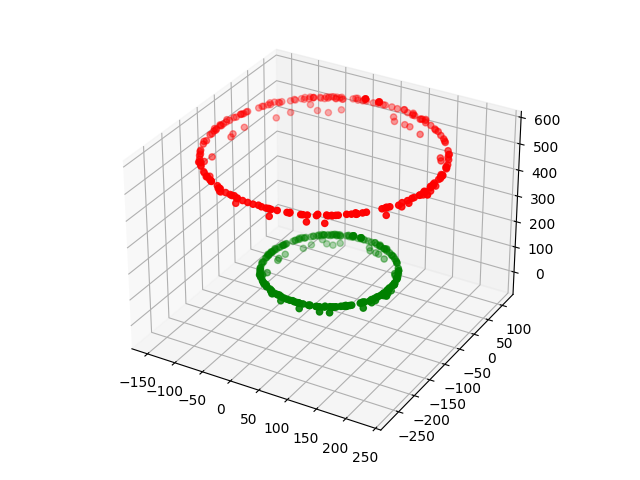
\includegraphics[width=0.7\linewidth]{images/electronic/mycalibration.png}
	\caption{Results of the calibration with the sensor used in the project. The red dots are the original readings, the green are the compensated values.\\}
\end{figure}

\newpage	
\section{Software}\label{sec:software}
This section is dedicated to explain the software architecture and show some implementation details. 

There are two components: a \texttt{systemd} service that starts the main software, and the core of the software, written in Python. 

The \textbf{main software} is composed of 5 files: 
\begin{enumerate}
	\item \texttt{main.py}: in this file, the values of the sensors (button, gps, ...) are read and the actuators (the motors) are used accordingly
\end{enumerate}

The other 4 files are auxiliary files, inside the folder \texttt{lib}:

\begin{enumerate}
	\setcounter{enumi}{1}
	\item \texttt{motors.py}: contains the functions to run the motors;
	\item \texttt{gps.py}: contains the function to receive and parse data from the gps sensor;
	\item \texttt{compass.py}: reads the magnetometer data and computes the angle between the current heading and the north;
	\item \texttt{accel.py}: reads the data from the accelerometer positioned on the \textit{top} plane to check its tilting angle. 
\end{enumerate}

The use of the star tracker is fairly simple: first of all, it needs to receive its gps location and its orientation, after which the button can be pressed by the user to start the plane tilting and at last the actual tracking. But these operation do not need to be run sequentially, and for some it is actually impossible: the user can press the button at any time, so they should be run with some form of concurrency, that allow the star tracker to perform its operations while listening for user input. 

The adopted solution is to use the \textbf{asynchronous} paradigm, made possible in Python by the relatively new \texttt{asyncio} module and \texttt{async/await} keywords. This paradigm is particularly suitable for this use case, since it is dominated by various I/O operations rather than cpu-bound ones, where instead threading programming is better \cite{asyncpython}. In this paradigm a single thread is used, where different \textit{coroutines} are executed concurrently: the coroutines are a central idea of this design, and can be considered as functions that are able to be paused and resumed later. In a typical execution, then, there are different coroutines, and only one is running at a time: when the running coroutine has nothing to do, because e.g. it's waiting an output operation to finish, it can suspend its execution and another will be resumed.

\subsection{\texttt{main.py}}

After having introduced the paradigm used, \texttt{main.py} will be analysed in more detail. This file has 5 tasks, as the listing \ref{lst:maintasks} shows:

\begin{lstlisting}[language=PythonPlus, label={lst:maintasks}, caption=main tasks]
async def main():
  task_button = asyncio.create_task(listen_button()) 
  task_gps_compass = asyncio.create_task(listen_gps_compass())
  task_tracking = asyncio.create_task(tracking())
  task_accel = asyncio.create_task(listen_accel())
  task_led = asyncio.create_task(control_led())
  await asyncio.gather(task_button, task_gps_compass, task_tracking, task_accel, task_led) 
\end{lstlisting}


These tasks wait for some conditions to be met; for example, \texttt{task\_led} turns on the led when the star tracker is correctly oriented towards north. To know when the conditions are met, every task checks some global variables, show in listing \ref{lst:globvar}; if they are \texttt{False/None/empty}, the tasks pauses for 1 second. \texttt{task\_button}, \texttt{task\_tracking} and \texttt{task\_led} run forever, while \texttt{task\_gps\_compass} and \texttt{task\_accel} return after their job is done. 


\begin{lstlisting}[language=PythonPlus, label={lst:globvar}, caption=Global variables used to coordinate the tasks]
is_running = False      # status of the star tracker (running/not running)
is_ready_1 = False      # wether the star tracker points to north and we have gps data
is_ready_2 = False      # wether the star tracker is ready to track (in the correct position)
\end{lstlisting}

Figure \ref{fig:mainsequence} shows the "interaction", or to be more precise, the coroutines running during a typical flow of execution.

\begin{figure}[h]
	\centering
	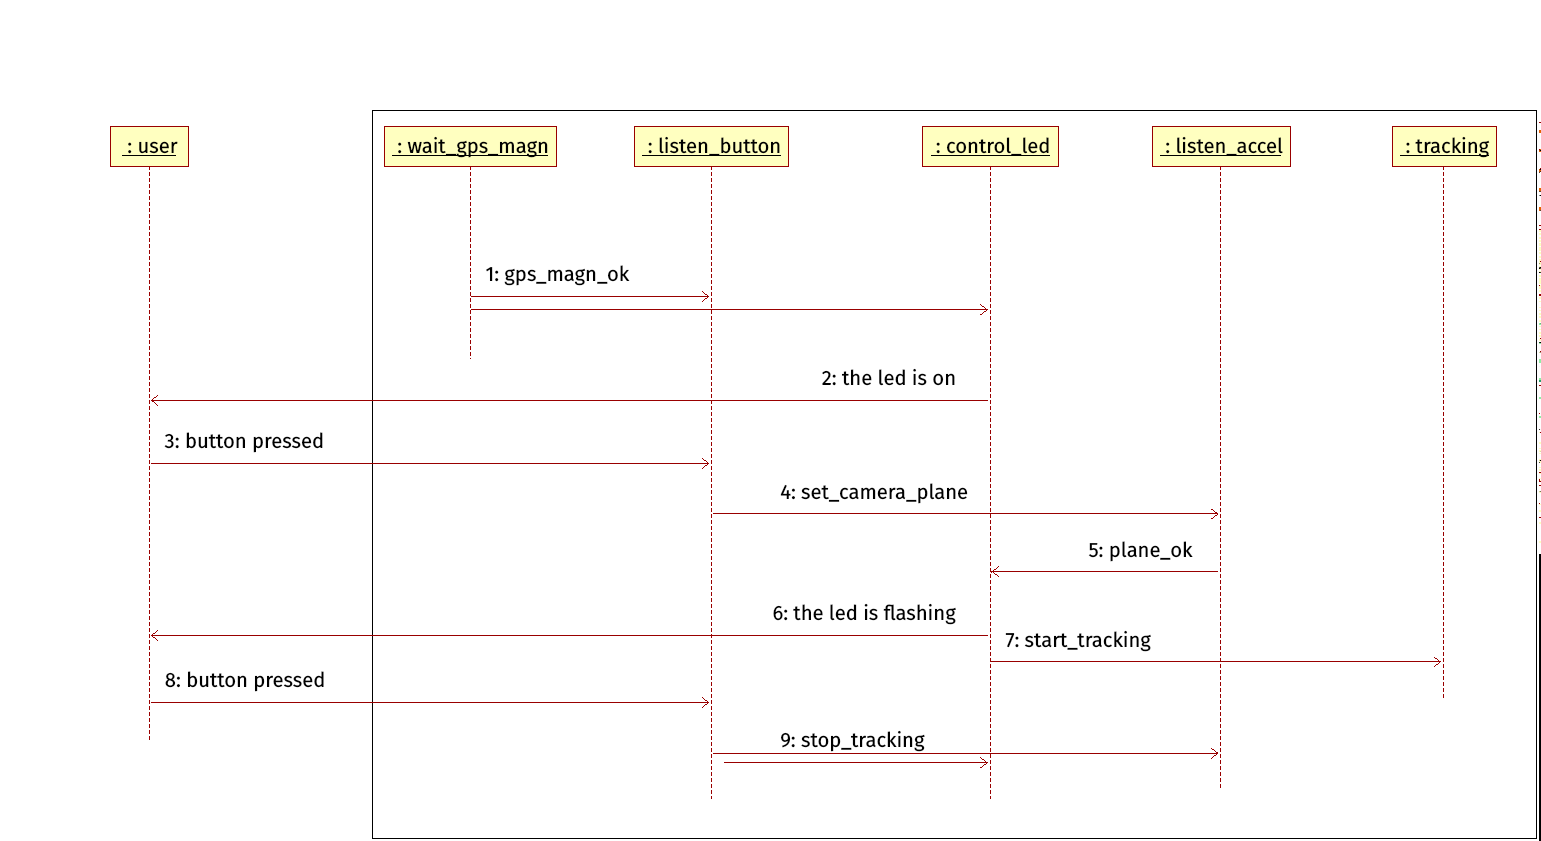
\includegraphics[width=\linewidth]{images/software/main_sequence.png}
	\caption{Typical flow of execution. The objects are the coroutines.}
	\label{fig:mainsequence}
\end{figure}

In the following paragraphs is explained what the coroutines do.

\paragraph{wait\_gps\_magn} This coroutine, which is actually called \texttt{listen\_gps\_compass} but shortened in \ref{fig:mainsequence}, listens for the gps signal; after having received the location and the current date, these information can be used to point the star tracker towards north: in fact, the actual geographic north is shifted from the magnetic north, and this phenomenon is called \textit{declination} (see section \ref{sec:mag_decl}). This depends on the location and date. The library \texttt{wmm2020} \cite{wmm2020} is used to compute the declination angle.

\begin{lstlisting}[mathescape, language=PythonPlus, label={lst:waitgps}, caption=Extract from the \texttt{listen\_gps\_compass} coroutine: it makes the base motor vibrate according to the actual heading.]
if  _compass < 180: #we are, e.g., at 40${^\circ}$ from north and must turn anticlockwise
	print("we should turn a bit anticlockwise, vibrate once for", _compass/90, "seconds")
	# let's signal it to the user with a vibrations:
	motors.vibrate("z", _compass/90) #vibration in seconds: 180 = 2 sec, 90 = 1 sec etc.
	
	time.sleep(3) #time for the user to make the adjustement
else: #we are, e.g. 330${^\circ}$ = 30${^\circ}$ from north and must turn clockwise
	print("we should turn a bit clockwise, vibrate twice for", _compass/180, "seconds each")
	# let's signal it to the user with two vibrations:
	motors.vibrate("z", (360 - _compass)/180) #it's like (_compass/90)/2
	time.sleep(0.5)
	motors.vibrate("z", (360 - _compass)/180) #it's like (_compass/90)/2
	
	time.sleep(3) #time for the user to make the adjustement
\end{lstlisting}

The motor inside the \textit{base} vibrates according to how many degrees the rest of the star tracker needs to rotate: if it needs to rotate anticlockwise, the duration in seconds is given from $\frac{\textnormal{actual heading}}{90}$: the maximum duration is 2 seconds when the actual heading is $180^\circ$, and decreases as the angle gets close to 0. 

If the actual heading is greater than $180^\circ$, and the rotation can be done clockwise, it is signalled through the same mechanism, but with two vibration, which duration is computed through the same mechanism and divided by two; so the maximum of each vibration is 1 second. 

The user has then some time to make the adjustments.

This coroutine sets the variable \texttt{is\_ready\_one}. 

Note that the position given from the gps and the angle given from the magnetometer are read multiple times and averaged.

\paragraph{listen\_button} This coroutine listens for button input by the user. If the global variable \texttt{is\_ready\_1} is true, a button press above 3 seconds will set \texttt{is\_running} to true, otherwise to false. If the pressing lasts more than 10 seconds, the Raspberry will shut down.
\paragraph{control\_led} This coroutine checks the global variables \texttt{is\_ready\_one} and \texttt{is\_ready\_two} to know at which state the star tracker is. If both are false, the led is turned off; if the first one is true, the led is turned on; if both are true, it first blinks sequentially faster, and each blink duration derives from the Fibonacci's sequence: $\sum_{i=1}^{12}\frac{1}{fib(i)}$, which gives the user around 9 seconds to press the shutter button on the camera; and then blinks twice every 30 seconds, to signal that the tracking is in progress. 
\paragraph{listen\_accel} This coroutine waits until the global variables \texttt{is\_ready\_one} \texttt{is\_running} are true; then, after reading the tilt of the \textit{top} plane from the accelerometer installed there, runs the motor for the necessary steps and waits 15 seconds before reading the value again. This is done because the user may want to change the camera position after installing it, altering the tilt. If two consecutive reads report the correct value, the variable \texttt{is\_ready\_two} is set to true.

As in the gps/magnetometer case, the values are read multiple times and averaged. 

The number of steps necessary to move in the correct position depends on the gear ratio and the stepping angle, which is $1.8^\circ$, as shown in listing \ref{lst:steps}. The target angle is given from the latitude, in turn obtained from the gps. 

\begin{lstlisting}[language=PythonPlus, label={lst:steps}, caption=The computation inside \texttt{listen\_accel} to compute the steps needed to move in the correct position the \textit{top} plane.]
distance = gps_data[0] - _tilt # tilt is the actual tilt - from the averaged readings
# ...
rot2  = distance*gear_ratio2
step1 = abs(int((rot2*gear_ratio1)/1.8))
print("accel: we are at tilt", _tilt, "and need to go to", gps_data[0])
print("accel:", step1, "steps needed to position correctly - distance is", distance)
if distance > 0:
	print("accel: I need to move clockwise")
	motors.move("x", step1, clockwise=True)
else:
	print("accel: I need to move anticlockwise")
	motors.move("x", step1, clockwise=False)
\end{lstlisting}

\paragraph{tracking} This coroutine checks the variable \texttt{is\_ready\_two} and, when it is true, runs the bigger motor to move the camera. Before running, it waits 10 seconds, during which concurrently the led is flashing to alert the user. 
\\
\\
In the following subsections, the other files will be analysed. 

\begin{figure}[h]
	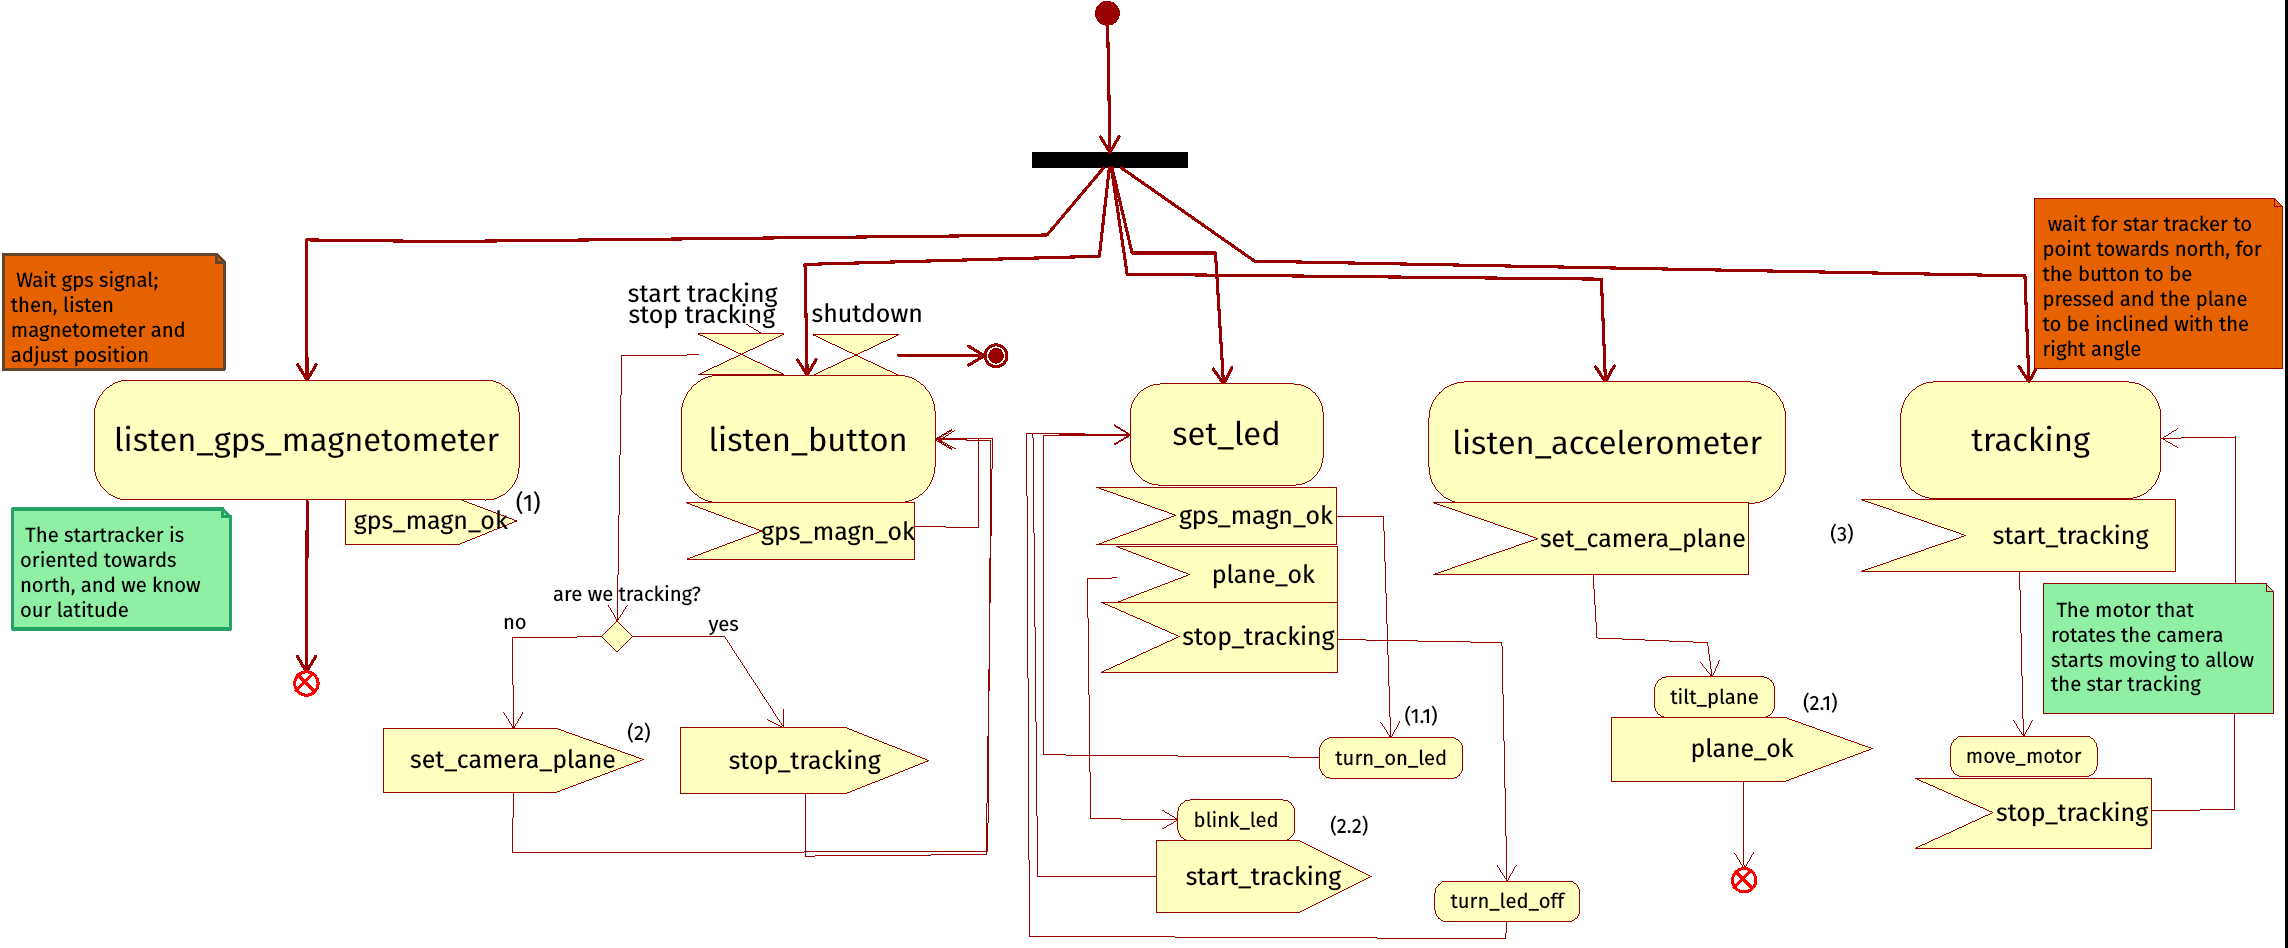
\includegraphics[width=\linewidth]{images/software/main_activity_diagram.png}
	\caption{The activity diagram for \texttt{main.py}: \textbf{1.} the star tracker receives the gps position and is headed towards north; \textbf{1.1.} the led is turned on to nofify the user; \textbf{2.} the user presses the button, \textbf{2.1.} the \textit{top} plane is tilted and \textbf{2.2.} and the led starts blinking; \textbf{3.} after a timeout, during which the led blinks, the biggest motor starts moving to allow the actual tracking.}
\end{figure}

\subsection{\texttt{motors.py}}
This file is responsible for the movement of the motors. They are identified with three letters: \texttt{x} for the one on the \textit{middle} part, \texttt{y} identifies the one in the \textit{top} plane and \texttt{z} is for the one \textit{base} part. The letters refer to the axis on with the rotation occurs.

Since these motors are stepper motors, it is possible to move them when the right sequence of signal is sent to their driver. They are hence driven using Raspberry's GPIO, which are set to output a signal or not output a signal, as shown in listing \ref{lst:motmove}: the motors have two coils, when the current passes in one direction in one coil, it creates a magnetic field; when the current passes in the same coil in the other direction, the magnetic filed is inverted. This makes the stator move. So, the variable \texttt{step\_sequence} contains the list of pins that need to output the signal (can be more than one at a time) for a step to occur. 

\begin{lstlisting}[language=PythonPlus, label={lst:motmove}, caption=The main code for the function \texttt{move} in \texttt{motors.py}.]
def move(motor, steps, clockwise=True):
	# ...
	while True:
	for pin_list in step_sequence:
		for pin in pins:
			if pin not in pin_list:
				GPIO.output(pin, True)
			else:
				GPIO.output(pin, False)
			steps -= 1
			if steps < 0:
				return
			print("steps remaining in move:", steps, end="\r")
			time.sleep(WAIT)
\end{lstlisting}

A global variable, \texttt{motor\_pins}, specifies which pins control which motor, and in what order they must be used. Then, according to how the motor needs to be driven, a step sequence is generated, as shown in listing \ref{lst:stepsequence}:

\begin{lstlisting}[language=PythonPlus, label={lst:stepsequence}, caption=Generation of a step sequence to move a motor inside the \texttt{move} function.]

step_sequence = list(range(4))

pins = copy.deepcopy(motor_pins[motor]) # this is equal to e.g. [1,2,3,4]

if not clockwise:
	pins.reverse()

step_sequence[0] = [pins[0], pins[1]]
step_sequence[1] = [pins[1], pins[2]]
step_sequence[2] = [pins[2], pins[3]]
step_sequence[3] = [pins[0], pins[3]]

\end{lstlisting}

There are three main functions in this file. 

\paragraph{lock\_motor} Set the first two pins of the given motor to true, and the other to false. This has the effect of "locking" the motor in place.

\paragraph{move} This function is shown in the above listings, \ref{lst:motmove} and \ref{lst:stepsequence}. It can move a given motor for a given number of steps; there is another input variable to specify if the movement should be clockwise or counter-clockwise. 

\paragraph{move\_microstep} This function is a variant of the \texttt{move} function. The idea behind it is, instead of setting the output in a binary fashion (signal or not signal), use the \textbf{pulse width modulation} technique, which allows to simulate an analog signal. This makes the rotation smoother, in \textbf{microstep}, instead of normal $1.8^\circ$ steps. This is done to allow a longer time to complete a rotation, since a really slow rotation is needed to allow the star tracking. 

The duration of a step is computed considering the step sequence, which is longer than the \texttt{move} one, the ratio between the gears and the \textbf{sidereal day} duration in seconds, which is the total time during which the complete rotation must take place. Listing \ref{lst:sidcomput} shows it. 

\begin{lstlisting}[language=PythonPlus, label={lst:sidcomput}, caption={\texttt{move\_microstep} function, showing the computations for how much time wait between a step and another.}]
wait_between_steps = (sidereal_day/(200*4*gear_ratio)) - wait_time #here 50 comes from 200/4
\end{lstlisting}

200 is the number of steps to make a rotation (since each step is $1.8^\circ \Rightarrow 1.8*50=360$), 4 is the number of microsteps (technically every step is composed of 2 microsteps, but since the step sequence is longer, 400 steps are needed). This gives a wait time of about 14 seconds.

If $A$ is coil in which the current flows in a certain direction and $\bar{A}$ is when the current flows in the opposite direction, and the same goes for the other coil $B$, then the step sequence is given from $AB > B > \bar{A}B > \bar{A} > \overline{AB} > \bar{B} > A\bar{B} > A$. 

To conclude, \ref{lst:pwm} shows another snippet of code from the function $move\_microstep$, that shows how the pwm is implemented:

\begin{lstlisting}[language=PythonPlus, label={lst:pwm}, caption=The use of the pwm capability of the Raspberry in the \texttt{move\_microstep} function.]
async def move_microstep(motor, steps, sleep=False, clockwise=True):
	# ...
	wait_between_steps = (sidereal_day/(200*4*gear_ratio)) - wait_time 

	pin_pwm_1 = GPIO.PWM(pins[0],frequency)		#create PWM instance with frequency
	# ...
	pin_pwm_1.start(0)				#start PWM of required Duty Cycle 
	pin_pwm_2.start(0)				#start PWM of required Duty Cycle 
	pin_pwm_3.start(0)				#start PWM of required Duty Cycle 
	pin_pwm_4.start(0)				#start PWM of required Duty Cycle 

	first_time=True
	while True:
		for duty in range(0, max_pwm_value+1, resolution):
		
			pin_pwm_1.ChangeDutyCycle(duty)
			time.sleep(wait_time)
			if sleep:
				await asyncio.sleep(wait_between_steps)
		# ...
		
\end{lstlisting}

\subsection{\texttt{gps.py}}
This file is responsible for handling the gps module. Since the communication with this chip happens through the serial protocol, to get data from the gps this communication must be initialized. The data is then parsed through a library, \texttt{pynmea2}. This is because gps send data in the \textit{NMEA} standard \cite{gps_nmea}. 

The listing \ref{lst:gps} shows the important parts of the code.

\begin{lstlisting}[language=PythonPlus, label={lst:gps}, caption=Code for the \texttt{gps.py} file. The serial port initialization and data parsing are shown.]
def _port_setup(port):
	ser = serial.Serial(port, baudrate=9600, timeout=2)
	return ser

def _parseGPSdata(ser):
	keywords = ["$GPRMC","$GPGGA"]
	gps_data = ser.readline()
	gps_data = gps_data.decode("utf-8")  # transform data into plain string
	try:
		nmeaobj = pynmea2.parse(gps_data)
	except Exception as e:
		print(e)

	if len(gps_data) > 5:  # Check to see if the GPS gave any useful data
		if gps_data[0:6] in keywords:   # Check t see if the message code
			try:
				gps_msg = pynmea2.parse(gps_data)
				lat = gps_msg.latitude
				lng = gps_msg.longitude
				alt = gps_msg.altitude 
				date = gps_msg.timestamp
				return (lat,lng,alt,date)
			except:
				return None
	return None
\end{lstlisting}

\subsection{\texttt{compass.py}}

\begin{floatingfigure}[r]{0.35\linewidth}
	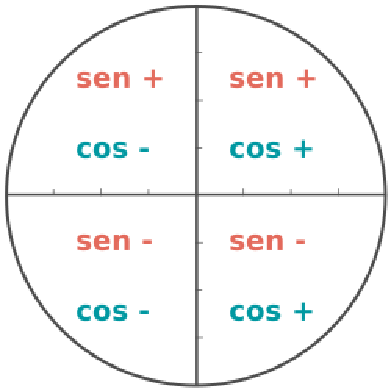
\includegraphics[width=0.33\linewidth]{images/software/signe}
	\caption{arcsine and arccosine cannot tell the difference between some angles, e.g. the arcsine for $x$ and $x+90^\circ$ is the same.\\}
\end{floatingfigure}

This file is responsible for the communication with the magnetometer sensor. Since it is an Adafruit product, there is a fairly easy to use library, \texttt{adafruit\_icm20x}, which handles all the communication. The data can be obtained simply calling the \texttt{icm.magnetic} member of the class \texttt{ICM20948}, which stores the magnetic field along the x, y and z axis: \texttt{mx, my, mz}. 

Then, this data is used to correct for hard and soft iron disturbances, as explained in section \ref{sec:iron_calib}. 

After the data is adjusted, the heading can be calculated as the arctangent between the y and x component: this is because while the the heading can be at any angle, (arc)sine and (arc)cosine can only determine if this angle is in the first or fourth quadrant, and in the first and second quadrant, respectively; \texttt{atan2(y, x)} considers instead the signs of x and y and can determine any angle. 

The process is showed in listing \ref{lst:magcal}.

\begin{lstlisting}[language=PythonPlus, label={lst:magcal}, caption={The magnetic field is read from the sensor, the calibration parameters are applied and the heading is computed.}]
def get_position():
	mx, my, mz = icm.magnetic

	corrected_xyz = np.dot(si, np.array([mx - hi[0], my - hi[1], mz - hi[2]]))
	
	heading_rad = atan2(corrected_xyz[1], corrected_xyz[0])
	
	if (heading_rad < 0):
		heading_rad += 2*np.pi
	
	if (heading_rad > 2*np.pi):
		heading_rad -= 2*np.pi
	
	heading = np.rad2deg(heading_rad)
	
\end{lstlisting}

\subsection{\texttt{accel.py}}
The accelerometer sensor uses the \texttt{i2c} communication protocol. Since the Raspberry has a physical bus that was already in use by the magnetometer, 
a software one was defined, as explained in \ref{sec:communication}.

In this case no library was used; the process to compute the tilt angle is roughly the same explained for the magnetometer, i.e. the arctan is considered between y and the hypotenuse between x and z. But there is also a slight more complicated setup process. 

To begin with, the bus is defined at the i2c port 11, and the device address is \texttt{0x68}; then the register \texttt{PWR\_MGMT\_1} is set. This register allows the user to configure the power mode and clock source \cite{sparkfun}.

\begin{lstlisting}[language=PythonPlus, caption=Sensor initialization.]
power_mgmt_1 = 0x6b
power_mgmt_2 = 0x6c

bus = smbus.SMBus(11)
address = 0x68       
	
# ...
	
def _init() :
	bus.write_byte_data(address, power_mgmt_1, 0)
	
\end{lstlisting}

Individual byte are read, composed into words and scaled accordingly to their value from the appropriate registers:

\begin{lstlisting}[language=PythonPlus, caption=A word is a two byte value read from a register.]
def read_byte(adr):
	return bus.read_byte_data(address, adr)

def read_word(adr):
	high = bus.read_byte_data(address, adr)
	low = bus.read_byte_data(address, adr+1)
	val = (high << 8) + low
	return val

def read_word_2c(adr):
	val = read_word(adr)
	if (val >= 0x8000):
		return -((65535 - val) + 1)
	else:
		return val
\end{lstlisting}

Since the registers have 16 bits, the maximum value read is $2^{16} = 65536$; to get signed values, if the value is more or equal than half of $2^{16}$, which means $2^8$ (in hexadecimal is \texttt{0x8000}), the negative value is returned. 

Finally, the value read will be divided by 16384, which is the maximum value that can be read at the default sensitivity, to scale it. 

\section{Results}
In this section, the results of the implementation are briefly discussed, and then commented more deeply in the conclusion. 

To begin with, some \textbf{hard constrains} are summarized:

\begin{itemize}
	\item since the wait time between steps is around 14 seconds, the maximum focal length allowed is around 18mm, otherwise the star trail will start to appear;
	\item due to dimensions of the motor and gear ratio, only cameras below 1 kg of weight can be used, and its centre of mass should be the nearest possible to the axis of rotation; in other words, cameras with too long lens could cause the motor to stall;
	\item the battery cannot run for too long, only 2 shoot with 5 mins of exposure each should be possible. 
\end{itemize}

With that being said, here are examples of actual photos taken with the star tracker \ref{fig:startrackerresult}:

\begin{figure}[H]
	\centering
	\subfigure[Exposure: 306 seconds, focal length: 18mm, aperture: f/10. Shoot with Nikon D3300. ]{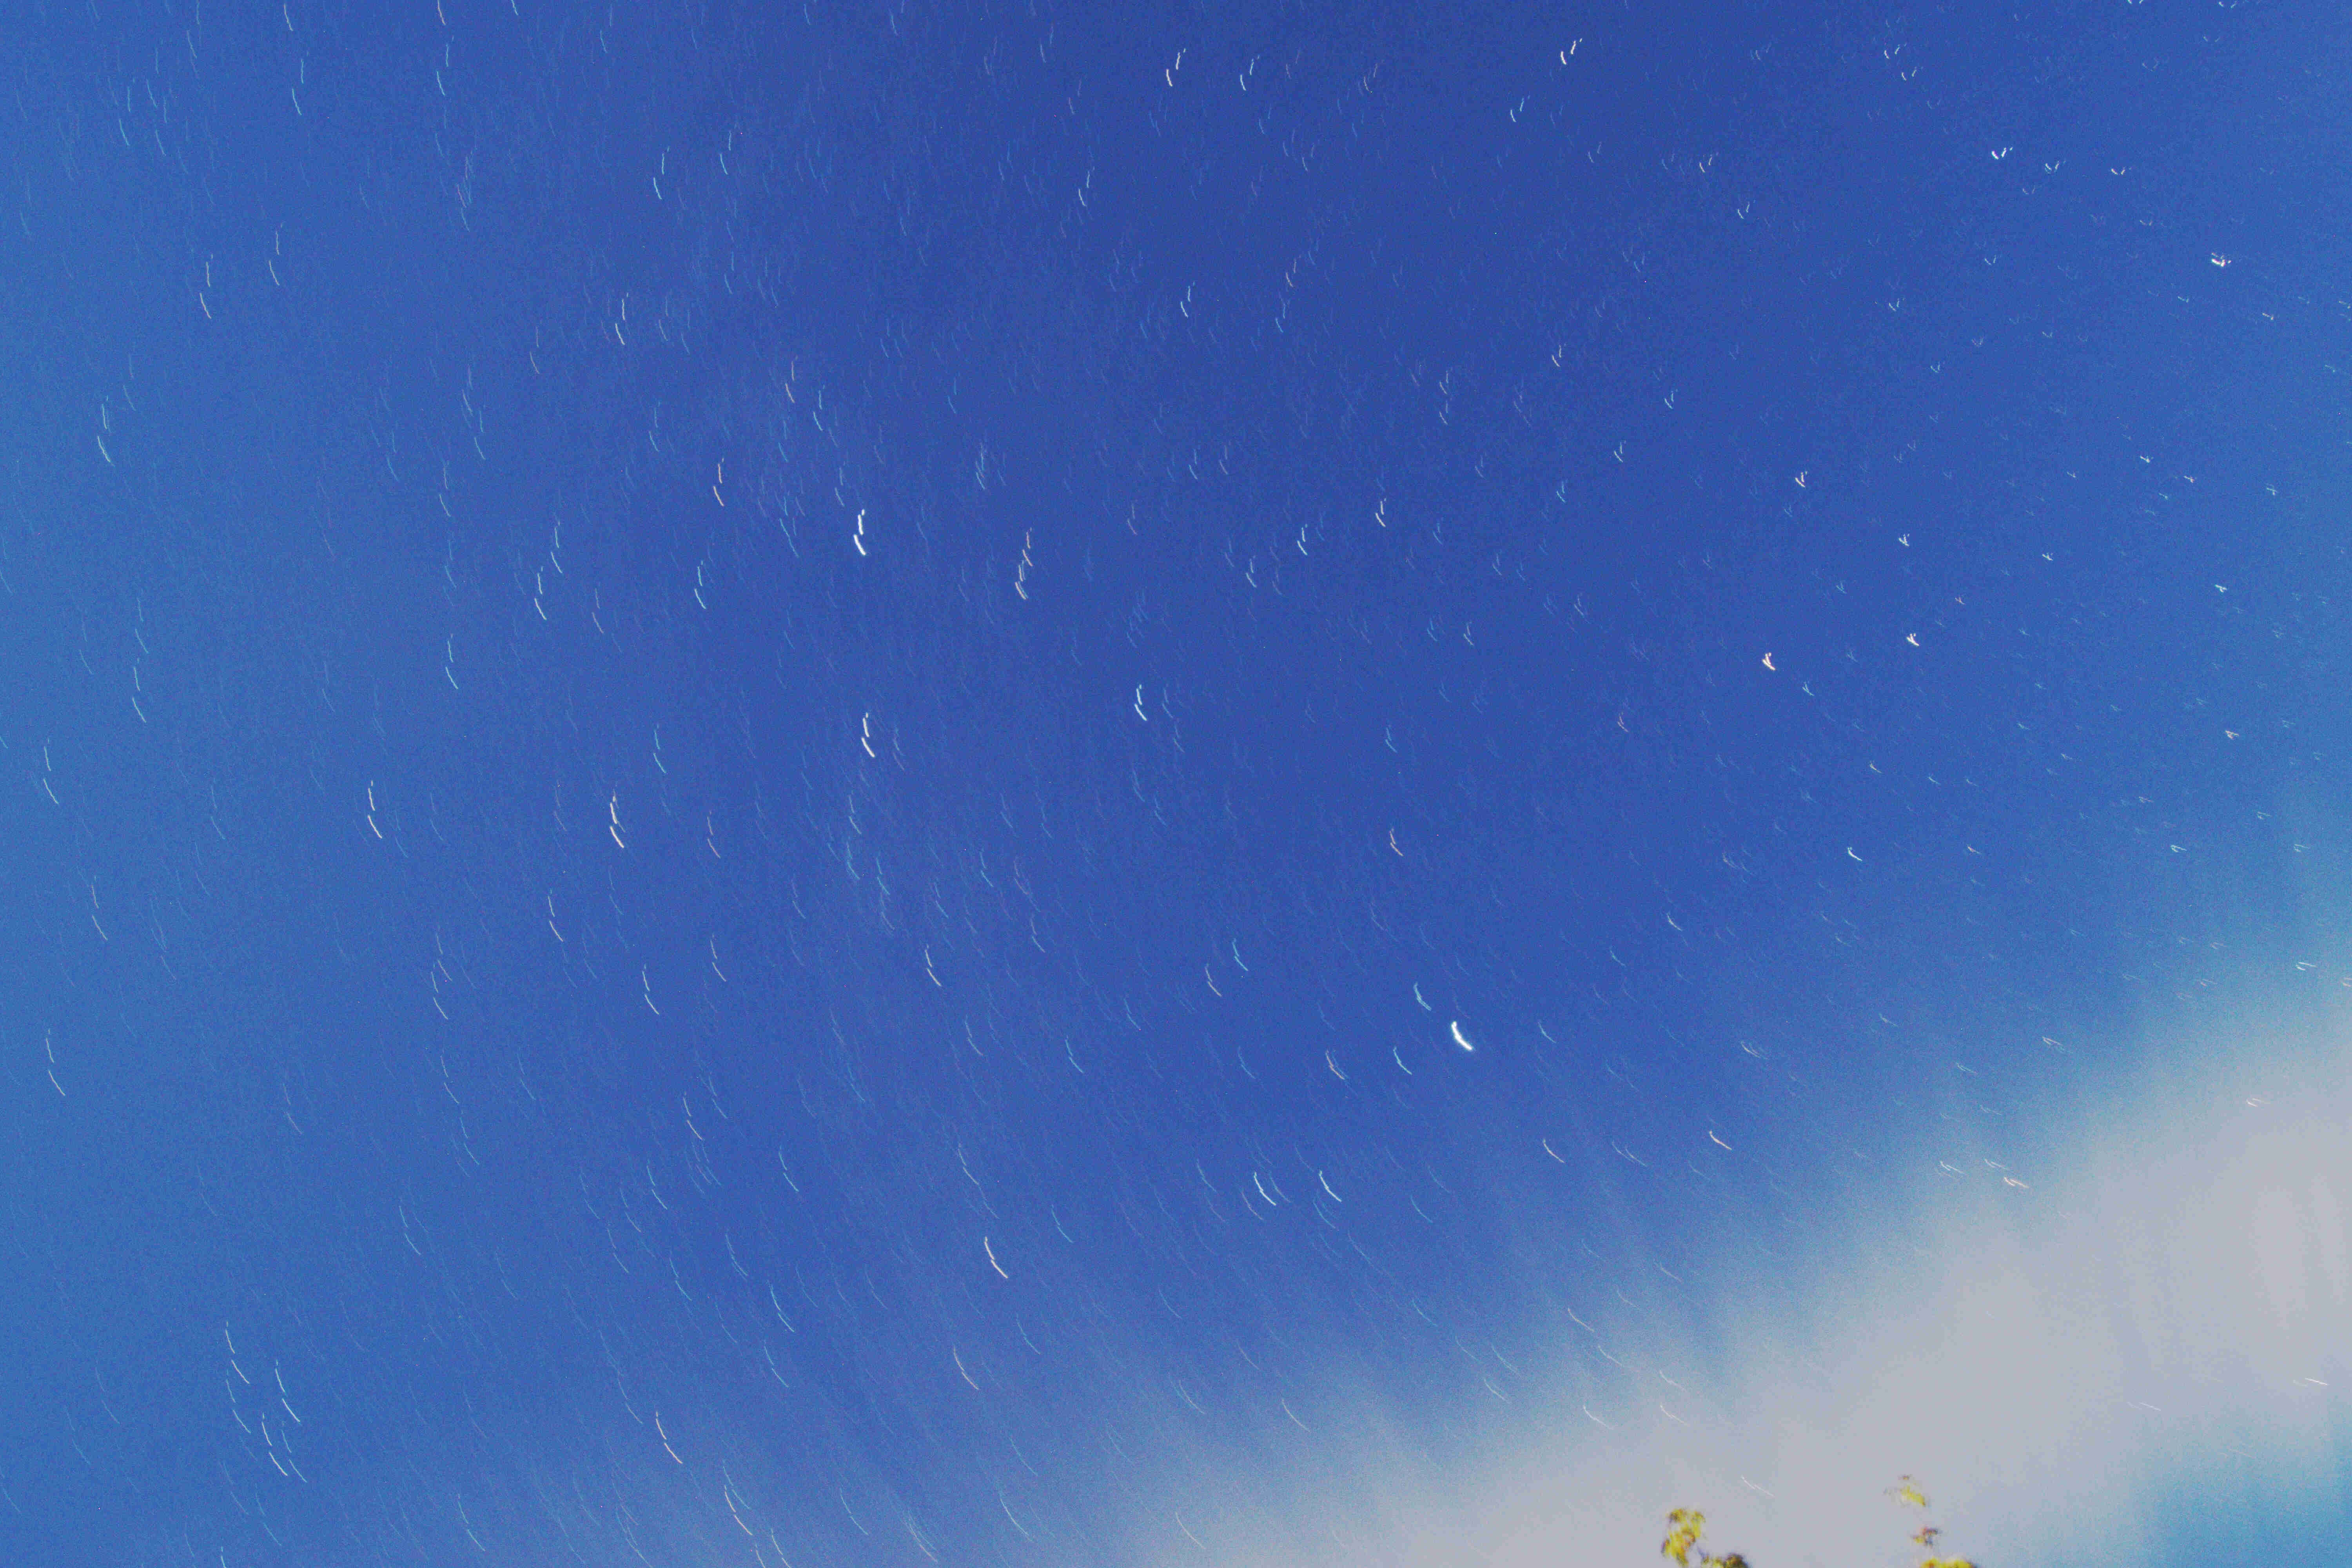
\includegraphics[width=0.45\linewidth, clip, trim=300 400 500 200 ]{images/results/DSC_2296}}
	\subfigure[Exposure: 399 seconds, focal length: 18mm, aperture: f/14. Shoot with Nikon D3300.]{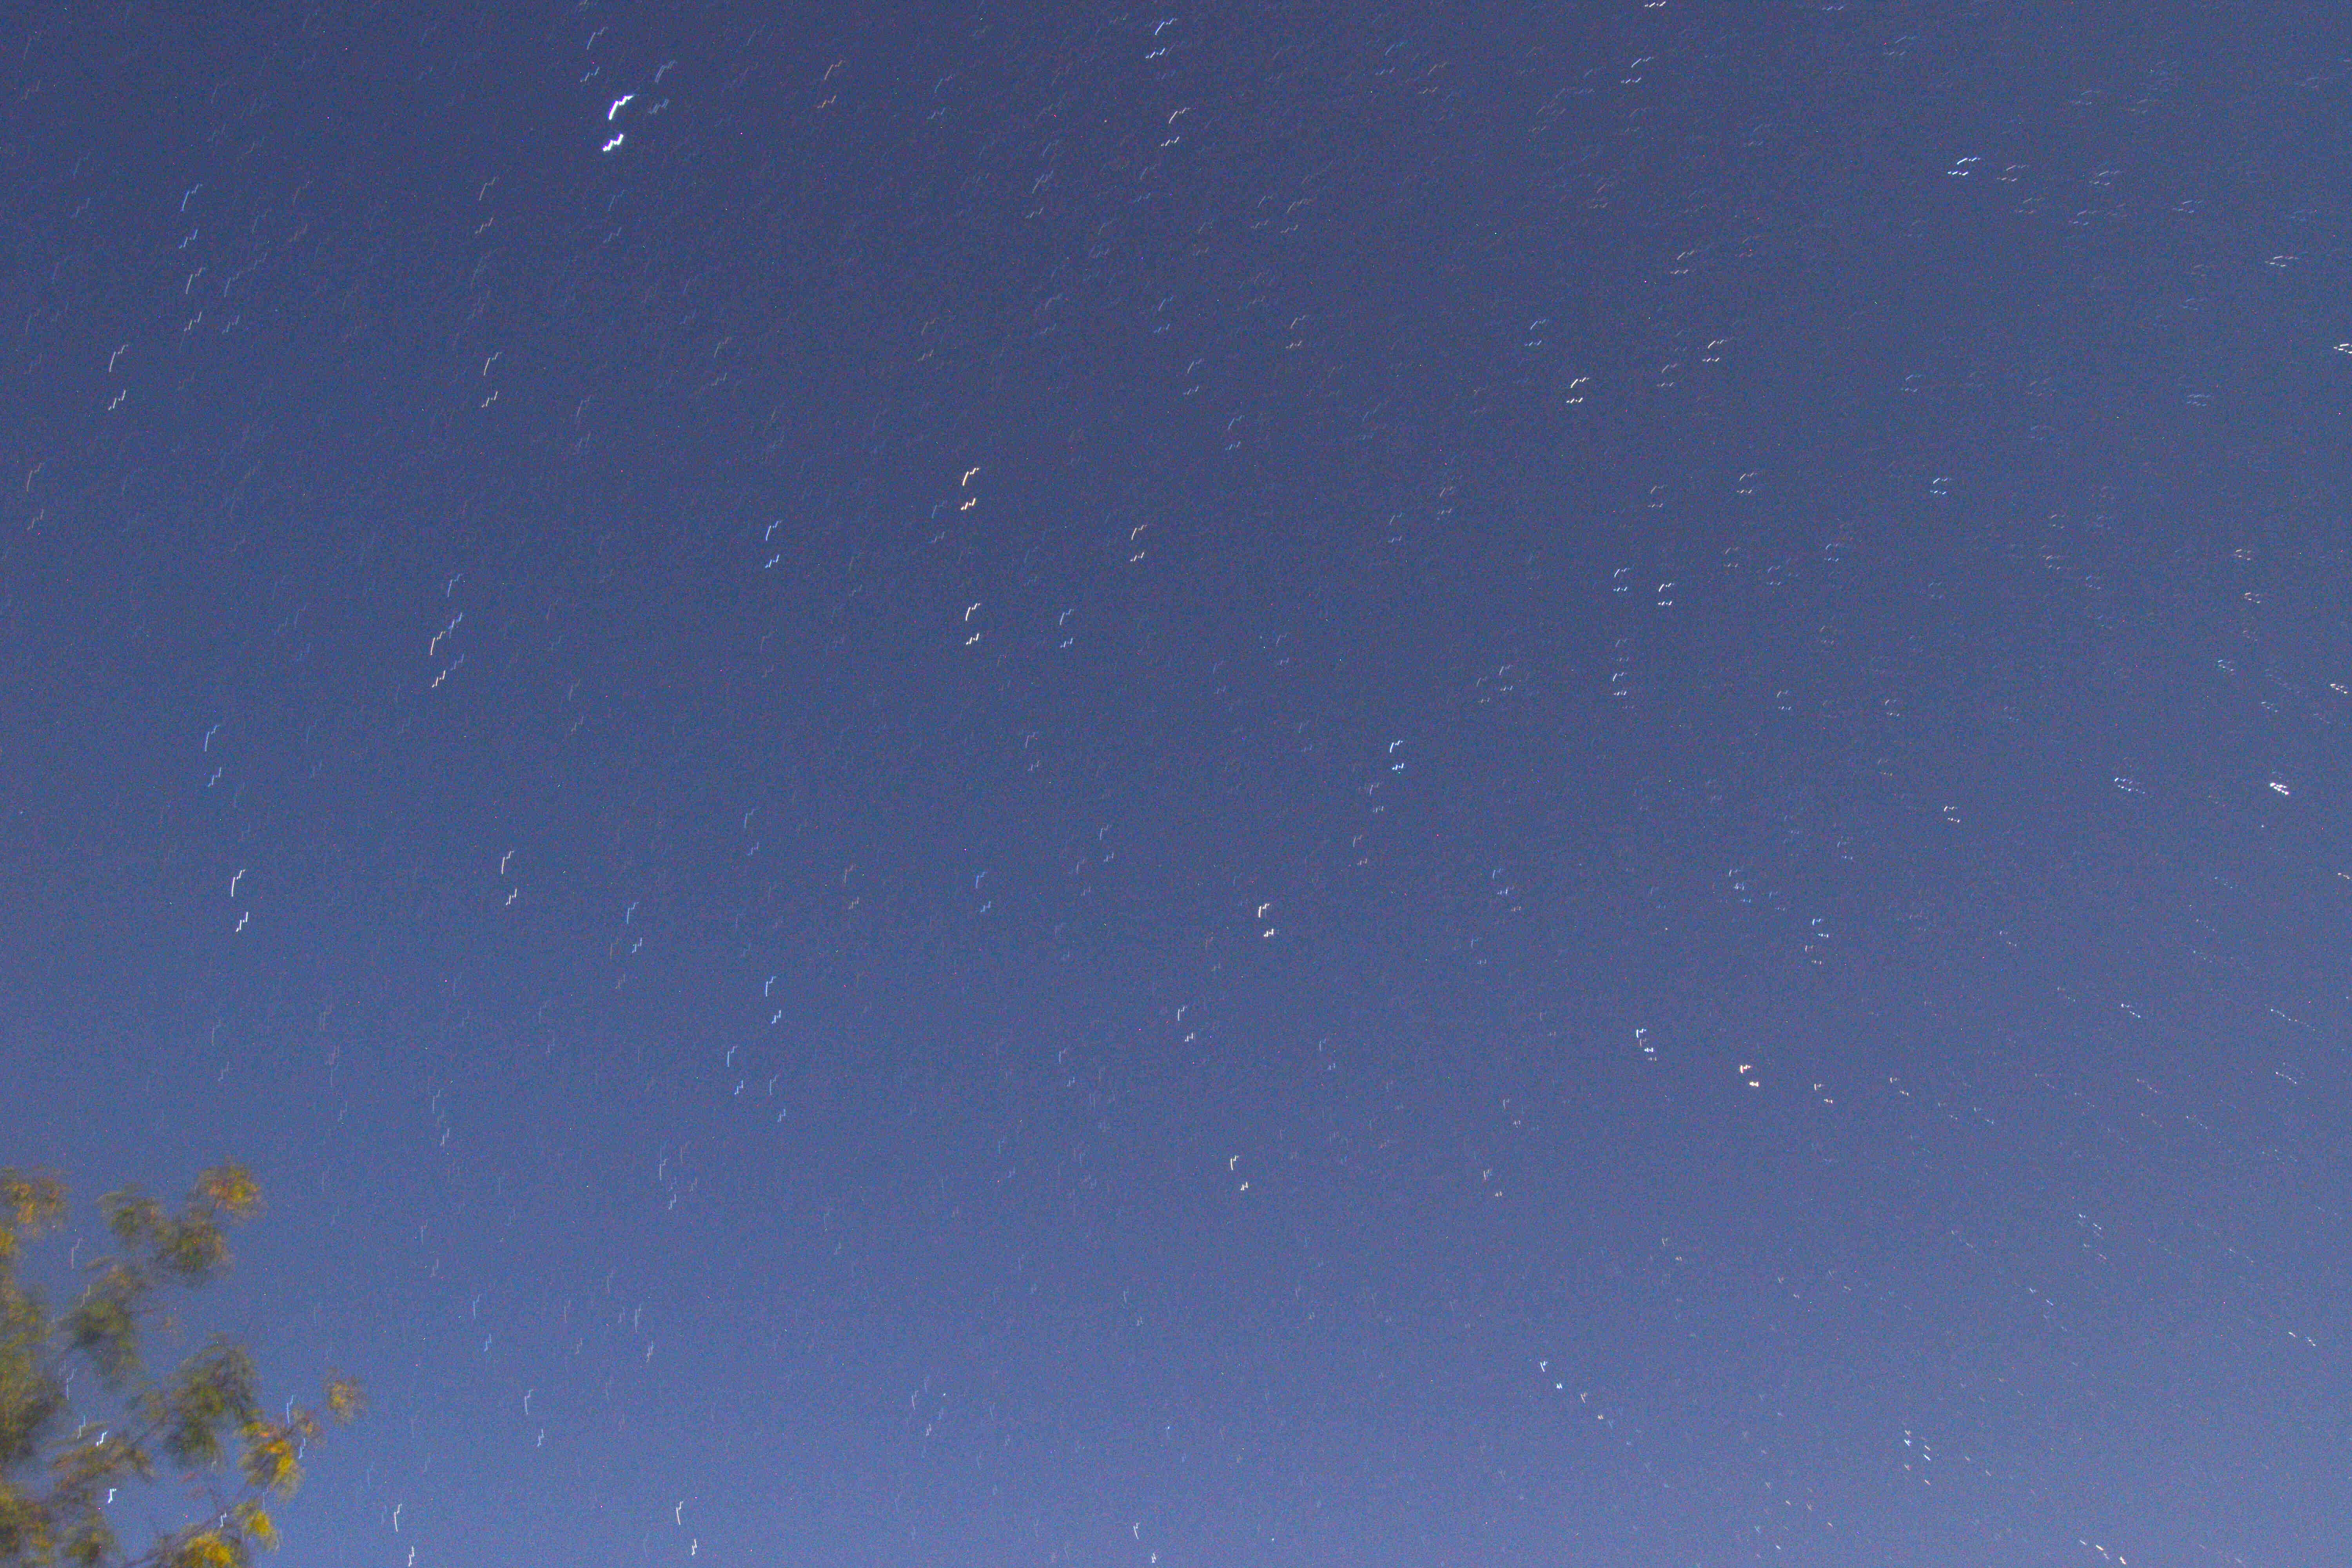
\includegraphics[width=0.45\linewidth, clip, trim=200 600 600 0 ]{images/results/DSC_2300}}
	\subfigure[Exposure: 645 seconds, focal length: 18mm, aperture: f/14. Shoot with Nikon D3300.]{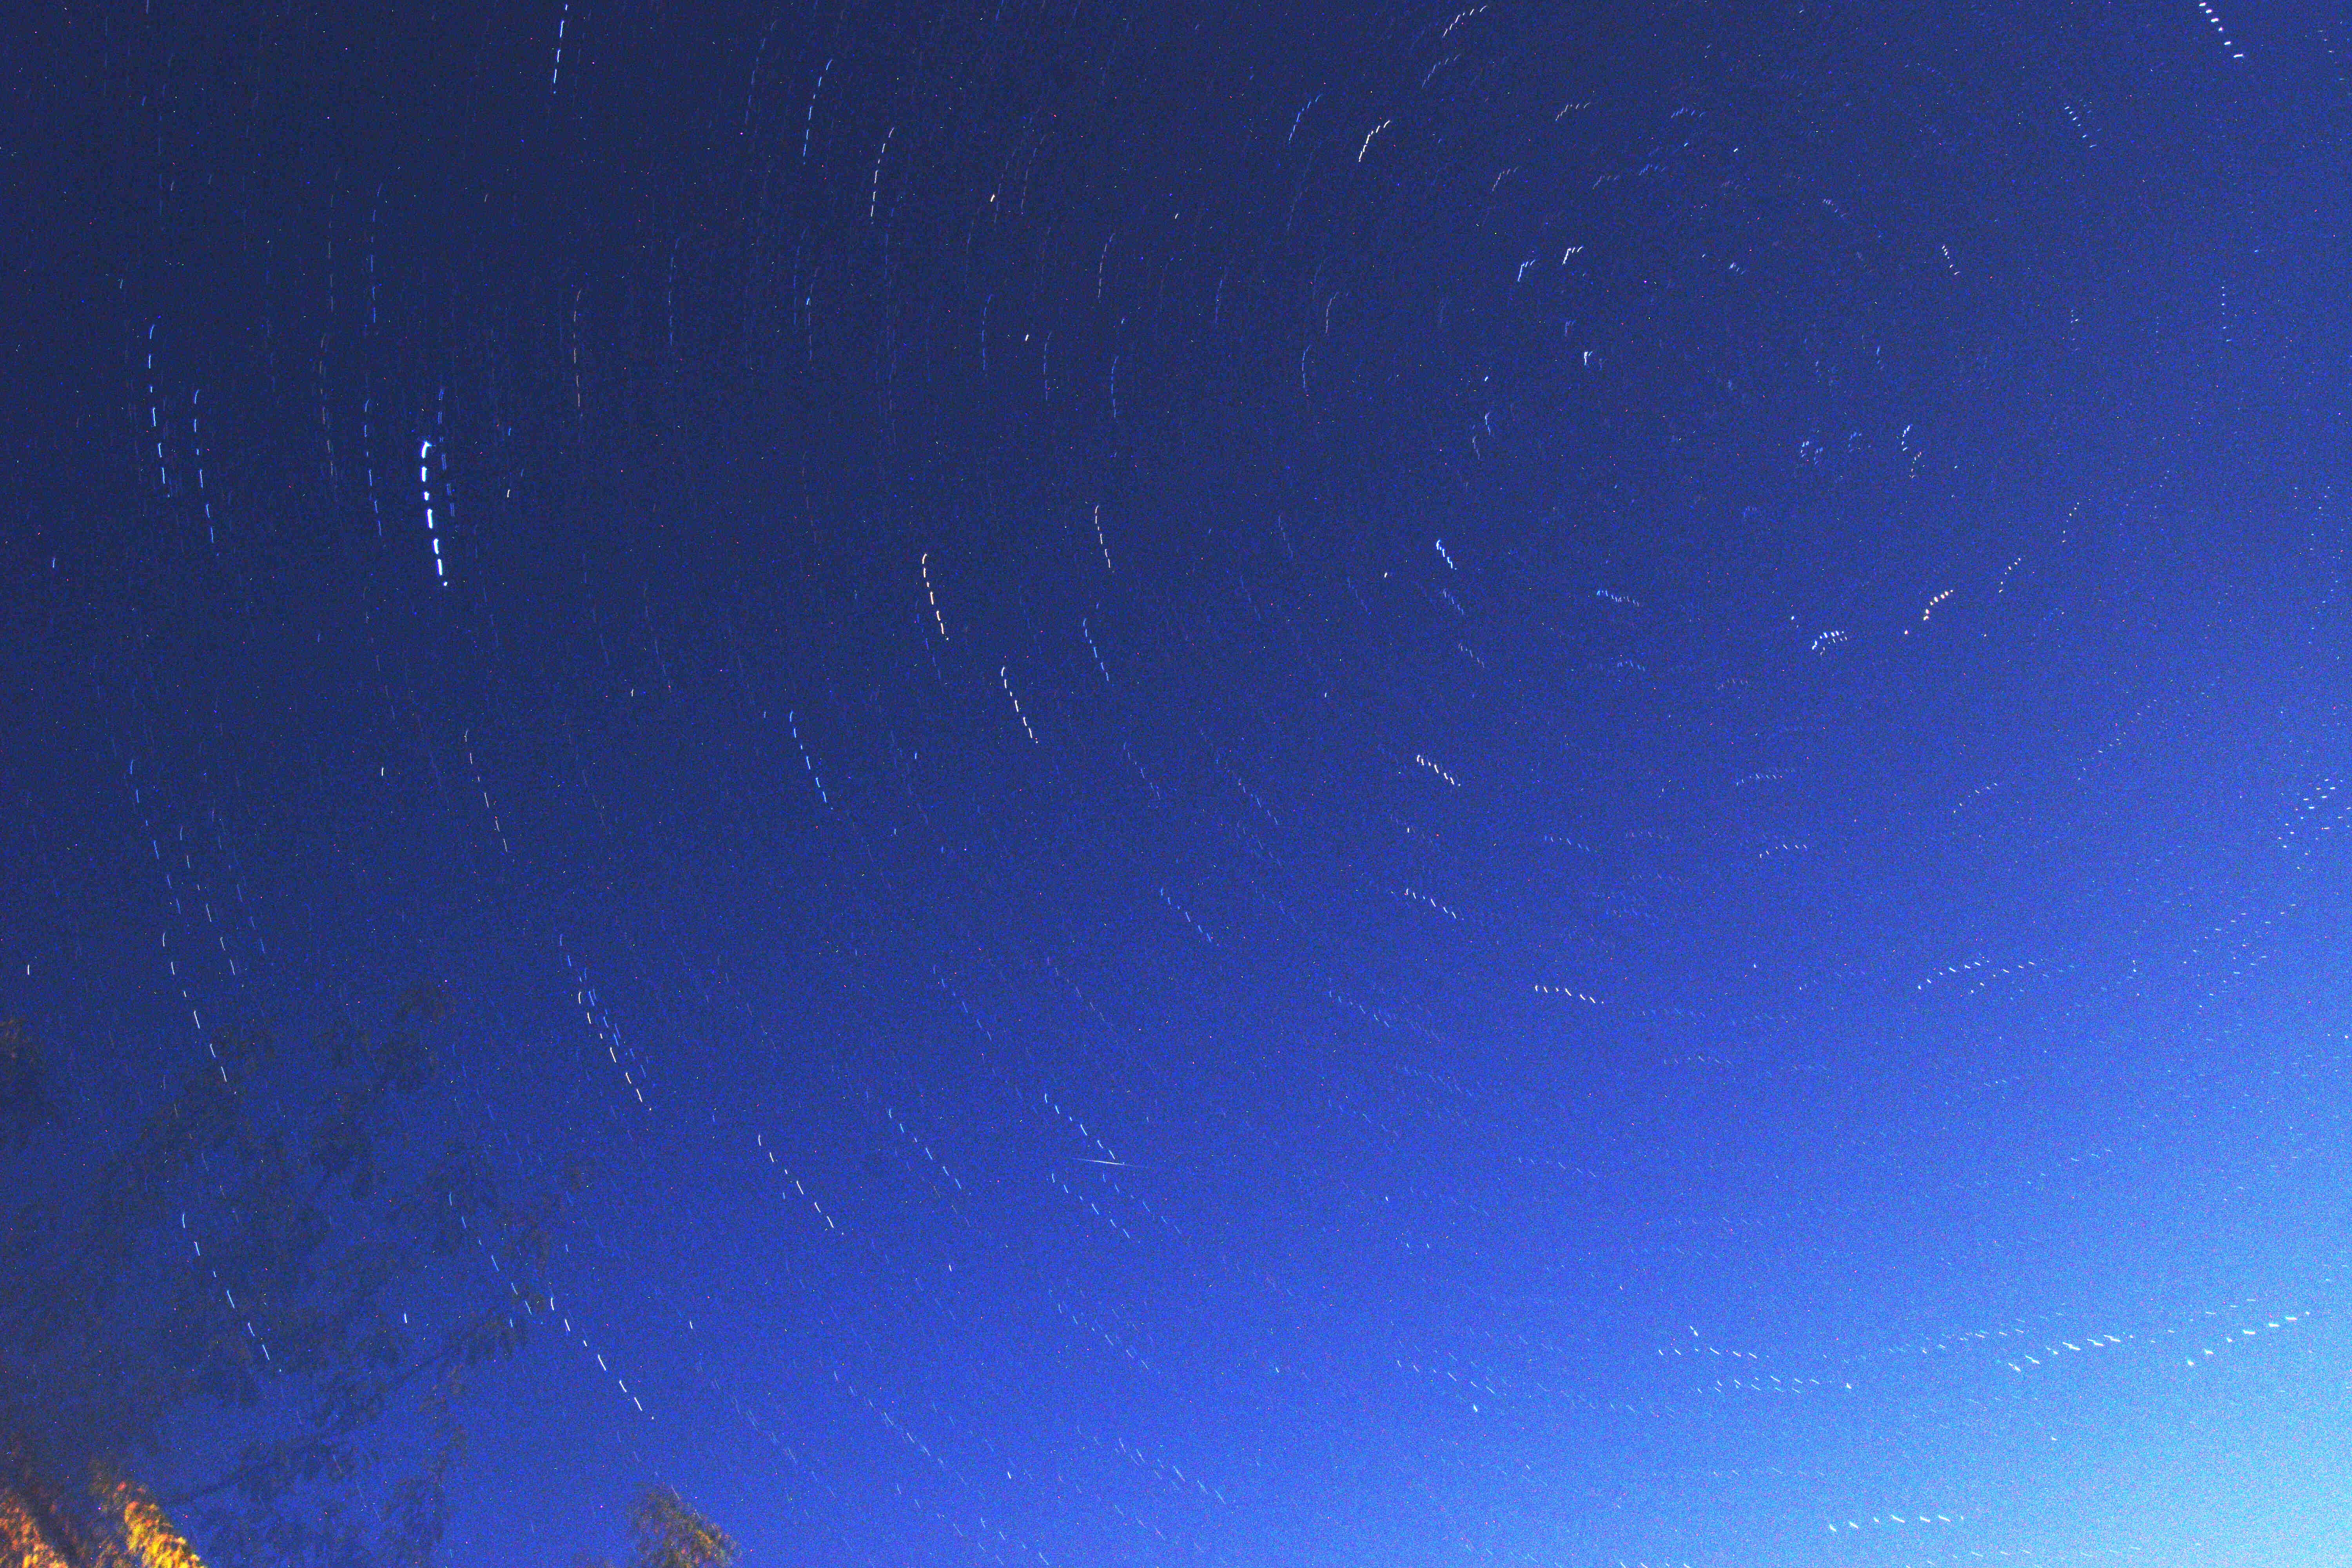
\includegraphics[width=0.8\linewidth]{images/results/DSC_2301}}
	\caption{Some photos taken with the star tracker. The star trail, which should not be present, is visibile.  }
	\label{fig:startrackerresult}
\end{figure}

The pictures where enhanced with Gimp. As can be clearly seen, not only there is a visible star trail, which should not be there, but it is also irregular and scattered. These visual problems derive primarily from misalignment and periodic error \cite{fieldrotation}, due to inaccuracies in the gears.

\section{Conclusion}

There are several design issues, which make the star tracker not functional, as showed in the previous section. The main problems are:

\begin{itemize}
	\item 3d printing: the printer used to make the parts, Creality Ender 3 Pro, is not suitable for the kind of precision required for the gears and other parts. This is particularly obvious from the motor in the \textit{base} part, which originally was intended to rotate the upper parts, but due to the inability to accomplish this it was decided to use it as simple "vibrator" device. This comes from excessive friction between the parts, and probably a not totally correct placement. Other parts where the inaccuracy of the printing is visible is in the middle part, which does not form a regular "u" shape. Finally, the material itself, \textit{pla}, is not really suitable for this project, since it is prone to deterioration and deformation;
	\item General design issues: this design does not allow to comfortably use a system of counterweight placed on top of an arm to set the camera on the \textit{top} plane, since it could hit the top sides of the \textit{middle} part. Although it was not initially considered in order to keep the design the simplest possible, it is not possible to easily integrate one without changing the main design. Commercial systems make use of this solution, because it relieves a lot of effort from the motor that has to move the camera, and also allows for heavier cameras to be used;
	\item gears: the gears take a lot of space and provide little ratio, especially the gears used in the tracking: other gears systems, such as ones involving \textit{worm} gears, allow for greater ratio, thus allowing smoother rotations and less wait time between microsteps, which in turn allows for higher focal lengths;
	\item general (im)precision: the star tracker is not very precise in its alignment operations: the magnetometer is easily interfered with near electromagnetic fields due to its nature, and the tilt plane is continually altered due to the lack of sturdiness of the structure. Furthermore, some parts are not correctly placed: e.g. the \textit{top} plane has a slightly yaw angle, instead of being levelled with the ground, adding additional inaccuracies. This results in a general lack of precision for the alignment of the \textit{top} plane;
	\item lack of power: the power system design fails to provide the right amount of current, e.g. due to the DC-DC converters that low the current output. This results in missteps during the tracking, and in more than one occasion the camera slipped when should have been moved slowly. 
\end{itemize}

All these problems make the tracking inaccurate, and not fully happening. The interrupted smudges in the photos in the previous section are due to lack of tracking during microsteps, and a sudden movement of the gear, because the gears do not provide enough contact due to inaccuracies of their printing, and the motor cannot provide enough torque during all the step duration. 
\\
\\
But in conclusion, while the electro-mechanical problems can be overcome with a redesign and better engineering solutions, the goal to build a cheap auto-alignment system can still be a difficult problem to overcome, since it depends on really imprecise systems, especially the magnetometer. Another way an alignment system could be developed is through making a preliminary photo, identify the stars in the image to compute the current orientation, and then through very precise movements align the star tracker; this however introduces new though challenges on its own.

\newpage
\tableofcontents

\begin{thebibliography}{9}
	\bibitem{shotnoise}
	What's that noise? Part one: Shedding some light on the sources of noise
	
	\url{https://www.dpreview.com/articles/8189925268/what-s-that-noise-shedding-some-light-on-the-sources-of-noise}
	
	\bibitem{microscope}
	The Micro Scope | a Miniture GOTO Telescope.
	
	\url{https://www.instructables.com/The-Micro-Scope-a-Miniture-GOTO-Telescope/}
	
	\bibitem{openastrotracker}
	OpenAstroTech
	
	\url{https://openastrotech.com/}
	
	\bibitem{ogstartracker}
	The OG Star Tracker
	
	\url{https://github.com/OndraGejdos/OG-star-tracker-}
	
	\bibitem{ogstartrackerreddit}
	OG star tracker : Fully 3d printed star tracker that you can make at home is relesing today
	
	\url{https://www.reddit.com/r/functionalprint/comments/10ehxgr/og_star_tracker_fully_3d_printed_star_tracker/}
	
	\bibitem{cosmos}
	Sidereal Day, \textit{COSMOS - The SAO Encyclopedia of Astronomy}
	
	\url{https://astronomy.swin.edu.au/cosmos/s/Sidereal+Day}
	
	\bibitem{nikon}
	Understanding Focal Length
	
	\url{https://www.nikonusa.com/en/learn-and-explore/a/tips-and-techniques/understanding-focal-length.html#}	
	
	\bibitem{cropfactor} What is Crop Factor?
	
	\url{https://photographylife.com/what-is-crop-factor}
	
	\bibitem{500rule} The 500 Rule
	
	\url{bhttps://astrobackyard.com/the-500-rule/}
	
	\bibitem{magndecl} Geomagnetism Frequently Asked Questions 
	
	\url{https://www.ncei.noaa.gov/products/geomagnetism-frequently-asked-questions}
	
	\bibitem{polaralignment} Polar Alignment for Beginners – Step by Step
	
	\url{https://astrobackyard.com/polar-alignment/}
	
	\bibitem{drift} King's polar drift method
	
	\url{https://canburytech.net/DriftAlign/DriftAlign_4.html}
	
	\bibitem{fieldrotation} Diagnosing Trailed Stars
	
	\url{https://www.astropix.com/html/astrophotography/diagnosing_trailed_stars.html}
	
	\bibitem{steppermotors}
	Bipolar Stepper Motors (Part I): Control Modes 
	
	\url{https://www.monolithicpower.com/bipolar-stepper-motors-part-i-control-modes}
	
	\bibitem{microstepping}
	What is microstepping?
	
	\url{https://www.linearmotiontips.com/microstepping-basics/}
	
	\bibitem{torquevoltage}
	Stepper Torque vs Voltage
	
	\url{https://embeddedtronicsblog.wordpress.com/2020/09/23/stepper-torque-vs-voltage/}
	
	\bibitem{i2cadafruit}
	 Software I2C 
	 
	 \url{https://learn.adafruit.com/raspberry-pi-i2c-clock-stretching-fixes/software-i2c}
	 
	\bibitem{mtspecs} MT3608 - High Efficiency 1.2MHz 2A Step Up Converter
	
	 \url{https://www.olimex.com/Products/Breadboarding/BB-PWR-3608/resources/MT3608.pdf}
	
	\bibitem{steppermcurrent}  The Effect of Speed on Stepper Motor Torque Performance 
	
	\url{https://www.portescap.com/en/newsroom/blog/2023/09/the-effect-of-speed-on-stepper-motor-torque-performance}
	 
	\bibitem{mteffspec} Efficiency \& noise of an MT3608 boost module
	
	\url{https://embedblog.eu/?p=712}
	
	\bibitem{powerbenchmark} Power consumption benchmarks
	
	\url{https://www.pidramble.com/wiki/benchmarks/power-consumption}
	
	\bibitem{vectornav} Magnetometer Hard \& Soft Iron Calibration
	
	\url{https://www.vectornav.com/resources/inertial-navigation-primer/specifications--and--error-budgets/specs-hsicalibration}
	
	\bibitem{calibsw} Magnetometer calibration
	
	\url{https://github.com/nliaudat/magnetometer_calibration}
	
	\bibitem{asyncpython} Async IO in Python: A Complete Walkthrough
	
	\url{https://realpython.com/async-io-python/#reader-comments}
	
	\bibitem{wmm2020} World Magnetic Model (WMM), \textit{National Centers for Environmental Information}
	
	\url{https://www.ncei.noaa.gov/products/world-magnetic-model}
	
	\bibitem{gps_nmea} Interface ublox NEO-6M GPS Module with Arduino
	
	\url{https://lastminuteengineers.com/neo6m-gps-arduino-tutorial/}
	
	\bibitem{sparkfun} MPU-6000 and MPU-6050 Register Map and Descriptions Revision 4.0
	
	\url{https://cdn.sparkfun.com/datasheets/Sensors/Accelerometers/RM-MPU-6000A.pdf}
\end{thebibliography}

\end{document}
